% Master-Thesis: Indoor self-localization with Smartphones using iBeacons
% Thomas Bopst (MSI)
% HTWG-Konstanz
%
% Date: 01.10.2014
%

\documentclass[11pt,a4paper]{report}

% Own packages
\usepackage[utf8]{inputenc}
\usepackage[german, english]{babel}
\usepackage{courier}
\usepackage[]{natbib}

\usepackage{listings}
\lstset{numbers=left, numberstyle=\tiny, numbersep=20pt} % Programmcode einfügen
\lstset{basicstyle=\normalsize\ttfamily, breaklines=true} % \footnotesize
\lstset{language=XML}

\usepackage{pgfplots}
\usepackage{subfig}
\usepackage{floatrow}
\usepackage{mathtools}

\selectlanguage{english}

\usepackage[printonlyused]{acronym}
% PDF Eigenschaften
% -----------------
\usepackage
[
	colorlinks = false,
	bookmarks = true,
	pdftitle={Master-Thesis Indoor self-localization with Smartphones using iBeacons},
	pdfauthor={Thomas Bopst},
	pdfsubject={Master-Thesis},
	pdfkeywords={HTWG-Konstanz, Master-Thesis, MSI},
	urlcolor=blue,
	pdfstartview=FitH
]{hyperref}

\usepackage{titlesec}
\titleformat{\chapter}[display]
{\normalfont\huge\bfseries}{\chaptertitlename\ \thechapter}{20pt}{\Huge}
\titlespacing*{\chapter}{0pt}{-40pt}{20pt}

% HTWG-Template
\usepackage{graphicx}
\usepackage{a4wide} % HTWG a4
%\usepackage[english]{babel}

% HTWG-Template
\newcommand{\thema}{Indoor self-localization with Smartphones
 using iBeacons}
\newcommand{\schlagworte}{Indoor Localization, iBeacons, Particle Filter, Monte Carlo Localization}
\newcommand{\zusammenfassung}{Location-based applications are nowadays taken for granted in our life, but until now the available indoor localization systems have not been able to establish themselves. At their \acs{WWDC}~2013 Apple introduced a new technology called iBeacons. This relies on small and cheap \acl{BLE} chips which enables new location awareness features \citep{apple:wwdc_2013_bruins}.

In this thesis I propose a new indoor self-localization solution based on \acl{PF}, respectively \acl{MCL}, by combining \acs{RSS} based distance estimations to deployed beacons, with the user's motion, as determined by the smartphone's built-in sensors. In addition map information, such as free and occupied space, is used.

As a result, this approach solves the global localization problem, and is also able to detect and to recover from failure state. During my experiments, I was able to estimate a user’s stationary location, with a mean error of 2.29~m. Furthermore, I was able to track a user’s path in my test environment.}
\newcommand{\ausgabedatum}{01.11.2014}
\newcommand{\abgabedatum}{01.01.1900}
\newcommand{\autor}{Thomas Bopst}
\newcommand{\autorStrasse}{Albert-Gebhardt-Str. 5}
\newcommand{\autorPLZ}{79761}
\newcommand{\autorOrt}{Waldshut-Tiengen}
\newcommand{\autorGeburtsort}{München}
\newcommand{\autorGeburtsdatum}{31.01.1990 }
\newcommand{\prueferA}{Prof. Dr. Oliver Bittel}
\newcommand{\prueferB}{M.Sc. Michael Blaich}
\newcommand{\firma}{HTWG-Konstanz}
\newcommand{\studiengang}{Master of Science Informatik}


\begin{document}

% select language
\selectlanguage{german}

 % set pagecount style to i,ii,...
\setcounter{page}{1}
\pagenumbering{roman}


% HTWG-Template
% -------------

\begin{titlepage}

\vspace*{-3.5cm}

\begin{center} %flushleft
\hspace*{-1cm} 
\includegraphics[width=15.7cm]{figures/htwg-logo}
\end{center} %flushleft

\vspace{2.5cm}

\begin{center}
	\huge{
		\textbf{\thema} \\[5cm]
	}
	\Large{
		\textbf{\autor}} \\[6.5cm]
	\large{
		\textbf{Konstanz, \abgabedatum} \\[2.3cm]
	}

	\Huge{
		\textbf{{\sf MASTERARBEIT}}
	}
\end{center}

\end{titlepage}

\thispagestyle{empty}
{
\setlength{\parskip}{0.5cm}
        \begin{center}
        \textbf{\huge MASTERARBEIT}

        \textbf{zur Erlangung des akademischen Grades}

        \textbf{\Large Master of Science (M. Sc.)}

        \textbf{an der}

        \textsf{\huge Hochschule Konstanz}\\
        {\small Technik, Wirtschaft und Gestaltung}

        \textsf{\Large Fakultät Informatik} \\
        Studiengang \studiengang
        \end{center}
}
\begin{center}

\vspace*{2cm}

\begin{tabular}{p{3cm}p{12cm}}
Thema: & \textbf{\large \thema} \\[15ex]
Masterkandidat: & \autor, \autorStrasse, \autorPLZ  \autorOrt \\[15ex]
1. Prüfer: & \prueferA \\
2. Prüfer: & \prueferB \\[25ex]
Ausgabedatum: & \ausgabedatum \\
Abgabedatum: & \abgabedatum \\
\end{tabular}
\end{center}


\begin{center}
{\Large \textbf{Zusammenfassung (Abstract)}}
\end{center}

\bigskip

\begin{center}
	\begin{tabular}{p{2.8cm}p{10cm}}
		Thema: & \thema \\
		 & \\
		Masterkandidat: & \autor \\
		 & \\
		Hochschule: & \firma \\
		 & \\
		Betreuer: & \prueferA  \\[.5ex]
		 &  \prueferB \\
		 & \\
		Abgabedatum: & \abgabedatum \\
		 & \\
		Schlagworte: & \schlagworte \\
		 & \\
	\end{tabular}
\end{center}

\bigskip

\noindent
\zusammenfassung

\chapter*{Ehrenwörtliche Erklärung}
\addcontentsline{toc}{chapter}{Ehrenwörtliche Erklärung}

Hiermit erkläre ich
\textit{\autor, geboren am \autorGeburtsdatum in \autorGeburtsort}, dass ich\\

\begin{tabular}{lp{12cm}}
(1) & meine Masterarbeit mit dem Titel \\[1em]
& \textbf{\thema} \\[1em]
& an der \firma\ unter Anleitung von \prueferA\ selbständig und ohne fremde Hilfe angefertigt und keine anderen als die angeführten Hilfen benutzt habe;\\[1em]
(2) & die Übernahme wörtlicher Zitate, von Tabellen, Zeichnungen, Bildern und
Programmen aus der Literatur oder anderen Quellen (Internet) sowie die Verwendung
der Gedanken anderer Autoren an den entsprechenden Stellen innerhalb der Arbeit
gekennzeichnet habe.\\
\end{tabular}

\vspace*{1cm}

\noindent
Ich bin mir bewusst, dass eine falsche Erklärung rechtliche Folgen haben wird.\\

\vspace*{3cm}

\noindent
Konstanz, \abgabedatum \hfill \begin{tabular}{c} \\ \\ \rule{5cm}{1pt} \\ (Unterschrift)\end{tabular}


% change language to english
\selectlanguage{english}

% Abbreviations
\chapter*{Abbreviations}
\addcontentsline{toc}{chapter}{Abbreviations}

\begin{acronym}[BLE]
 \acro{AOA}{Angle of Arrival}	
 \acro{App}{Application}
 \acro{API}{Application Programming Interface}
 \acro{BLE}{Bluetooth Low Energy}
 \acro{BR}{Basic Rate}
 \acro{BT}{Bluetooth}
 \acro{CL}{CoreLocation}
 \acro{CM}{CoreMotion}
 \acro{CPU}{Central Processing Unit}
 \acro{EDR}{Enhanced Data Rate}
 \acro{EKF}{Extended Kalman Filter}
 \acro{GPS}{Global Positioning System}
 \acro{KF}{Kalman Filter}
 \acro{LE}{Low Energy}
 \acro{MAC}{Media Access Control}
 \acro{MCL}{Monte Carlo Localization}
 \acro{MEMS}{Microelectromechanical Systems}
 \acro{NDF}{Normal Distribution Function}
 \acro{OS}{Operating System}
 \acro{PF}{Particle Filter}
 \acro{UI}{User Interface}
 \acro{UUID}{Universal Unique Identifier}
 \acro{LOS}{Line-of-sight}
 \acro{RSS}{Received Signal Strength}
 \acro{RSSI}{Received Signal Strength Indicator}
 \acro{RTOF}{Roundtrip Time of Flight}
 \acro{RX}{Receiver}
 \acro{TDOA}{Time Difference of Arrival}
 \acro{TOA}{Time of Arrival}
 \acro{TX}{Transmitter}
 \acro{WWDC}{Worldwide Developers Conference}
\end{acronym}

\newpage

% Table of contents
\tableofcontents
\newpage
%\listoffigures
%\listoftables

% Content
% -------
\setcounter{page}{1} % set pagecount style to 1, 2, ...
\pagenumbering{arabic}

\chapter{Introduction} \label{chap:intro}

Wouldn't it be great, to being guided on the airport while hurrying from the arrival to the departure gate? Wouldn't it be fantastic, to have the smartphone guiding oneself on a huge trade fair from one interesting fair stand to the next one? Wouldn't it be awesome, to enter a shopping list in oneself's favorite grocery store's app, and then being guided through the store, on the shortest and quickest path?

%\section{Problem}
Location-based applications, have a permanent position in our life. A few years ago, the probably most popular location-based application, \acs{GPS} based navigation systems, drastically improved our navigation skills on street, by replacing the old paper maps. Today, \acs{GPS} based applications are an elementary feature of smartphones. We use them on a daily basis, to determine our position in new cities and on trails, or to track our sports activities. But, all of them works just outdoors, because \acs{GPS} requires \acl{LOS}, for accurate location estimation.

In the area of mobile indoor robotics, indoor self-localization is a well known problem. Robots are equipped with sensors, such as odometers, laser scanners or ultrasonic sensors, to determine their position. Humans are typically not equipped with sensors, but smartphones, our permanent companions, contain lots of them, to perceive our environment.

Actually, approaches for indoor self-localization with smartphones, based on WiFi or Bluetooth, do exist, but until now, they did not manage to get established in our, resp.\ the mainstream's, daily life. From my point of view it is a chicken-and-egg problem. Most people do not know that technically indoor localization is possible and thus, the owners of buildings feel no pressure to provide the necessary infrastructure. On the other side building owner's will not invest on their part, due to the expensive infrastructure. Consequently, people should get to be aware of these possibility, or the infrastructure needs to get cheaper.

Apple addressed both problems at the same time by introducing a new technology, called \emph{iBeacon}, at their yearly \ac{WWDC} in June~2013. iBeacons are small hardware chips equipped with a \ac{BLE} module. Capable smartphones can receive their \acs{BLE} signals to estimate the proximity to a beacon. \citet{apple:ibeacon_site} promotes the technology, on their iBeacon developer website, with the following use-cases: ``From welcoming people as they arrive at a sporting event to providing information about a nearby museum exhibit, iBeacon opens a new world of possibilities for location awareness, and countless opportunities for interactivity between iOS devices and iBeacon hardware.'' Finally, the press made them popular by adding the use-case \emph{indoor navigation}, to solve problems as the above stated ones.

% zu kompliziert, läufte fordern sie nicht genug, jedoch auch zu teuer und komplex für shops und anbieter
% additionally use sensors in smartphone
% location-based applications broad appeal (navigation, robotics, gaming, asset tracking, ...)
% no GPS, loss of signal, or very bad accuracy
\section{Requirements}
From our point of view an indoor self-localization system should satisfy the following requirements. The system should be usable with common devices. Therefore, it needs to be cross-platform. Additionally, the system should be of low cost for both, the building owner and the user. Consequently, the system's infrastructure should be as simple as possible. The system should also be easy-to-deploy, and cause less maintenance costs. Besides that, the user's device and application's algorithm should be as independent as possible from the remaining infrastructure. Thus, localization should take place on the user's device.

\section{Idea}
The idea is to design, implement and evaluate an indoor self-localization systems with Smartphones using iBeacons, which satisfies the before mentioned requirements.

Therefore, common smartphones equipped with a \acs{BLE} module can be used. Our solution is based on \ac{MCL}. The smartphone's build-in sensors are being used to measure the user's motion. The algorithm requires also a map of its environment. Additionally, the proximity to known beacons is being integrated into the position estimation.

The designed solution can run on every platform. iBeacons are relatively cheap and require no additional infrastructure, such as a power supply or network connection. They can be powered with a small battery or a coin cell over months. Also, the deployment is very simple. The beacons just need to be spread over the area, where the localization should take place. Additionally an initial calibration step needs to be performed. If the beacons environment does not change, no maintenance is necessary. The user's device is completely independent. The whole position estimation takes place on the user's device. No connection between smartphone and the remaining infrastructure is being established.


%Use approach from robotics.
%
%Ein Grund Q/A [Apple intro], says it is not possible to show precise location.
%
%UseCase:
%\begin{itemize}
%  \item (assets management, staff tracking,) indoor tourist guiding in museums, train stations, airport, shopping complex \citep{wang:bt_pos}, mobile guides, indoor navigation
%  \item example ADAMANT (airport travelers guide) \citep{wang:bt_pos}
%  \item In robotic indoor localization alter hut
%\end{itemize}
%
%Requirements:
%\begin{itemize}
%\item low cost
%\item public available device
%\item cross platform
%\item every thing on device \citep{wang:bt_pos}
%\item easy-to-deploy \citep{wang:bt_pos}
%\end{itemize}
%
%Map with beacon positions

\section{Structure}
The document is split up into seven chapters. First, we give an overview about localization in general, localization algorithms, and related work, in chapter~\ref{chap:fundamentals}. Then, chapter~\ref{chap:ibeacons} gives a detailed insight into iBeacon technology, including \acs{BLE}, configuration parameters, the \acs{API} provided by Apples iOS 8 operating system, and the signal's quality. Afterwards, we are taking a close look, in chapter~\ref{chap:sensors}, on the smartphones build-in sensors, the provided \acsp{API} and the provided data, which we are going to evaluate at the chapter's end. After founding the basis, we present our algorithms implementation in chapter~\ref{chap:pf}, which is a proof of concept, which is being evaluated in chapter~\ref{chap:evaluation}. Finally, we conclude our research in chapter~\ref{chap:conclusion}, including ideas, how the project could be developed further.



\chapter{Fundamentals}\label{chap:fundamentals}

In this chapter, first the basics of localization are introduced. Afterwards, an overview of different localization approaches being used in related work, is given. At the end, I focus on the \acl{PF} and the \acl{MCL} algorithm, which I have chosen for my implementation. The detailed reasons for choosing \ac{MCL} for this project are pointed out in Section~\ref{sec:algo_decision}.

\section{Fundamental Aspects of Localization}\label{sec:fund_loc}

Localization, i.e.\ positioning, is the process of estimating the position of an object in its environment. Usually the object's environment is being defined by using a coordinate system. One of the most popular coordinate systems is the \emph{World Geodetic System 1984 (WGS84)}, which describes a position on earth, by longitude and latitude. Sometimes, it is sufficient to use a local coordinate system; for instance, a two or three dimensional cartesian coordinate system. Indoor localization is one example, where it is sufficient to use a local coordinate system, because the object's position is limited to a defined area, e.g.\ within a building.

\subsection{Location Types}
There are four types of locations. A \emph{physical location} is described by coordinates on a map. \emph{Symbolic locations} such as ``in the living room'' or ``on the small table in the kitchen'', are often used by humans. If all objects are sharing a frame of reference, like chess pieces on a chess board, the type of location is called an \emph{absolute location}. When an object has its own reference frame, as for instance when saying ``I am two meters away from the door'', which often includes a proximity value, it is called a \emph{relative location} \citep{IEEE:survey_wireless_indoor_pos}.

Typically indoor localization is based on absolute locations, because all objects, such as landmarks, obstacles (i.e.\ occupied space), and corridors (i.e.\ free space) share the same frame of reference, i.e.\ the building's map. It is also possible to use physical locations for indoor positioning by either transforming the objects' absolute positions into physical positions or by knowing them. In the following a location is usually a absolute location.

\subsection{System Topology}
Usually, a pure wireless localization system consists of at least one transmitter that emits some sort of signal, and one or more receivers, i.e.\ measuring units. The system's topology can be \emph{remote positioning}, which means that the transmitter's position is being estimated by using the measurements from multiple measuring units, that are deployed at fixed locations. The position estimation takes place in a component separate from the transmitter. This component uses the measurements as input. If the measurement unit is mobile and capable to estimate its own position by collecting the signals from fixed transmitters, the system's topology is called \emph{self-positioning}. \emph{Indirect remote positioning} is basically the same as self-positioning, but the collected measurements are sent via some data connection to an external service, which performs the position estimation. If the system's topology is basically remote positioning, but the measurements are transferred via a wireless data link to the mobile side, the topology is called \emph{indirect self-positioning} \citep{IEEE:survey_wireless_indoor_pos}.

Besides a pure wireless localization systems, which just uses wireless signals for the positioning, other systems, often used in the area of mobile robotics, do exist. Robots are often equipped with sensors, such as laser scanners or ultrasonic sensors, to measure distances to obstacles. Wheel- and chain-based robots are usually also equipped with odometers, others have accelerometers and rotation rate sensors to estimate the traveled distance. The used localization algorithms are able to combine different sensors to provide a more accurate estimation \citep{thrun:prob_robo}. Mobile robots, especially if they operate autonomously, are usually self-positioning, or indirect remote positioning systems, which often depends on their system's hardware capabilities. Remote positioning as well as indirect self-positioning systems are rarely the case in the field of mobile robots.

The proposed solution is a self-positioning system. It measures the distances to known beacons, but it not only relies on the measured wireless signals, it uses also the user's motion, like a robot. Thus, the user's smartphone is the mobile measuring unit, which additionally does the whole position estimation.

\subsection{Uncertainty}
In order to derive an accurate position, localization systems need to be able to accommodate uncertainty. According to \citet{thrun:prob_robo}, uncertainty in robotic systems has several reasons.

One of these reasons is the \emph{environment}. If a robot works together with humans, the environment is very dynamic and unpredictable, because the robot does not know for; instance, where and when a human moves to.
Of course, robots are equipped with \emph{sensors} to recognize obstacles like humans, but sensors may also cause uncertainty. On one hand, they have limitations, e.g.\ a camera has a specific resolution, and on the other hand, noise may unpredictably influences their measurements. 
Typically, robots have \emph{actuators}; for instance, motors to move them within their environment. Actuators have precision limitations. Additionally, their successive physical components; for instance, a robot's wheels on different surfaces, may cause unpredictable effects.
To allow robots to operate in a physical environment, models of it are being used. \emph{Models} are abstractions, which approximate a certain object or behavior. Thus, information is being lost, and additionally every model contains some inaccuracy. Robotic systems work in real-time environments. Due to computational reasons, their \emph{algorithms} cannot really operate in real-time. In reality, a physical property changes continuously, but a robot's measurements can only be processed in certain time steps, which causes inaccuracy. 

All mentioned factors together might cause large uncertainty. Thus, the system needs to be able to accommodate or somehow compensate for it. This is the reason, why the algorithm, introduced in Chapter~\ref{chap:pf}, not only relies on the distance measurements to the beacons. Due to the uncertaintys' high importance, the used sensors' uncertainty is discussed at the end of Chapter~\ref{chap:ibeacons} and \ref{chap:sensors}.

\subsection{Localization Problems}
Localization is not always the same. There are different localization problems depending on the environment and the use-case of the application. According to \citet{thrun:prob_robo} the following problems exist:
\begin{itemize}
\item \textbf{Local vs.\ Global Localization:} If the initial position is known when the localization starts, a so-called position tracking only is necessary, to know future positions. This is called \emph{local localization}. In the case where the initial position is unknown, and this position can by anywhere on the map, this is called \emph{global localization}. These types of algorithms are more difficult than position tracking. Global localization solves also the \emph{kidnapping} problem, which means that e.g.\ a robot is being placed on a different position during the position estimation. Of course, that is not very typically, but by solving this problem the algorithm is also able to recover if it is stuck in a state where it never will be able to approximate the true position.

\item\textbf{Static vs.\ Dynamic Environments:} In a \emph{static environment} the localizing object, e.g.\ a robot, is the only object that changes its position over time. All obstacles and other objects maintain their fixed position. In a \emph{dynamic environment} other objects besides the localizing object can change their position. Typical objects in a dynamic environment are humans, furnitures, like chairs or doors that sometimes are being moved, closed or opened.

\item\textbf{Passive vs.\ Active Approaches:} If the localization algorithm is able to control the localizing object's motion, this is called an \emph{active approach}. Through the ability to influence a motion, the algorithm can induce movement of the of the object, e.g.\ the robot, if the localization is stuck and needs more information; for example, from another point within a room, to decide what its position is. \emph{Passive} algorithms just observe the motion, but cannot influence it. Usually, active approaches are built upon passive ones.

\item\textbf{Single-Robot vs.\ Multi-Robot localization:} \emph{Single-Robot} localization means, that the robot only needs to localize itself. \emph{Multi-Robot} localization requires of course multiple robots in the same area. It builds upon single-robot localization; thus, each robot can estimate its own position. New opportunities arise if the robots can recognize, each other and are able to communicate, to exchange their estimated positions.
\end{itemize}

\noindent The solution presented in this thesis, solves the global localization and kidnapping problem in a dynamic environment; whereas, the in Chapter~\ref{chap:evaluation} presented results where measured in a static environment. The algorithms implementation is a passive approach. Furthermore, the solution only solves the Single-``Robot'' localization problem, but Chapter~\ref{chap:conclusion} presents an idea how Multi-``Robot'' localization could be used to improve the presented solution.

\subsection{Performance Metrics}
To be able to compare different localization systems and algorithms, the following criteria, recommended by \citet{IEEE:survey_wireless_indoor_pos}, is introduced. Often the system's accuracy is the only metric being used, but also from my opinion as well, the system's accuracy is not sufficient enough for evaluation purposes. In addition to the metrics recommended by \citet{IEEE:survey_wireless_indoor_pos}, the system's usability is another important criteria, in my opinion.
\begin{itemize}
	\item \textbf{Accuracy} is the error of the estimated position. It is the Euclidean distance between the estimated and the real position.
	\item \textbf{Precision} takes the consistency into account. \citet{IEEE:survey_wireless_indoor_pos} defines it as the result of ``the cumulative probability function[s] (CDF) of the distance error'', for instance 90\% location precision within 2m ($CDF(2m) = 0.9$).
	\item \textbf{Complexity} depends on several factors, such as the required hardware, the software complexity, the algorithms complexity, the necessary infrastructure, etc. However, \citet{IEEE:survey_wireless_indoor_pos} focus on software, i.e.\ computing complexity only.
	\item \textbf{Robustness} expresses the ability of a system to deal with wrong sensor data, unexpected values, or even no sensor data within a certain time interval.
	\item \textbf{Scalability} describes the possibility of a system to be extended or reduced in space, or a change of the density of the transmitters or measurement units.
	\item \textbf{Cost} depends on several factors. The financial costs are a very important factor. This depends on the hardware, implementation and installation costs. The energy consumption, which in the end also reflects in financial cost, is also an important factor. The factor time is also not negligible. The amount of time it takes to deploy and maintain such a system can be enormous.
	\item \textbf{Usability} depends mainly on the system's user friendliness, i.e.\ is it difficult for the user to use the system, is the system self-explaining, etc. If a system's usability is very bad its usually not being accepted by the users.
\end{itemize}

\noindent In Chapter~\ref{chap:evaluation}, the presented solution is evaluated against these criterias, with focus on the system's accuracy and precision.


\section{Particle Filter Algorithm and Related Work}\label{sec:fund_pf}
The solution proposed in in this thesis builds upon \acf{MCL}, which is based on \acf{PF}. This section introduces first the \ac{PF}'s basics and afterwards the fundamentals of \ac{MCL}. Finally, it gives an overview of related work, based on \ac{PF} and \ac{MCL}.

\subsection{Introduction to \acl{PF}}
The \ac{PF} is a non-parametric filter, i.e.\ it does not have fixed parameters which describe its distribution's functional form. By contrast \acf{KF} is a parametric filter, which parameters describe its functional form, i.e.\ a Gaussian distribution. \ac{PF} approximates the functional form by a finite number of values, often referred to as \emph{particles} or \emph{samples}. The approximation's quality depends on the particle set's size. Figure~\ref{fig:pf_approx} illustrates the approximation of a posterior distribution by samples. It also shows, that particle filter is well-suited for multi-modal beliefs \citep{thrun:prob_robo}.

\begin{figure}
	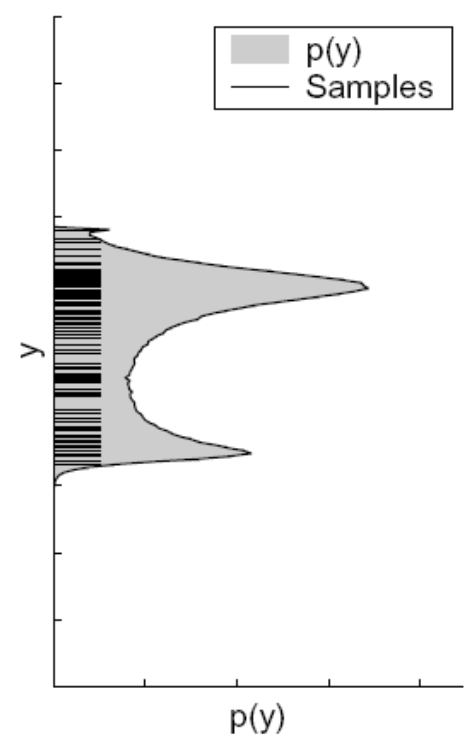
\includegraphics[height=0.45\textwidth]{figures/pf_approx}
	\caption{Approximation of a random variable Y, i.e.\ a posterior distribution by samples \citep[p.97]{thrun:prob_robo}.}
	\label{fig:pf_approx}
\end{figure} 

\begin{lstlisting}[
  float,
  floatplacement=H,
  mathescape,
  captionpos=b,
  caption=Algorithm for \acl{PF} based on \citet{thrun:prob_robo},
  label=lst:pf]
ParticleFilter($\chi_{t-1}$, $u_t$, $z_t$) {

  $\bar{\chi}_t = \emptyset$
  for $m = 1$ to $M$ {
    sample $x^{[m]}_t \sim p(x_t|u_t, x^{[m]}_{t-1})$
    $w^{[m]}_t = p(z_t|x^{[m]}_t)$
    add $\langle x^{[m]}_t, w^{[m]}_t \rangle$ to $\bar{\chi}_t$
  }


  \\ resampling
  $\chi_t = \emptyset$
  while size of $\chi_t$ less $M$ {
    draw $i$ with probability $\propto w^{[m]}_t$
    add $x^{[i]}_t$ to $\chi_t$
  }

  return $\chi_t$
}
\end{lstlisting}
 % label= lst:pf

According to \citet{thrun:prob_robo}, the idea is the posterior's $bel(x_t)$ representation by a random set of samples, drawn from the posterior. Each sample (i.e.\ particle) $x$ at time $t$ is a hypothetical state in state space, i.e.\ in real world. The particle set $\chi_t = \left\{ x^{[1]}_t, x^{[2]}_t, \ldots, x^{[M]}_t \right\}$ is the distribution's approximation, containing $M$ particles. The \ac{PF}'s algorithm, depicted in Listing~\ref{lst:pf}, transforms the $bel(x_{t-1})$, represented by the particle set $\chi_{t-1}$, by integrating the latest control $u_t$ and measurement $z_t$ into the current $bel(x_t)$. Thus, the algorithm creates first an empty, temporary particle set $\bar{\chi}_t$. Then, the states from $\chi_{t-1}$ are being updated by integrating the current control $u_t$. Formally, this is done by sampling the new state $x_t$ from the \emph{state transition probability} $p(x_t|u_t, x^{[m]}_{t-1})$ (Listing~\ref{lst:pf}, Line 5). Afterwards, an \emph{importance factor} $w^{[m]}_t$ for the new sample $x^{[m]}_t$ is being calculated (Listing~\ref{lst:pf}, Line 6). It is defined as $p(z_t|x^{[m]}_t)$, which is the probability for the measurement $z_t$ given the new state hypothesis, representing a value in real world. The new state hypothesis and its importance factor are stored together, as tuple, in the temporary set $\bar{\chi}_t$ (Listing~\ref{lst:pf}, Line 7). The weighted set approximates the $bel(x_t)$.

Then, the resampling, i.e.\ importance sampling, transforms the weighted set, based on their weights into a new set, which represents the new distribution. Therefor, $M$ particles are drawn according their weight and inserted into the new set $\chi_t$ (Listing~\ref{lst:pf}, Line 14, 15). During this step some particles are duplicated, usually the ones with high weight, and others, the ones with low weight, are lost. \citet{thrun:prob_robo} compares it with the Darwinian idea of \emph{survival of the fittest}. According to them, ``it refocuses the particle set to regions in state space with high posterior probability''.
 
Instead of the drawing, it is also possible to have a weighted set $\chi_t$. In every recursion, the weights of the existing particles are multiplied with their new weight. The method's disadvantage is, that a larger particle set is being required to reach the same approximation quality, because the particles keep their position in state space for ever, i.e.\ the particle cloud does not move. For this method the particle weight $w^{[m]}_t$ of each particle needs to be initialized with 1.
 
\ac{PF} can be adaptive; for instance, based on the available processing power. The particle set is then being increased or decreased to adapt to the available processing power \citep{thrun:prob_robo}.


\subsection{Monte Carlo Localization}\label{sec:fund_mcl}
\ac{MCL} is a popular localization algorithm often used in the indoor mobile robotics field. The algorithm can deal with a broad range of the before discussed localization problems, especially with the local and global localization problem.

\begin{lstlisting}[
  float,
  floatplacement=H,
  mathescape,
  captionpos=b,
  caption=Basic \acl{MCL} algorithm based on \citet{thrun:prob_robo},
  label=lst:mcl]
mcl($\chi_{t-1}$, $u_t$, $z_t$, map) {

  $\bar{\chi}_t = \emptyset$
  for $m = 1$ to $M$ {
    $x^{[m]}_t$ = sample_motion_model($u_t$, $x^{[m]}_{t-1}$)
    $w^{[m]}_t$ = measurement_model($z_t$,$x^{[m]}_t$, map)
    add $\langle x^{[m]}_t, w^{[m]}_t \rangle$ to $\bar{\chi}_t$
  }


  \\ resampling
  $\chi_t = \emptyset$
  while size of $\chi_t$ less $M$ {
    draw $i$ with probability $\propto w^{[m]}_t$
    add $x^{[i]}_t$ to $\chi_t$
  }

  return $\chi_t$
}
\end{lstlisting}


The basic algorithm, shown in Listing~\ref{lst:mcl}, is very similar to the \ac{PF}, presented in Listing~\ref{lst:pf}. The sampling from the \emph{state transition probability} is substituted by a method called \texttt{sample\_motion\_model}, which samples the new hypothesis by integrating the control $u_t$ with respect to the robot's motion and its uncertainties during the execution (Listing~\ref{lst:mcl}, Line 5). Furthermore, the \emph{importance factor} calculation is substituted by the \texttt{measurement\_model} function, which depends on the used sensor (Listing~\ref{lst:mcl}, Line 6). It uses the sensor measurements and their uncertainty to calculate the particles' importance factors. It additionally takes the environment's map into account. Usually, the map is being used to calculate the importance factor based on the measurement $z_t$; for instance, the distance to a landmark, where the landmark's position is stored in the map. But a map can also be used to detect particles at impossible positions, and thus to reduce their importance factor. A very detailed description about \acl{MCL} and variations of the algorithm is provided by \citet{thrun:prob_robo}.

\begin{figure}[width=0.9\textwidth, height=0.4\textheight]
	\subfloat[]{
  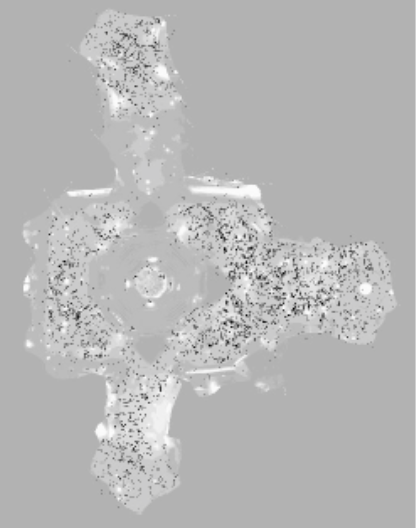
\includegraphics[width=0.3\textwidth]{figures/mcl_1}
}
\subfloat[]{
  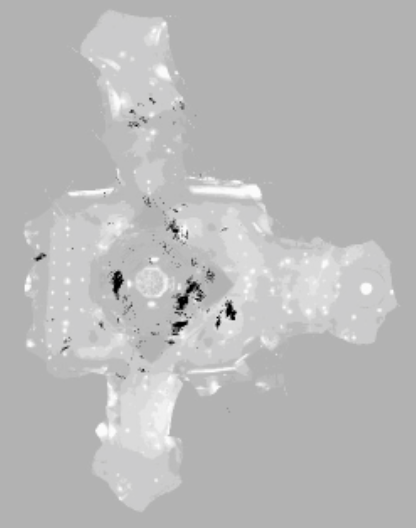
\includegraphics[width=0.3\textwidth]{figures/mcl_2}
}
\subfloat[]{
  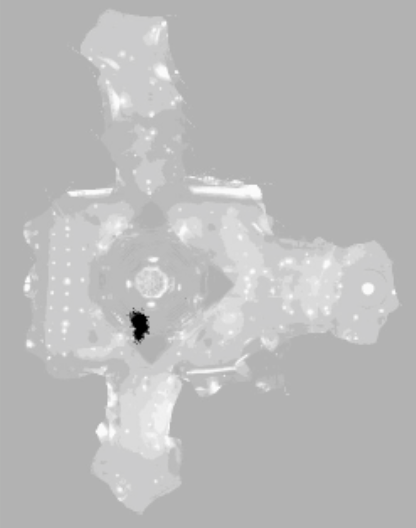
\includegraphics[width=0.3\textwidth]{figures/mcl_3}
}

	\caption{A visual example of the \acl{MCL} algorithm. It shows a building's map and the particle distribution over time \citep{thrun:prob_robo}.}
	\label{fig:mcl}
\end{figure}

A visual example of, how a robot's global localization using \ac{MCL} works, is shown in Figure~\ref{fig:mcl}. The three images show the particles, i.e.\ the posterior $bel(x_k)$, over time. At the beginning uniform random particles are spread over the whole state space, because the robot actually does not know where it is, and thus could be positioned anywhere. After moving and gathering sensor data, the particles concentrate in certain regions with higher probability for the true position. Thus, the posterior changes. In the end, the particles are concentrated on one spot; hence, the confidence of being at this position is very high \citep{thrun:prob_robo}.


\subsection{Related Work}

\citet{Siddiqui:tracking} proposes a localization system that uses \ac{PF} and \ac{RSS}-based trilateration of WiFi signals (explained in Section~\ref{sec:fund_trilateration}), to track a mobile unit. The approach relies solely on sensing \ac{RSS} values, no other sensors are used. First, they collect the \ac{RSS} values in their environment. They are stored together with their location in a lookup table. For their MATLAB simulation they generate a random path with 100~points using the before collected values. The path is tracked during the simulation, just based on the \ac{RSS} values. Their simulation simulates a notebook equipped with WiFi, which is tracked. Thus, their \ac{PF}'s implementation does not sample a new state by integrating the control $u_t$ as shown in Listing~\ref{lst:pf} (line~5). They use two different weighting functions during their experiment, firstly, a \emph{Gaussian weighting function}, based on the Euclidian distance, and secondly, a \emph{Triangular weighting function} (line 6). According to \citet{Siddiqui:tracking}, their solution achieves an accurate localization of $\approx$~3m as a result of their simulation. During the simulation they assume a static environment with sparse activity and a smooth and continuous motion. They also assume that no large variations in the signals' strength occur over short distances. In addition, they remove the first and last 10\% of the recorded measurements, i.e.\ when the person placed the measuring unit and picked it up again, to have their values being independent of a human in proximity. Additionally, they neglect outlliers.

\citet{straub:pf} implemented an indoor pedestrian localization and tracking system based on \ac{PF}, which uses a system called \emph{PiNav}, developed at the institute where Straub wrote his thesis. It extracts the person's motion in form of step frequency, step size, and heading. The person needs to be equipped with the hip-mounted PiNav-System, which includes an accelerometer, gyroscope and a compass. Additionally, \citet{straub:pf} uses an accessibility map, which is based on a Neural Network, to learn which space on the map is accessible by pedestrians. By fusing the pedestrian's motion and the accessibility map in a \ac{PF}, his solution achieves an average accuracy of 1.1m \citep{straub:pf}.

\citet{wang:wlan} propose a \ac{RSS}-based WiFi positioning system using \ac{PF} to fuse the location estimated via WiFi with additional map and accelerometer data. Their system uses the in Section~\ref{sec:fund_sceneanalysis} mentioned scene analysis approach, especially the k-Nearest Neighbors algorithm for the positioning. During the offline stage they collect fingerprints of the WiFi signal in one meter distance to the access points. During the localization, i.e.\ the online stage, the algorithm compares the fingerprints of the collected WiFi signals with the stored ones from the offline stage and returns a location estimation. According to \citet{wang:wlan}, the 3-axis accelerometer's values can be used in theory, to estimate the traveled distance by integrating the values. But, due to the low signal and the sensors' noise it does not work in praxis. Thus, they use a zero-crossing approach to detect steps and estimate their size. The approach detects a step if the vertical acceleration crosses the zero-line. Additionally, their solution uses the environment's map to sort out impossible particles, like particles crossing a wall.
Their simulation results show, that by using map and accelerometer in addition to kNN, their location error improves by 40\%. Their solution is also 30\% better than the \ac{KF}'s result. During their real world tests, they achieved a mean error of 4.3m with a standard deviation of 2.8m \citep{wang:wlan}.

\citet{siddiqi:experiments_mcl_wifi} uses \ac{MCL} to globally localize a \emph{Pioneer 2DX} robot in an indoor environment using the robots odometers and the measured \ac{RSS} of WiFi signals. The algorithm's action model, i.e.\ motion model, is based on the data measured by the odometers. They deliver data for short distances with a very good accuracy. The motion is divided into translations and rotations. Their action model samples the motion with different uncertainties for translation and rotation. The observation model, i.e.\ measurement model, uses a signal strength map, which is divided into a grid with squared fields with a size of 0.5m. Before localization can take place, the \ac{RSS} of each WiFi access point for each grid cell needs to be measured to store \ac{RSS} mean and standard deviation for each cell. Due to the fact, that \citet{siddiqi:experiments_mcl_wifi} assume that the signal attenuation does not change on short distances, they just measured it for a few cells and assumed the same value for the neighbor cells. During the localization, the actual \ac{RSS} values are compared with the collected values for the importance factor. Additionally, their observation model sorts out particles, by using the map constraints, but without taking the robot's orientation into account. According to \citet{siddiqi:experiments_mcl_wifi}, just using the map constraints without the \ac{RSS} comparison, already enables very good localization results.
During their tests they found out, that by increasing the amount of access points, the location error decreases \citep{siddiqi:experiments_mcl_wifi}. They mention, that their approach should also work for localization of humans instead of robots. But they also note, that a robot's motion model is simpler than the one of a human. According to \citet{siddiqi:experiments_mcl_wifi}, they achieved during most test cases an accurate localization with an error of $\approx$~2m.


\section{Further Localization Algorithms and Related Work}
This section focuses on further localization algorithms, which are suitable for indoor self-localization using smartphones. Some algorithms are discussed in more detail than others, depending on their closeness to the solution presented in this thesis. After introducing the algorithm itself, an overview of related work, based on that algorithm, is given.

\subsection{Triangulation}\label{sec:fund_trilateration}
Triangulation is a well-studied localization method which relies on triangle's geometric properties \citep{IEEE:survey_wireless_indoor_pos, wang:bt_pos}. Triangulation is the hypernym of the two characteristics \emph{lateration} and \emph{angulation}.

\begin{figure}[width=0.9\textwidth, height=0.4\textheight]
	\subfloat[Lateration]{
  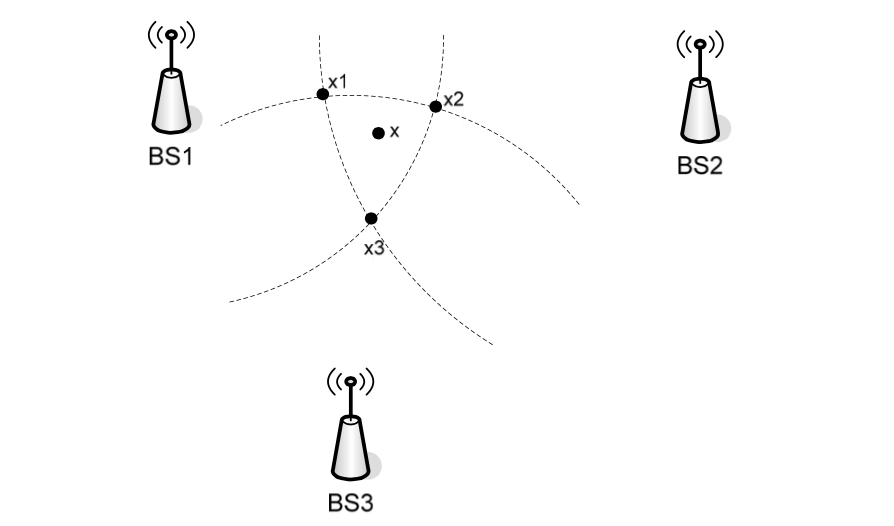
\includegraphics[width=0.45\textwidth]{figures/lateration}
  \label{fig:lateration}
}
\subfloat[Angulation]{
  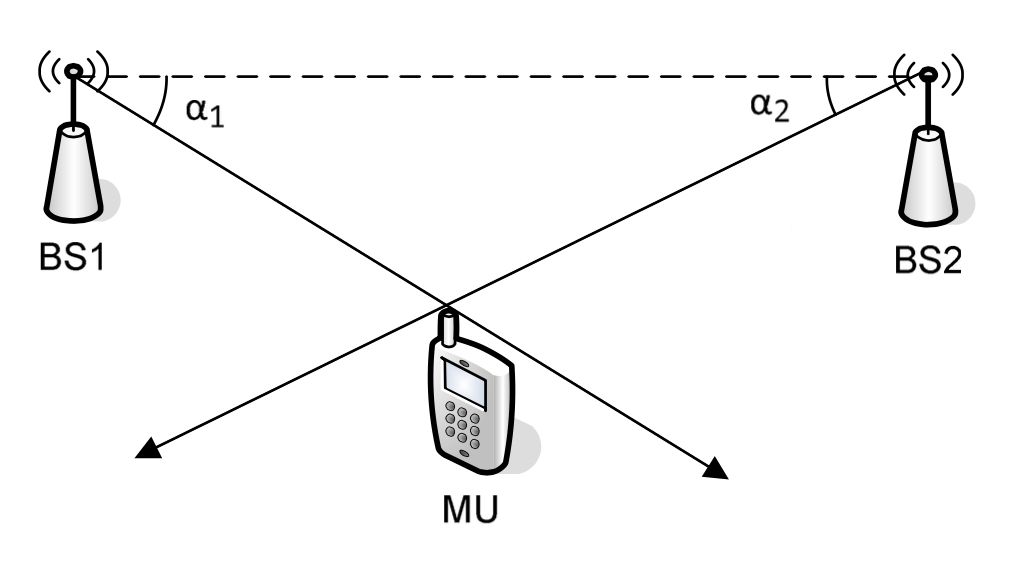
\includegraphics[width=0.45\textwidth]{figures/angulation}
  \label{fig:angulation}
}

	\caption {Principle of the position estimation of a mobile measuring unit using triangulation methods. The wireless signals are transmitted by fixed base stations \citep{wang:bt_pos}.}
	\label{fig:triangulation}
\end{figure}

\subsubsection*{Lateration}
Lateration estimates the location based on the distances from the measuring unit to the transmitters. To precisely estimate a position, three base stations are required. The measuring unit measures the distance to each base station and puts a circle with the radius of the measured distance around the base station. The circles's common intersection point, is the exact position of the mobile unit. In 2D space at least three signals must be received, in 3D, four signals are required. According to \citet{wang:bt_pos}, one common intersection point exists only in theory. In practice, errors, due to obstacles and imperfect propagation models, influence the distances. Thus, no common intersection point exists. Figure~\ref{fig:lateration} depicts this case. Nevertheless, it is possible to estimate the mobile units position by using methods such as least-square, three-boarder, or the centroid-method \citep{wang:bt_pos, IEEE:survey_wireless_indoor_pos}.  

The distance for lateration can be estimated by different methods. According to \citet{IEEE:survey_wireless_indoor_pos}, the distance between the measuring unit and the transmitter is directly proportional to the signal's propagation time.
\emph{\ac{TOA}} uses this fact to estimate the distance by measuring the signal's travel time. Consequently, the transmitted signal contains the timestamp of its transmission. Thus, the clocks of all transmitters and measuring units, that are part of the system, need to be precisely synchronized, in order to perform a correct estimation, which is not a trivial problem. For example a timing difference of 1.0~$\mu s$ in a wireless localization system, such as Wifi or \ac{BT}, causes an error of $\approx$~300m, according to \citet{kotanen:exp_local_pos_bt}.

To overcome this disadvantage, a similar method called \emph{\ac{RTOF}} can be used. This method requires all components to be able to receive and transmit signals. The transmitter sends a signal, it is being received and immediately being returned, by the mobile unit. Thus, the transmitter sets the timestamp and compares it with its current timestamp, when the signal arrives. A relative time synchronization is sufficient enough. But \ac{RTOF} has another problem. The signal is being delayed by the processing time, which the unit requires to receive and to send it back to the original source.

The \emph{\ac{TDOA}} method calculates the distance from the different arrival times at the measuring units. Here, the measuring units need to be connected with each other to exchange the timestamps of the signals' arrival and to precisely synchronize their timestamps. The clocks' differences should not exceed tens of nanoseconds \citep{kotanen:exp_local_pos_bt}. The mobile unit, i.e.\ the transmitter, does not need to be synchronized. 

All of the above mentioned methods are based on time, and thus need precisely synchronized or relatively synchronized clocks. According to \citet{IEEE:survey_wireless_indoor_pos}, \ac{TOA} and \ac{TDOA} require a \ac{LOS} channel between transmitter and measuring unit in an indoor environment, because time and angle of the signals' arrival is being affected by the multi-path effect, which is a problem of radio propagation. Wireless technologies, such as \acl{BT} and WiFi do have a \emph{\ac{RSSI}} property, which expresses indirectly the signal's \ac{RX} power level, measured by the device \citep{kotanen:exp_local_pos_bt}. As a consequence, instead of measuring time to calculate the distance between sender and receiver, the loss of the signal strength on its path between the two units can be measured. In order to do that the measuring unit needs to know the initial \ac{RSS} of the emitted signal. As mentioned by \citet{IEEE:survey_wireless_indoor_pos}, different theoretical and empirical models can be used to translate the signals attenuation to a distance estimation, but these models also are not always reliable, due to multi-path fading and shadowing in indoor environment.

\subsubsection*{Angulation}
Instead of using distances for the positioning, angulation uses the angles to multiple measurement units, as shown in Figure~\ref{fig:angulation}. In 2D space two angles, in 3D space three angles are sufficient for the positioning. But, to measure the angle of an arriving signal, special, directional antennas or arrays of antennas, are required. In the \emph{\ac{AOA}} method, the intersection point of the straights with the measured angles is the mobile units position. Here, highly precise angles need to be measured, which is a big problem in wireless environments due to multi-path reflections and shadowing, as already mentioned before \citep{IEEE:survey_wireless_indoor_pos, wang:bt_pos}.

\subsubsection*{Related Work}
\citet{wang:bt_pos} used Bluetooth to implement an indoor positioning system for mobile devices, like smartphones. The system is based on triangulation methods, i.e.\ on lateration, using \ac{RSS} for the distance estimation. During their research, they evaluated the least-square, three-border, and centroid method for the position estimation. They write, without mentioning any details, that all three methods deliver satisfying results, if the mobile unit receives accurate \ac{RSSI} readings and a proper path loss model is being used to calculate the distances. They also analyzed the effect of placing a human body between transmitter and measuring unit, and found out, that the signal is weakened by 6 -- 8dB, which equals a distance of several meters, due to the fact, that dB is a logarithmic unit. Due to the \ac{RSSI} values' fluctuation, they propose to filter the \ac{RSSI} readings, by an average or weighted filter, to improve the estimation accuracy.

\citet{oksar:bluetooth} also used Bluetooth, based on \ac{RSSI} readings, for their indoor localization. In contrast to \citet{wang:bt_pos}, the mobile units are the transmitters, and the measuring units are the fixed base stations with known position. Thus, the system topology is remote positioning. They defined a root-mean-square-error function, which compares ``the ratio of the square of distances to the base stations'' with ``the ratio of the signal levels'' \citep{oksar:bluetooth}. The used distances are being calculated for assumed discrete positions of the transmitter. As shown by \citet{oksar:bluetooth}, the better the assumed position matches the real position, the smaller is the result of the error function. They assumed, that the received \ac{RSS} decreases proportional to the squared distance. Thus, compared to \citet{wang:bt_pos}, they are not directly calculating the distance between the transmitter and the measuring unit. In their experiment they came up in the best case with a root-mean-square-error of 2.309m of localization accuracy. But they also mention, that in a real life application the points are most probably non-discrete points; thus, some changes are necessary.

\citet{hoflinger:acoustic} developed an acoustic indoor localization system called ASSIST, which stands for \emph{Acoustic Self-calibrating System for Indoor Smartphone Tracking}. According to \citet{hoflinger:acoustic}, the system can track a smartphone with an error of 25cm. The smartphone sends out a high frequency acoustic signal using its speaker, which is not being recognizable for humans. The signal's ``amplitude $A$ of sound decreases with distance $r$ according to $A \sim 1/r$''. To detect the signals, fixed measuring units with a sensitive \ac{MEMS} microphone are being used. Despite the decreasing amplitude, they can detect the signals in 70\% up to 10m distance. For the position estimation, the system uses the \ac{TDOA} method. The measuring units are connected via a wired network, which is at the same time the units' power supply. The network is used to synchronize the units' timestamps, and to exchange the measured timestamps. According to \citet{hoflinger:acoustic}, also the acoustic signals suffer from echoes and reflections, caused by multi-path propagation. To calculate a robust location, outliers are compensated by using \ac{PF} and \ac{KF}. They also mention, that the system can additionally use inertial smartphone sensors, such as accelerometer, gyroscope, and magnetometer, besides the acoustic infrastructure \citep{hoflinger:acoustic, hoflinger:assist}.

Further research projects based on triangulation methods are referenced by \citet{IEEE:survey_wireless_indoor_pos}.


\subsection{Kalman Filter}\label{sec:fund_kf}
The \emph{\ac{KF}}, and the \emph{\ac{EKF}}, are techniques for filtering and prediction of linear, and non-linear, gaussian systems with continuous space, such as an indoor robot localization system, based on the robot's motion and its measurements. As mentioned before, localization systems should be able to accommodate for uncertainty. Gaussian filters express the uncertainty of a state, e.g. a robot's position, as the belief in the state. Beliefs are represented as multivariate normal distributions with mean $\mu$ and covariance $\Sigma$. % TODO Belief?

The algorithm is based on three probabilities. The \emph{state transition probability} $p(x_t | u_t , x_{t-1})$ is the probability for a state $x$ at time $t$ after the transition from state $x$ at time $t-1$ by applying the control $u$ at time $t$. Transferred to the above mentioned robot localization this means, that it expresses the belief in the robot's new position $x_t$ after a certain motion $u_t$ with being at position $x_{t-1}$. The \emph{measurement probability} $p(z_t|x_t)$ defines the belief in a certain measurement $z$ in state $x$ at time $t$. Thus, it expresses the belief in a measurement, e.g. a distance measurement $z_t$ to an obstacle, at position $x_t$. The last probability is the \emph{initial belief} $bel(x_0)$. Transferred to the example, it is the robot's initial position at time $t = 0$.

\begin{lstlisting}[
  float,
  floatplacement=H,
  mathescape,
  captionpos=b,
  caption=Algorithm for \acl{KF} based on \citet{thrun:prob_robo},
  label=lst:kf]
KalmanFilter($x_{t-1}$, $\Sigma_{t-1}$, $u_t$, $z_t$) {

  \\ Prediction
  $\hat{x}_t = A x_{t-1} + B u_t$
  $\hat{\Sigma}_t = A \Sigma_{t-1} A^T + B \Sigma_u B^T$

  \\ Correction
  $\hat{z}_t = C \hat{x}_t$
  $K = \hat{\Sigma}_t C^T (C\hat{\Sigma}_tC^T + \Sigma_z)^{-1}$
  $x_t = \hat{x}_t + K(z_t - \hat{z}_t)$
  $\Sigma_t = (I - KC)\hat{\Sigma}_t$

  return ($x_t$, $\Sigma_t$)
}
\end{lstlisting}
 % label: lst:kf

To provide a better overview, \ac{KF}'s linear implementation is now being presented, with focus on the main parts, by not going into much detail. A much more detailed description can be found in \citet{thrun:prob_robo}. 
The \ac{KF}, shown in Listing~\ref{lst:kf}, takes as first argument the current state $x_t$, e.g.\ representing the robot's position $x_t = (x, y)^T$. Together with the second argument $\Sigma_t$ the states uncertainty is being expressed, as multivariate gaussian $NDF(x_t, \Sigma_t)$. $u_t$ is the control vector, which represents the robots motion. The last argument $z_{t+1}$ is the current measurement; for instance, the measured distance to a wall.

The algorithm first performs the \emph{prediction} step (Listing~\ref{lst:kf}, Line 4, 5). The new state $\hat{x}_t$ and $\hat{\Sigma}_t$ is being predicted, based on its predecessor and the current control $u_t$, by taking the \emph{system model} $A$ and the \emph{motion model} $B$ into account.

Next, the \emph{correction} step is performed (Listing~\ref{lst:kf}, Line 8\,--\,11). The measurement $\hat{z}_t$ is predicted based on the predicted state $\hat{x}_t$. Then, the Kalman-Gain $K$ is calculated, by taking the \emph{measurement model} $C$, its covariance $\Sigma_z$, and the predicted covariance into account. It can be understood as weight, that is used in line 10,~11 to define how strong the predicted  state and the corresponding covariance is being influenced by the actual measurement.

In the end, the new state $x_t$ and its covariance $\Sigma_t$ are returned. The algorithm is iteratively called, during the localization process.

\subsubsection*{Related Work}
\ac{KF} can be used for indoor localization by using bluetooth technology as demonstrated by \citet{kotanen:exp_local_pos_bt}. They use Bluetooth's \ac{RSS} to estimate the distance between the mobile unit and the transmitters. Then, they use \acl{EKF} to merge the mobile unit's measurements with the current state. According to \cite{kotanen:exp_local_pos_bt}, with knowing the uncertainties of the position and the measurements, \ac{KF} optimally minimizes the estimation error's variance. Their solution has an absolute positioning error of 3.76 meters.

\ac{EKF}'s state represents the mobile unit's three-dimensional position $x_t = (x, y, z)^T$. Their solution assumes a constant state; thus, no prediction takes place. Consequently, $\hat{x}_t = x_{t-1}$ and $\hat{\Sigma}_t = \Sigma_{t-1}$. $z_t$ is the vector off the distances between the mobile unit to all transmitters. The measurement model $C$ is non-linear, which is the reason for using \ac{EKF} instead of \ac{KF}.

As mentioned by \citet{kotanen:exp_local_pos_bt}, the ``main source of errors is unreliability of \ac{RSSI}''. Their position estimation is based on filtered values instead of raw values. But in fact, it relies only on the wireless measurements and does not include additional sensor data or other information, as usual in the robotic's field.


\subsection{Proximity Method}
The proximity method, which is also known as cell-id tracking, only provides a relative location information. For the localization, the mobile device listens for signals from different transmitters. The transmitters' locations are known and can be identified by their identifier. As a result, the mobile device's location is \emph{next to the transmitter's location} with the strongest signal \citep{IEEE:survey_wireless_indoor_pos, wang:bt_pos}.

As mentioned by \citet{IEEE:survey_wireless_indoor_pos}, the algorithm used by the proximity method is very simple to implement. Additionally, it can use different wireless technologies at the same time, such as Bluetooth, WiFi, etc. The device just needs to \emph{listen} for all of them simultaneously. 

To get a precise position information, many transmitters need to be distributed within the environment. If there are too little, and their range is up to several meters, the location information is very rough \citep{kotanen:exp_local_pos_bt}. As mentioned before, wireless signal's are heavily influenced by the environment. Consequently, it may also happen, that the device's location is not optimal, due to the fact that the signals are not attenuated in the same strength, and thus, the device location is being associated with a transmitter that is further away, than another one.


\subsection{Scene Analysis}\label{sec:fund_sceneanalysis}
Scene analysis localization algorithms, such as \emph{k-Nearest-Neighbors}, \emph{Neural Networks}, and \emph{Support Vector Machine}, are based on machine learning.

According to \citet{IEEE:survey_wireless_indoor_pos}, the use of such algorithms requires two stages, the offline and online stage. During the offline stage, fingerprints are collected at many positions in the area where the later localization should take place. Most often the fingerprints are \ac{RSS} based, which means, that at a specific position, the \ac{RSS} values of all received transmitters are collected. Then the fingerprints are stored in a database together with their corresponding location. The online phase is the actual run-time phase, where the localization takes place. The application also creates a fingerprint of the current received signals. The algorithm then compares the fingerprint with the fingerprints stored in the database during the offline stage, and returns the location of the best matching one.

As mentioned by \citet{IEEE:survey_wireless_indoor_pos}, the technique's main challenge is to deal with the signals that are being affected by their environment. The scene analysis's offline stage requires a lot of effort, especially in large environments, which is its major disadvantage. Another disadvantage is, that if the environment changes, the \ac{RSS} fingerprints may change, and thus, the offline stage needs to be repeated.

The solution presented in this thesis follows different approaches; thus, scene analysis is not being explained in more detail. \citet{IEEE:survey_wireless_indoor_pos} gives a more detailed overview of the above mentioned algorithms and related work.

\chapter{iBeacon} \label{chap:ibeacons}
At Apple's yearly \ac{WWDC} 2013 Apple introduced a new technology, called \emph{iBeacon}, to enhance smartphone applications' location awareness.

An iBeacon, in general a beacon\footnote{\emph{iBeacon} is a registered trade mark of Apple}, is a System-on-Chip which emits a \emph{\acl{BLE}} signal in a predefined time interval, analogous to a lighthouse. Devices with compatible hardware and software, for example iPhone~4S and Android version 4.3 and later versions, can receive the signals, to provide the user location based services. Typically, a beacon's size is less the size of a child's hand, and is powered by a small battery to be independent from its environment. Thus, it easily can be attached to another object to establish a region around the object. A smartphone app can then provide the user with a notification, once the user enters or leaves the region, by estimating the proximity to the beacon \citep{apple:getting_started,binside:ds}. According to \citet{binside:ds}, typical use-cases are:
\begin{itemize}
  \item Location based marketing (e.g.\ digital coupons, digital signage of articles)
  \item Proximity sensing to an object
  \item Indoor localization and navigation (e.g.\ digital museum guide, airport guide)
\end{itemize}

\noindent After providing a brief idea what a beacon actually is, the next sections focuses on the beacons itself and the communication technology which is used by a beacon to send its signal. Afterwards, the \acs{API} provided by Apple's mobile operating system iOS~8.1 to receive these signals is described. After providing the basics, the results from the beacon's signals' evaluation are presented. This results are important for the algorithm's implementation as described in Chapter~\ref{chap:pf}.


\section{Bluetooth Low Energy}\label{sec:ble}
\ac{BT} is a wireless short range communication technology with the intent to replace, or reduce the amount of required cables. It is developed by the \emph{Bluetooth Special Interest Group (Bluetooth SIG)} which is a large group of companies, such as chip manufacturers. The technology's key features are robustness, low cost and low power consumption. It is often used to connect a car's speaker phone with a smartphone, to connect a wireless keyboard or mouse with a computer, or to exchange files between two cell- or smartphones.

Originally, the \ac{BT} specification contained just one wireless technology system called \emph{\ac{BR}/\ac{EDR}}. Since version 4.0, released in 2010, the specification adds a second technology named \emph{\ac{LE}}. The term \ac{LE} is is the technology's name as described with the specification. The technology's official (marketing) label is \emph{Bluetooth Smart}. Devices labeled with it are only equipped with the \ac{LE} technology. In contrast, devices labeled with \emph{Bluetooth Smart Ready} are equipped with both technologies, the traditional \ac{BR} and the \ac{LE} technology \citep{bluetooth:spec}. One of the differences is speed. \ac{BR}/\ac{EDR} has a max.\ transfer rate of 2-3~Mbps; whereas, \ac{LE} is designed only for 1~Mbps. But, \ac{LE} has the advantage of having a low current consumption. Its complexity is also lower than the one of \ac{BR}/\ac{EDR} \citep{bluetooth:spec}.

Usually iBeacons are Bluetooth Smart devices \citep{binside:ds}. To get a better idea of how the communication between a smartphone and an iBeacon works, the following sections provides an overview of the \ac{BLE} technology.


\subsection*{Channels and Events}
Both \ac{BT} systems use the 2.4GHz frequency band. \ac{BLE} divides the band into 40 channels. Three of them are advertisement channels, the others are data channels. These channels are used to transmit events, which consist of typical (data) package. The \ac{BLE} specification distinguishes between two event types, the \emph{advertisement} and the \emph{connection} event.

Advertisement events are used for unidirectional or broadcast communication between two or more devices. In Addition \emph{connectable advertisement} events to establish a pair-wise or bidirectional communication do exist. Advertisement events are transmitted via one of the advertisement channels. The device which sends the advertisement is called the \emph{advertiser}. The device looking for these events is called \emph{scanner}.

If a device looks for a \emph{connectable advertisement} to establish a connection, it is called the \emph{initiator}. It becomes the \emph{master} after establishing the connection. The advertising device becomes the \emph{slave}. Master and slave(s) form a piconet. Slaves in a piconet cannot communicate with each other. The connection establishment takes place on one of the advertisement channels. After establishing a connection, the communication takes place on the data channels by using frequency hopping instead of one specific channel \citep{bluetooth:spec}.

\subsection*{Operations}
According to \citet{bluetooth:spec}, \ac{BLE} implements different operations for the above mentioned event behavior:
\begin{itemize}
  \item To send advertisement events the \emph{Advertisement Procedure} is used. It sends unidirectional broadcast messages without a connection to the devices. If the device itself is already connected to another device, it can only send non-connectable advertisements. Advertisements can contain user data. A scanner can respond to an advertisement to request more user data.
  \item The \emph{Scanning Procedure} must be used to listen for advertisement packages. It can read the user data sent in an advertisement. Scanning is possible while being connected to a device.
  \item It is possible to listen just for a specific set of devices. In order to do that the \emph{Device Filtering Procedure} needs to be used.
  \item The \emph{Discovering Procedure} can be used to look for specific devices. It  uses device filtering.
  \item To establish a connection the \emph{Connecting Procedure} must be used.
  \item After the connection establishment the \emph{Connected Procedure} is used to transfer data.
\end{itemize}

\subsection*{Security}
As mentioned by \citet{bluetooth:spec}, the data is encrypted by the \emph{AES-CCM} encryption method. For authentication it provides three different modes for different device capabilities:
\begin{itemize}
  \item \emph{Just Works}: Requires just a possibility to tell the device, that it should accept a connection request of an unknown device. A hardware button can be used, that the user needs to press for a few seconds for the initial connection establishment. The method is often used if the slave has no possibility to enter a key, e.g.\ to connect a smartphone with a bluetooth headset.
  \item \emph{Passkey Entry}: Requires the input of a PIN code. Here, the master needs the possibility to show a PIN code and the slave needs some sort of keyboard. A typical example is the pairing process of a \ac{BT} keyboard with a computer. The computer displays a code and the user has to enter it on the keyboard that wants to connect.
  \item \emph{Out of Band}: Requires a separate channel which is used for the discovery and also for the exchange of the secure key; for instance, a wired connection.
\end{itemize}


\subsection*{Adverting and Response Data}
Besides the mentioned user data, the advertisement and response always contain data such as the \emph{local name} of the device, which can be used to identify it, information about the \emph{manufacturer}, and the \emph{\ac{TX}-power level}, which was used to send the data packages. Furthermore, it includes \emph{flags} which provide information whether the device is in limited discoverable mode, if the device supports also \ac{BR}/\ac{EDR}, if both modes can be used simultaneously, and further service-specific data.


\subsection*{Summary}
\acl{BLE} is a separate wireless communication technology which was added to the traditional \acl{BT} system. Devices equipped with a \ac{BT} chip of version~4, can either support both systems or just one. \ac{BLE} is low cost and has low power consumption. Thus, it is possible to produce cheap devices like iBeacons which can be powered over months with a coin cell.

Often, the question comes up, whether beacons can be used to track users, i.e.\ their smartphones. To do so, a response from the smartphone must be sent. As shown, advertisements do not require a response; thus, tracking would only be possible by establishing, or at least trying to establish, a connection. But due to the fact, that just one connection at the same time can be established, and thus a device can only talk to one beacon, connection establishment cannot take place. Consequently, the claim made by \citet{apple:getting_started}, that tracking or putting ``user's private data at risk'' is not possible, is true.

\section{Beacon}\label{sec:beacon}
As mentioned before beacons are small System-on-Chip devices, which send \acs{BLE} signals. To manufacture beacons, compatible with Apple's iBeacon standard, or to get an insight in the official specification, a license from Apple needs be obtained. Thus, I am focusing on the publicly available documentation, which describes the relevant parts with enough detail for the purpose of this thesis.

This section provides first an insight into the generally valid details. Afterwards, the possible configuration parameters of the beacons' hardware are outlined. Finally, the necessary steps for the beacon deployment are described.

\subsection{General Details}
In general, each beacon sends a \acs{BLE} signal in a fixed time interval. On one hand, the signal contains information to uniquely identify a beacon, and on the other hand, data to be able to estimate the proximity, i.e.\ the distance, between the beacon and the device itself.

\subsubsection*{Identifier}
The unique identifier consists of three parts, the \texttt{proximityUUID}, \texttt{major}, and \texttt{minor}, which together form a unique identifier. Usually, a smartphone's application is not interested in all beacons that are around, but rather in a specific subset. Thus, the application has to ``tell'' the \ac{OS} in which it is interested in. The intention of the identifier's three parts is to build a hierarchical identifier system for beacons, to be able to search for a subset. The following example explains the three parts and their purposes:

Imagine a chain of stores' application which needs to support several shops. Each shop has multiple beacons deployed. Thus, the application is only interested in beacons belonging to the chain of stores. Furthermore, the application needs to know in which shop the user is located, or even in front of which beacon.

\begin{itemize}
  \item \textbf{\texttt{proximityUUID}} (16 bytes): All beacons that belong to the same cain of stores share the same \acl{UUID}. Thus, the application can just search for this part of the identifier, i.e.\ for being notified once the \ac{OS} receives any beacon signal belonging to the chain of stores.
  \item \textbf{\texttt{major}} (2 bytes): All beacons deployed in the same shop share the same \texttt{major} identifier. Consequently, the app is able to differentiate between shops.
  \item \textbf{\texttt{minor}} (2 bytes): Each beacon in a shop has a different \texttt{minor} identifier. Hence, by combining all three identifiers, the app can determine in front of which beacon in a certain shop the user is located.
\end{itemize}

\noindent By building such a hierarchy, an application can also just search for beacons of a specific shop without having a lot of overhead \citep{apple:getting_started,binside:ds}. Typically, these three parts can either be configured on the beacon itself, if not they need to be manufactured with the desired identifiers.

\subsubsection*{Proximity estimation}
As mentioned in Chapter~\ref{chap:fundamentals}, there are several physical methods to estimate the distance between a transmitter of a radio frequency signal and the receiver. In this case the \acf{RSS} is used to estimate the proximity. Consequently, the receiver needs to know which \acs{TX}-power level is used to send the radio frequency signal. As mentioned in Section~\ref{sec:ble}, \ac{BLE}, uses the 2.4~GHz frequency. According to \citet{apple:getting_started} and \citet{binside:ds}, signals of this frequency band are heavily attenuated in obstructed environments and especially by water. Consequently, the knowledge of the sender's \acs{TX}-power level is not sufficient to estimate the distance. Thus, a calibration value, which is the \acl{RSS} in a distance of 1m, is also sent to the receiver. Therefore, the below described calibration step, after deploying the beacons is necessary.

\subsection{Hardware Specification}
To test and evaluate the implementation I used ten beacons from a company called \emph{BEACONinside GmbH} from Berlin, Germany. The beacons have the Model No.: B0001-A (HW: Rev 1.1, SW: 1.0). Figure~\ref{fig:bi:beacons} shows a 3D picture of sections of the beacons. According to \citet{binside:ds}, the beacons' signal have a range from 0 up to 40 meters. The chipset they used was manufactured by Texas Instruments (Model CC2541). The company obtained a license from Apple to manufacture the beacons, which are compatible to Apple's iBeacon specification~\citep{binside:ds}.

\begin{figure}
	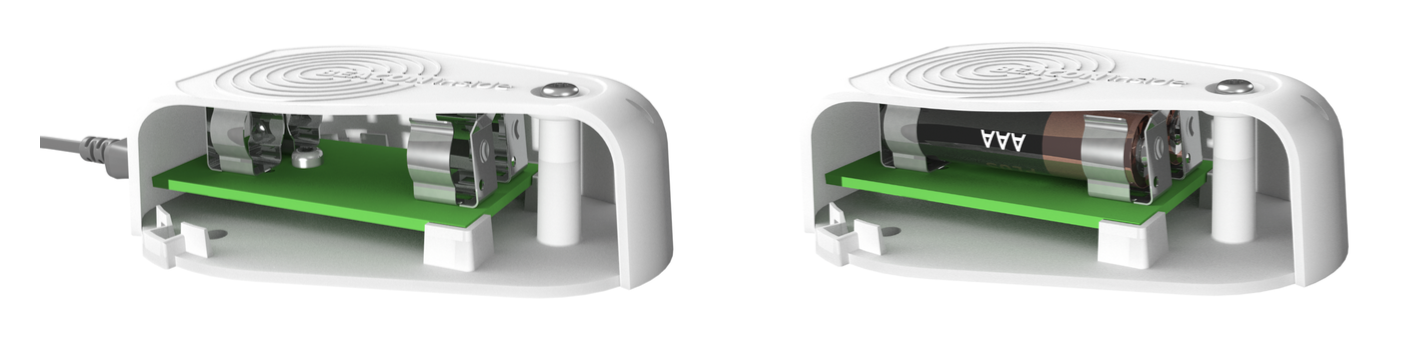
\includegraphics[width=0.6\textwidth]{figures/BEACONinside_beacons}
	\caption{A 3D picture of sectioned beacons \citep{binside:ds}.}
	\label{fig:bi:beacons}
\end{figure}

The beacons's size is 5.8\,cm\,$\times$\,7,96\,cm\,$\times$\,2.25\,cm. They can either be powered by two AAA~batteries to provide a lifespan of approximately one year, or by an external power supply over micro USB~\citep{binside:ds}.

The beacons are configurable with standard \ac{BLE} tools, like compatible smartphone apps. Such an app establishes a \ac{BLE} connection to the beacon. Each of the following configurable values can be accessed with a specific key. To configure the beacons an iOS app called \emph{LightBlue --- Bluetooth Low Energy}\footnote{Link to the LightBlue App in the iOS AppStore (last access: 21.04.2015) \url{https://itunes.apple.com/de/app/lightblue-bluetooth-low-energy/id557428110}} from a company named \emph{Punch Through Design LLC.}, recommended by BEACONinside is used. According to \citet{binside:ds}, the following values are configurable:
\begin{itemize}
  \item \textbf{\texttt{proximityUUID}:} For instance \texttt{F0018B9B-7509-4C31-A905-1A27D39C003C}
  \item \textbf{\texttt{major}:} A value between 1\,--\,65535
  \item \textbf{\texttt{minor}:} A value between 1\,--\,65535
  \item \textbf{\texttt{\acs{TX}-power level}:} It defines the power level which is used to transmit the beacons advertisement packages, i.e.\ the signals. It can either be 0\,dBm (default) which is the maximum power level, -6\,dBm or -23\,dBm which is the minimum power level.
  \item \textbf{\texttt{Advertising interval}:} Defines the time interval (100\,ms\,--\,10\,s) in which advertisements are sent. The default time interval is 400\,ms, configurable in steps of 625\,$\mu$s.
  \item \textbf{\texttt{Calibration value}:} To estimate the distance of the receiving device to the beacon a calibration step is necessary. The measured \acs{RSS} in a distance of 1m needs to be sent by the beacon with every advertisement. This value can be configured for each \texttt{Tx-power level}. The default is 65\,dBm for the 0dBm power level. It needs to be encoded as the 2' complement in hexadecimal (e.g.\ 65\,dBm = \text{0xBF}).
  \item \textbf{\texttt{Passkey}:} To set one of this configuration parameters the (6 digit) passkey must be entered. The beacons' default value is \texttt{555555}.
\end{itemize}

\noindent Additionally, the following read-only properties about the device and its state are provided~\citep{binside:ds}:
\begin{itemize}
  \item \textbf{\texttt{Device Name}:} The beacon's name consisting of \texttt{BEACON} and the latter three bytes of its \acs{MAC} address.
  \item \textbf{\texttt{Model Number}}
  \item \textbf{\texttt{Serial Number}}
  \item \textbf{\texttt{Hardware Revision Number}}
  \item \textbf{\texttt{Software Revision Number}}
  \item \textbf{\texttt{Manufacturer Name}}
  \item \textbf{\texttt{Battery Level}:} In percent.
  \item \textbf{\texttt{Temperature}:} The hardware's temperature in degrees Celsius.
\end{itemize}

\noindent To load the new values after changing the beacon's configuration, the beacon needs to be rebooted by setting a specific value. The beacon can also be reset to factory defaults~\citep{binside:ds}.

\subsection{Deployment and Calibration}
As mentioned before, the \ac{BLE} signal quality is heavily influenced by physical materials due to the fact that \ac{BLE} uses the 2.4\,GHz frequency. Especially, water which is a main part of the human body, attenuates the signal~\citep{apple:getting_started}. Thus, the beacons need to be carefully deployed. Ideally, they should be deployed in a manner, that most often the line between beacon and receiver is unobstructed. There should also be enough space around the beacon, that its signal can spread out. By deploying them carefully, the signal's attenuation and other effects like multi-path fading and shadowing can be reduced~\citep{apple:getting_started,IEEE:survey_wireless_indoor_pos}.

The next step is the calibration step. To be able to estimate the distance between smartphone and beacon a reference value is needed. The reference value, as mentioned before, is the measured \ac{RSS} in a distance of 1m to the beacon. The calibration value is configured on the beacon itself, which includes it in the sent advertisement together with its identifier.

According to \citet{apple:getting_started}, the smartphone needs to be positioned in 1m distance to the beacon in portrait mode with the device's top half uncovered. Then the \ac{RSSI} values were collected for at least 10s. Meanwhile, the user should slowly move the device on an $\approx$\,30\,cm line in front of the beacon, by maintaining distance and orientation. After collecting the values, the average value is calculated and configured on the beacon. It is advisable, to double check the device's estimated distance, after setting the calibration value. Due to the above mentioned problems, this needs to be repeated for every single beacon.

\section{API --- iOS 8.1}
After describing what beacons are and how they work, this section focuses on the receivers side, especially on the \acs{API} provided by Apple's iOS~8.1 platform. The \acf{CL} framework's \texttt{CLLocationManager} component provides two functionalities, called \emph{region monitoring} and \emph{beacon ranging} to receive a beacon's signals within an iOS app \citep{apple:ios_doc_cl}.

\subsection*{Region monitoring}
As the name already implies, the operating system monitors a specified region and notifies the application, when the user entered or left the region. This functionality is not restricted to regions established by beacons. It already existed long before, and monitors circular regions specified by a distance around a global position in longitude and latitude, e.g.\ a \acs{GPS} position.
iOS monitors the specified regions also if the application is in background mode or is currently not running. If the user enters or leaves a region, the application is launched by the \ac{OS}; for instance, to a notification to the user\citep{apple:wwdc_2012_bruins,apple:wwdc_2013_bruins,apple:ios_doc_cl}.

\subsection*{Proximity to a Beacon}
To continuously estimate the proximity to a beacon, ranging must be used. To enable that a \texttt{CLBeaconRegion} needs to be specified. The \texttt{CLBeaconRegion} object requires at least the beacon's \texttt{proximityUUID}. Furthermore, it is possible to specify a specific set of beacons, by adding the beacons' \texttt{major} identifier. Of course they have to share the same major identifier. By additionally providing a \texttt{minor} identifier, the framework searches only for one specific beacon~\citep{apple:wwdc_2013_bruins,apple:ios_doc_cl}.

After starting the search, the \texttt{CLLocationManager} starts to notify the before specified \texttt{delegate} object in a continuous manner after it received the first advertisement from a beacon, which it is supposed to range for. This means that the \texttt{CLLocationManager} does not call the \texttt{delegate} until it receives the first matching beacon advertisement. After the first call it continuously calls the delegate approximately every second regardless of whether it actually received a beacon's advertisement or not.

The \texttt{CLLocationManager} passes an array of \texttt{CLBeacon} objects to its delegate. Each of it represents one beacon. Table~\ref{tab:beaconExampleData} shows two example data sets, which the \texttt{CLLocationManager} passes to its delegate. Each data set contains four \texttt{CLBeacon} objects. The table's last entry represents a beacon, which is out of range.

\begin{table}
	\begin{tabular}{*{7}{c}}
time & proximityUUID & major & minor & proximity & accuracy & rssi \\
\hline
1.0400 & F0018B9B-\dots-1A27D39C003C & 21500 & 48945 & 2 & 1.2915 & -67\\
1.0400 & F0018B9B-\dots-1A27D39C003C & 39821 & 56686 & 2 & 5.9948 & -79\\
1.0400 & F0018B9B-\dots-1A27D39C003C & 41738 & 1201 & 3 & 6.8129 & -80\\
1.0400 & F0018B9B-\dots-1A27D39C003C & 38722 & 6270 & 3 & 7.7426 & -81\\
 & & & & & & \\
2.0387 & F0018B9B-\dots-1A27D39C003C & 21500 & 48945 & 2 & 1.4452 & -68\\
2.0387 & F0018B9B-\dots-1A27D39C003C & 39821 & 56686 & 3 & 5.5235 & -78\\
2.0387 & F0018B9B-\dots-1A27D39C003C & 41738 & 31201 & 3 & 6.8129 & -80\\
2.0387 & F0018B9B-\dots-1A27D39C003C & 38722 & 6270 & 0 & -1 & 0\\
\end{tabular}

	\caption{Two successive example datasets of \texttt{CLBeacon} objects passed by the\texttt{CLLocationManager} to the specified delegate.}
	\label{tab:beaconExampleData}
\end{table}

A \texttt{CLBeacon} object contains on one hand the beacon's identifiers, as described in Section~\ref{sec:beacon}. On the other hand, it contains three values, which express the beacons proximity in different ways.

\subsubsection*{\acs{RSSI} Property}
The \texttt{rssi} property, stores the \acl{RSS} measured in dBm. It expresses how strong the received signal is. As mentioned before, a beacons' advertisement time interval can be specified. Remember, the used beacons use send their advertisement per default every 400ms. The framework itself sticks to its $\approx$~1s time interval. It collects all received advertisements and calculates the average since the last reported \texttt{rssi} value. If a beacon's signal was received before, but not during the current time interval, its \texttt{rssi} value is 0 \citep{apple:wwdc_2013_bruins,apple:ios_doc_cl}.

\subsubsection*{Proximity Property}
The \texttt{proximity} property's value expresses the relative distance to a beacon. It can either be \texttt{unknown = 0}, \texttt{immediate = 1}, \texttt{near = 2}, or \texttt{far = 3}. The \texttt{unknown} state means, that the proximity could not be detected. One reason could be, that the beacon ranging just started but not enough advertisements were received. The \texttt{immediate} state ``represents a high level of confidence that the device is physically very close to the beacon''~\citep{apple:getting_started}. The \texttt{near} state is reported, if the user is in approximately 1~--~3m proximity to the beacon. Consequently, the \texttt{immediate} state is reported if the user is closer than $\approx$~1m and the state \texttt{far} is reported if the ``beacon device can be detected but the confidence in the accuracy is too low to determine either Near or Immediate''~\citep{apple:getting_started}. Hence, the estimated distance is larger than $\approx$~3m.

\subsubsection*{Accuracy Property}
The object's \texttt{accuracy} property actually expresses the proximity to a beacon in meters, but \citet{apple:ios_doc_cl} describes the property as follows:
\begin{quote}
  ``The accuracy of the proximity value, measured in meters from the beacon.
  [\dots]
  Indicates the one sigma horizontal accuracy in meters. Use this property to differentiate between beacons with the same proximity value. Do not use it to identify a precise location for the beacon. Accuracy values may fluctuate due to RF interference.''\citep{apple:ios_doc_cl}
\end{quote}
Thus, I first interpreted this description as the error of the \texttt{proximity} property's value, measured in meters. But, this makes of course not much sense, because the \texttt{proximity} value stores a relative value, which already implies that the user's proximity to the beacon is in a certain range.

\begin{equation} \label{eq:rssiToDistanceCalc}
	d = 10^{-\frac{RSSI + A}{10 * n}}
\end{equation}

According to \citet{wang:bt_pos}, the distance $d$, between an iBeacon and a smartphone, which depends on the \acl{RSS}, can be calculated with the formula shown in equation~\ref{eq:rssiToDistanceCalc}, where $A$ is the \acs{RSSI} value at a distance of 1m, and $n$ an environmental constant. To prove the assumption, that the \texttt{accuracy} value is actually the distance, test measurements for certain reference distances were performed. The measurements were taken outdoor with \ac{LOS} between beacon and smartphone in order to have the signal's quality as less impacted by physical materials as possible. After collecting the \acs{RSSI} and \texttt{accuracy} values of 60 measurements for each reference distance the data set was sorted according their \texttt{rssi} values. Then the \texttt{accuracy} value's average per \texttt{rssi} was calculated. Afterwards, the above mentioned formula shown in equation~\ref{eq:rssiToDistanceCalc} was used to calculate the distance for each measured \texttt{rssi} value. During the measurements, the beacon's calibration value was set to 65dBm; thus, $A = 65\text{dBm}$. To approximate the \texttt{CLBeacon} object's \texttt{accuracy} property best, an environmental constant of $n = 2.1$ was used, which is similar to the one used by \citet{wang:bt_pos}.

Figure~\ref{fig:eval_accuracy_vs_distance} illustrates the result and the fact, that the \texttt{CLBeacon} object's \texttt{accuracy} property is the estimated distance, between beacon and smartphone. Additionally, it implicitly depicts, that the unit dB is a logarithmic unit.

\begin{figure}
  \begin{tikzpicture}
    \begin{axis}[width=0.9\textwidth, height=0.45\textheight,
        xlabel={\acl{RSS} (dBm)},
        ylabel={Estimated Distance (m)},
        legend pos=north west,
        legend entries={measurement, avg.\ \texttt{accuracy} per \texttt{rssi}, $d = 10^{-\frac{RSS + 65}{10 * 2.1}}$},
      grid = major,
      x dir=reverse, ymin=0]
      \addplot [only marks, mark=x] table[col sep=semicolon, x=rssi, y=accuracy] {csv/2014-10-15_hoehenweg/all.csv};
      \addplot [red, mark=triangle*, mark size=3pt] table[col sep=semicolon, x=rssi, y=avgAccuracy] {csv/2014-10-15_hoehenweg/all_avg_accuracy_per_rssi.csv};
      \addplot[blue, domain=-55:-95, samples=100]{10^(-(x+65)/(10*2.1))};
  \end{axis}
\end{tikzpicture}

	\caption{Dependency of the \texttt{CLBeacon} object's \texttt{rssi} and \texttt{accuracy} property. Proves that the \texttt{CLBeacon} object's \texttt{accuracy} is the estimated distance between smartphone and beacon because $d$ is the estimated distance depending on the \ac{RSS} according to \citet{wang:bt_pos,kotanen:exp_local_pos_bt}.}
	\label{fig:eval_accuracy_vs_distance}
\end{figure}

% Wenn es genauigkeit wäre müsste es an den Übergängen von klein zu groß ja auch einen sichtbaren unterschied geben


\section{Evaluation}\label{sec:beacon_eval}
After explaining how beacon advertisements can be received within an iOS app and which data can be accessed, this Chapter evaluates the \texttt{CLBeacon} object's data especially the \texttt{accuracy} property's values, which are the ones used by the solution's algorithm.

First, the distance estimations's quality i.e.\ its error in different situations is evaluated. Afterwards, the result of an experiment which uses only multilateration to determine a user's position is presented.

\subsection{Distance Estimation}
The measured distances provided by the \texttt{CLBeacon} object's \texttt{accuracy} property varies in dynamic, but also in steady and unobstructed environments, due to the following reasons.

%\subsubsection*{Dependency of \texttt{rssi} and \texttt{accuracy}}
\subsubsection*{Filtering}
The first reason is, that the measured \ac{RSS} is not directly used to calculate the \texttt{accuracy} value. The \acl{CL} framework seems to apply a filter to the \texttt{CLBeacon} object's values. To test this the \texttt{CLBeacon} object's properties were recorded over time. During the test the smartphone was positioned with a distance of 2\,m to the beacon. The data recording started directly after positioning the smartphone. Figure~\ref{fig:beacon_eval_accuracy-rssi} illustrates the recorded \texttt{rssi} values and their corresponding \texttt{accuracy} values over time. The graph shows, that the \texttt{accuracy} values slowly converge against the actual distance of 2\,m. Furthermore, it shows that outliers in the \texttt{rssi} property do not have a direct impact on the estimated distance. Consequently, it is very likely that \ac{CL} filters the values provided by the \texttt{CLBeacon} object. Furthermore, it shows that the \texttt{accuracy}, i.e.\ estimated distance, not only depends on the corresponding \texttt{rssi} value.

\begin{figure}
	\begin{tikzpicture}
    \begin{axis}[width=0.9\textwidth, height=0.45\textheight,
      xlabel={Time (sec)},
      axis y line*=left,
      ylabel={Estimated Distance (m)},
        legend pos=south west,
      legend entries={\texttt{accuracy}, ref.\ distance}]
      \addplot [blue, mark=x] table[col sep=semicolon, x=time, y=accuracy] {csv/2014-10-27_htwg_f007/04_2m.csv};
      \addplot [black, dashed, domain=0:54, samples=2]{2};\label{distance}
  \end{axis}
  \pgfplotsset{every axis y label/.append style={rotate=180, yshift=15cm}}
  \begin{axis}[width=0.9\textwidth, height=0.45\textheight,
    axis y line*=right,
    ylabel={\acl{RSS} (dBm)},
    hide x axis,
    y dir=reverse,
    legend entries={\texttt{rssi}}]
    \addplot [red, mark=*] table[col sep=semicolon, x=time, y=rssi] {csv/2014-10-27_htwg_f007/04_2m.csv};
  \end{axis}
\end{tikzpicture}

	\caption {Dependency of the \texttt{CLBeacon} object's \texttt{accuracy} and \texttt{rssi} property over time with an actual distance of 2\,m.}
	\label{fig:beacon_eval_accuracy-rssi}
\end{figure}

\subsubsection*{Attitude \& Obstacles}
The second reason is the device's attitude relative to the beacon. Figure~\ref{fig:beacon_eval_situations} illustrates the impact on the estimated distance and the \ac{RSS} in typical situations.
During the experiment the actual distance between smartphone and beacon was 1\,m. The measurements were taken indoor. The values shown in Figure~\ref{fig:beacon_eval_situations} are average values. For each situation 60\,--\,100 values were recorded.\newline

\textbf{Situations:}
\begin{itemize}
  \item \emph{(1)} Horizontal iPhone in front of vertical beacon with \acs{LOS}.
  \item \emph{(2)} Horizontal iPhone sideways to vertical beacon with \acs{LOS}.
  \item \emph{(3)} Horizontal iPhone with angle of $45~\circ$ below vertical beacon with \acs{LOS}.
  \item \emph{(4)} Vertical iPhone in front of vertical beacon with \acs{LOS}.
  \item \emph{(5)} Horizontal iPhone in front of horizontal beacon with \acs{LOS}.
  \item \emph{(6)} Horizontal iPhone in front of vertical Beacon with person in between.
  \item \emph{(7)} Horizontal backwards turned iPhone in front of vertical Beacon with \acs{LOS}.
  \item \emph{(8)} Horizontal backwards turned iPhone in front of vertical Beacon with person in between.
  \item \emph{(9)} Horizontal iPhone in front of vertical Beacon with 30 cm ferro concrete wall in between.
\end{itemize}

\noindent Situation 1, 2, 5 and 7 shows, that if the iPhone is horizontal in front of, or sideways of the vertical beacon with \acs{LOS}, the \acs{RSS} attenuation is the lowest. In contrast, if the beacon's signals are received with a different angle as shown by situation 3 and 4 the attenuation increases.

Furthermore, Figure~\ref{fig:beacon_eval_accuracy-rssi} depicts the third reason, which is static obstacles such as walls or the user's own body. A human body between the phone and a beacon, shown in situation 6 and 8, has a much higher impact. The estimated distance increases by approximately 3\,m. Whereas a ferro concrete 30\,cm wall, shown in situation 9, drastically impacts the distance. The phone estimates a distance of 9\,m instead of 1\,m.

The above illustrated scenarios are very common. The problem is, that without knowing its own exact position, the beacons attitude, and the positions of all obstacles one cannot distinguish, whether an estimated distance is impacted by the attitude, a wall, or a person.

\begin{figure}
	\subfloat[The average estimated distance in different situations.]{
  \begin{tikzpicture}
    \begin{axis}[width=0.45\textwidth, height=0.35\textheight,
        xlabel={Situation},
        ylabel={Estimated Distance (m)},
        xtick=data,
        legend entries={\texttt{accuracy}},
        legend pos = north west,
      grid = major]
      \addplot [only marks, mark=*] table[col sep=semicolon, x=measurement, y=accuracy] {csv/2014-10-27_htwg_fk034_angles/all_avg.csv};
  \end{axis}
\end{tikzpicture}
}
\subfloat[The average \acs{RSS} in different situations.]{
  \begin{tikzpicture}
    \begin{axis}[width=0.45\textwidth, height=0.35\textheight,
        xlabel={Situation},
        ylabel={\acl{RSS} (dBm)},
        y dir=reverse,
        xtick=data,
        legend entries={\texttt{rssi}},
        legend pos = north west,
      grid = major]
      \addplot [only marks, mark=*] table[col sep=semicolon, x=measurement, y=rssi] {csv/2014-10-27_htwg_fk034_angles/all_avg.csv};
  \end{axis}
\end{tikzpicture}
}

	\caption {The impact on the beacon signal's quality, i.e.\ the \texttt{CLBeacon} object's \texttt{accuracy} and \texttt{rssi} values in different situations, such as obstacles between smartphone and beacon, and the smartphone's orientation relative to a beacon. For each value 60\,--\,100 measurements were recorded with an actual distance of 1\,m.}
	\label{fig:beacon_eval_situations}
\end{figure}


\subsubsection*{Distribution and Error}
To depict that the estimated distance also varies in steady unobstructed environments with \acs{LOS}, the \texttt{accuracy} values for different reference distances in different environments were measured. For each reference distance 60 values were recorded. For each environment the used beacons were calibrated.

Figure~\ref{fig:beacon_dispersion_outdoor} illustrates the collected \texttt{accuracy} values measured at 1, 2, \ldots, 5, 10, \ldots, 30\,m distance to the beacon. The measurements were taken outdoor with \acl{LOS} between the beacon and the smartphone.

The graph shows, that the average \texttt{accuracy} measured at 1\,--\,4\,m distance is very close to the actual distance. It also shows that the value's distribution for these distances is very low. For distances $\geq$\,5\,m, the spreading increases and varies between small and large. Thus, it is not correlated to the reference distance.

As mentioned before, the beacons manufacturer claims a maximum range of 40\,m. In this scenario the beacon's signals could be received up to a distance of 42\,m.

The exact same experiment was repeated in an indoor environment. The results are depicted in Figure~\ref{fig:beacon_dispersion_f-cellar}. Also in this case the average \texttt{accuracy} comes very close to the actual distance with a very low spreading for the first 4 distances. At 5\,m the distribution and error increases and decreases, too.

Interestingly, the value's distribution starts to decrease between 10\,--\,30\,m from very large to a much smaller value. At the same time the error grows because the smartphone estimates a very small distance due to the \ac{RSS}; whereas, the actual distance is very large. The assumed reason is the test environment's construction form. The measurements were recorded in a straight, long, but narrow corridor in a basement. There are multiple doors made of steel on both sides of the wall, that maybe caused reflections.

The depicted measurements in Figure~\ref{fig:beacon_dispersion_f007} were recorded in an $\approx$\,15\,m long and 8\,--\,11\,m wide lecture hall. It shows, that also the first few meters on average are matching best, but it also depicts, that there are sometimes huge differences in the estimated distance at the same position.

\begin{figure}
	\subfloat[Measured outdoor]{
  \begin{tikzpicture}
    \begin{axis}[trim axis left, trim axis right, width=0.45\textwidth, height=0.45\textheight,
        xlabel={Reference Distance (m)},
        ylabel={Estimated Distance (m)},
        legend pos=north west,
        legend entries={\texttt{accuracy}, avg. \texttt{accuracy}},
        grid = major]
      \addplot [only marks, mark=x] table[col sep=semicolon, x=proximityRef, y=accuracy] {csv/2014-10-15_hoehenweg/all.csv};
      \addplot [red, only marks, mark=triangle*, mark size=3pt] table[col sep=semicolon, x=proximityRef, y=avgAccuracy] {csv/2014-10-15_hoehenweg/avg_all.csv};
      \addplot [black, dashed, domain=0:30, samples=2]{x};
  \end{axis}
\end{tikzpicture}
\label{fig:beacon_dispersion_outdoor}
}
\subfloat[Measured in basement (HTWG-KN F)]{
  \begin{tikzpicture}
    \begin{axis}[width=0.45\textwidth, height=0.45\textheight,
        xlabel={Reference Distance (m)},
        ylabel={Estimated Distance (m)},
        legend pos=north west,
        legend entries={\texttt{accuracy}, avg. \texttt{accuracy}},
        grid = major]
      \addplot [only marks, mark=x] table[col sep=semicolon, x=proximityRef, y=accuracy] {csv/2014-10-15_htwg_keller_f/all.csv};
      \addplot [red, only marks, mark=triangle*, mark size=3pt] table[col sep=semicolon, x=proximityRef, y=avgAccuracy] {csv/2014-10-15_htwg_keller_f/all_avg_accuracy_per_proximity.csv};
      \addplot [black, dashed, domain=0:30, samples=2]{x};
  \end{axis}
\end{tikzpicture}
\label{fig:beacon_dispersion_f-cellar}
}

\subfloat[Measured in lecture hall (HTWG-KN F007)]{
\begin{tikzpicture}
    \begin{axis}[width=0.45\textwidth, height=0.45\textheight,
        xlabel={Reference Distance (m)},
        ylabel={Estimated Distance (m)},
        legend pos=north west,
        legend entries={accuracy, avg. accuracy},
        legend entries={\texttt{accuracy}, avg. \texttt{accuracy}},
        grid = major]
      \addplot [only marks, mark=x] table[col sep=semicolon, x=proximityRef, y=accuracy] {csv/2014-10-27_htwg_f007/all.csv};
      \addplot [red, only marks, mark=triangle*, mark size=3pt] table[col sep=semicolon, x=proximityRef, y=avgAccuracy] {csv/2014-10-27_htwg_f007/all_avg_accuracy_per_proximity.csv};
      \addplot [black, dashed, domain=0:14.5, samples=2]{x};
  \end{axis}
\end{tikzpicture}
\label{fig:beacon_dispersion_f007}
}

	\caption{The distribution of the estimated distances, i.e.\ the measured \texttt{accuracy} values, depending on the actual distance and the environment.}
	\label{fig:beacon_dispersion}
\end{figure}

% paragraph{Uncertainty}
As mentioned in Section~\ref{sec:fund_loc}, it is necessary to know the uncertainty of a measurement to implement a \acl{PF}. Thus, the distance estimation's uncertainty were determined based on the data shown in Figure~\ref{fig:beacon_dispersion_outdoor} and \ref{fig:beacon_dispersion_f007}. The Gaussian's parameters to model the distance estimation's uncertainty are depicted in Figure~\ref{fig:beacon_eval_ndf}. The two dashed straight lines show the linear function that approximates the standard deviation $\sigma$ depending on the mean $\mu$ best.

\begin{figure}
	\begin{tikzpicture}
    \begin{axis}[trim axis left, trim axis right, width=0.9\textwidth, height=0.45\textheight,
        %title={Normal Distribution Function parameters},
        xlabel={Mean $\mu$ (m)},
        ylabel={Standard deviation $\sigma$ (m)},
        legend pos=south east,
        legend entries={outdoor, $f(\mu)=0.3286 \cdot \mu + 0.8379$, indoor (HTWG-KN F007), $f(\mu)=0.3131 \cdot \mu + 0.0051$},
      grid = major]
      \addplot [red, mark=*] table[col sep=semicolon, x=mu_distance, y=sigma_distance] {csv/2014-10-15_hoehenweg/ndf_parameters.csv};
      \addplot [red, dashed, domain=0:30, samples=2]{0.3286*x+0.8379};
      \addplot [blue, mark=*] table[col sep=semicolon, x=mu_distance, y=sigma_distance] {csv/2014-10-27_htwg_f007/ndf_parameters.csv};
      \addplot [blue, dashed, domain=0:30, samples=2]{0.3131*x+0.0051};
  \end{axis}
\end{tikzpicture}

	\caption{The distance estimations' uncertainties, modeled as Gaussians, depending on the actual distance. Additionally, the uncertainties were approximated by linear regression.}
	\label{fig:beacon_eval_ndf}
\end{figure}


\subsection{Multilateration}
After evaluating the distance estimation's quality of one beacon, some beacons were deployed in a lecture hall to get a better feeling of how good the distance estimation actually works. On one hand, the goal was to visualize the estimated distances on a map, to proof their plausibility, and on the other hand, to test if indoor self-localization with smartphones is possible by just using iBeacons without integrating additional sensor data.

As already mentioned in Section~\ref{sec:fund_trilateration}, \emph{multilateration} is a method to estimate a position by using the distances to several transmitters. If one uses only one sender then the receiver's position is somewhere on a circle around the transmitter with the estimated distance as radius of the circle.
By using two tranmitters $t_1$ and $t_2$, the two circles around the transmitters can have zero, one or two intersections, if the position of $t_1 \neq t_2$. Thus, the receiver's position must be at one of the circles' intersections.
By adding a third transmitter $t_3$ the three circles have either no or exactly one, common intersection point, which is the receiver's position. This applies also to more than three transmitters.

To be able to use the implementation with variable transmitter count the \emph{Least Square} method to determine the receiver's position was used. Another advantage is that the least square method can also estimate a position if no common intersection point exists.

For the experiment the same lecture hall as before was used. There, four beacons were positioned. Then the test device, which is an iPhone\,5S, was used to recorded the received beacon identifiers with their corresponding estimated distances, i.e.\ the \texttt{accuracy} values, provided by \acs{CL}, during a test walk on a defined path.

To visualize the estimated distances to the beacons and the device's estimated position, i.e.\ the walked path, I wrote a small Python program. Figure~\ref{fig:beacon_eval_multilat} shows four screenshots of the program's output. Each of it shows a map, which shows the lecture hall walls in grey. The white space in the hall is free space. The filled small blue circles next to the walls are the four beacons. The big blue circles, are the circles around the beacons, where the radius represents the estimated distance to the beacons. The test person walked on the green tetragon, beginning at the bottom right corner in counter clockwise direction by holding the test device in front of oneself. The beacons were positioned at approximately the same height as the device in the test person's hand. The red line shows the estimated path.

The first screenshot depicted in Figure~\ref{fig:beacon_eval_multilat_1} shows, that the estimated distance sometimes is completely wrong, as shown by the blue circle around the top-right beacon. It also shows that the estimated position is somewhere several meters outside of the lecture hall. The second screenshot shows, that the distance to the top-right beacon shrinks, but the one to the top-left massively grows. The distances to the other two beacons seem to be plausible. Figure~\ref{fig:beacon_eval_multilat_3} shows a plausible position. It also shows, that in this step the beacon's signal, positioned at the bottom-right corner, was not received. The last screenshot shows also a more or less plausible position. The distances, except the one to the beacon, positioned at the bottom-left corner, seem to be plausible.

\begin{figure}
  \subfloat[]{
  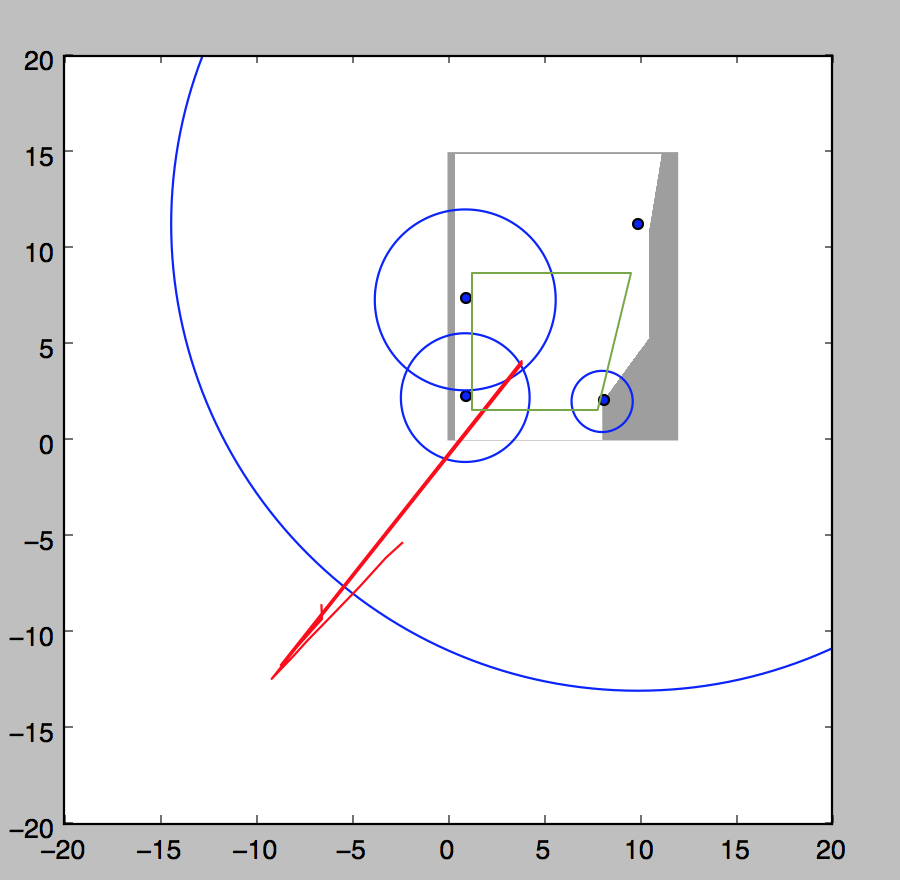
\includegraphics[width=0.45\textwidth]{figures/multilat_1}
  \label{fig:beacon_eval_multilat_1}
}
\subfloat[]{
  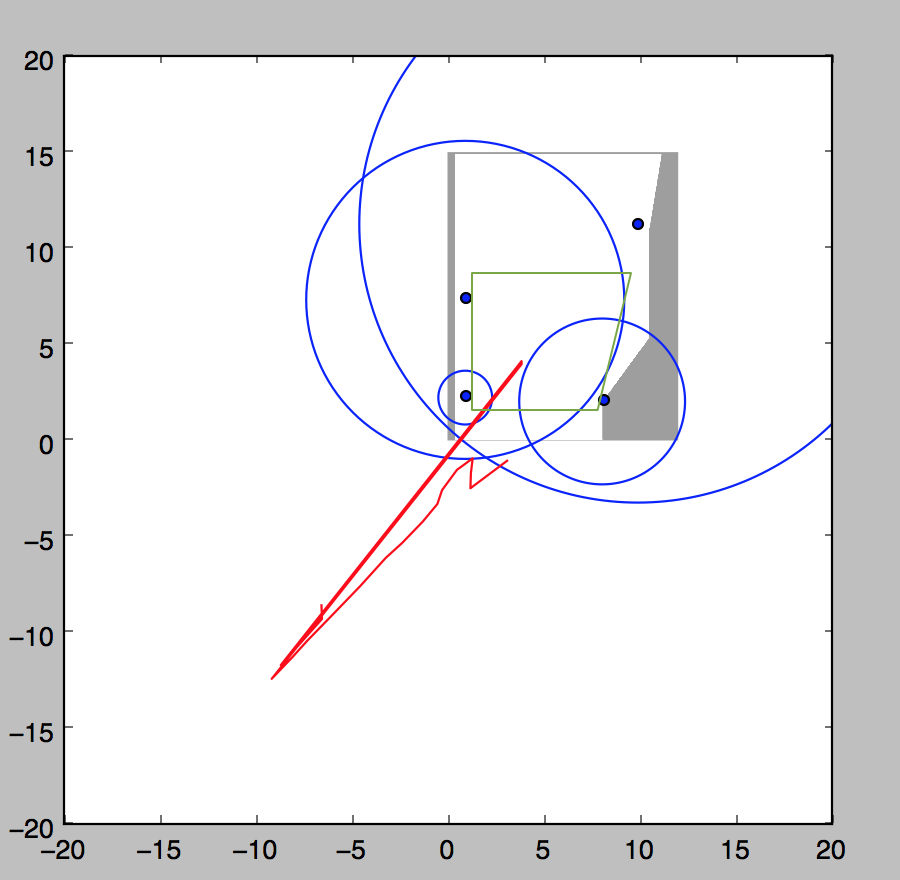
\includegraphics[width=0.45\textwidth]{figures/multilat_2}
}

\subfloat[]{
  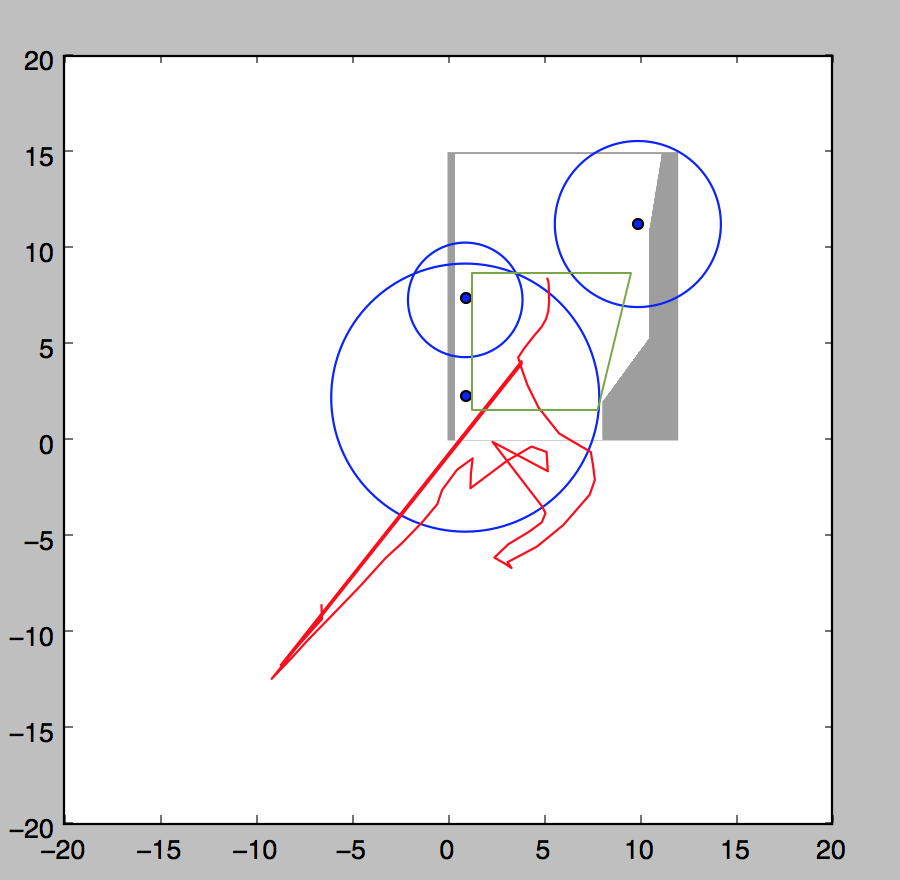
\includegraphics[width=0.45\textwidth]{figures/multilat_3}
  \label{fig:beacon_eval_multilat_3}
}
\subfloat[]{
  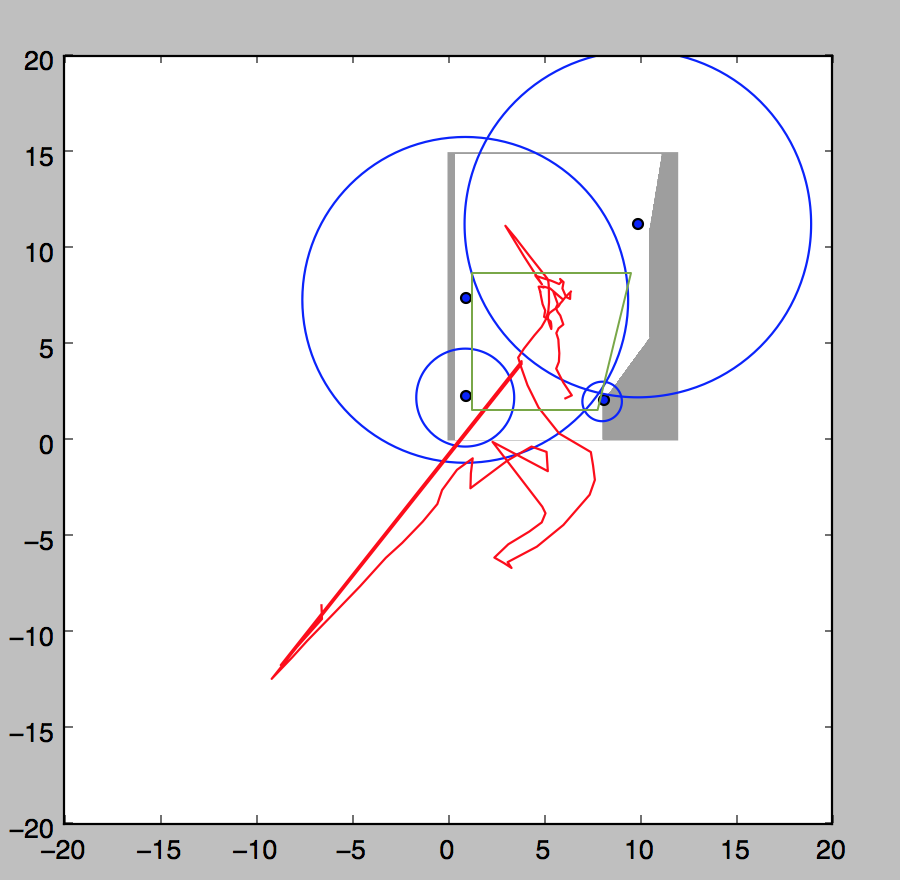
\includegraphics[width=0.45\textwidth]{figures/multilat_4}
}

  \caption{Four successive screenshots of the indoor self-localization experiment in a lecture hall (HTWG-KN F007) using multilateration. The screenshots show a map of the lecture hall, the walked path in green, the beacons as blue filled circles and their estimated distances as large blue circles. The red line depicts the estimated path.}
  \label{fig:beacon_eval_multilat}
\end{figure}

The experiment was repeated with the same setting and recorded data, but only used those beacon signals where the \texttt{accuracy} was $<$\,5\,m. Signals with larger estimated distances were ignored. Figure~\ref{fig:beacon_eval_multilat_less5m} shows the result. The estimated path actually is inside of the lecture hall. It is not possible to determine that the test person walked on the green path, but ignoring values more than 5\,m seems to improve the location estimation.

\begin{figure}
	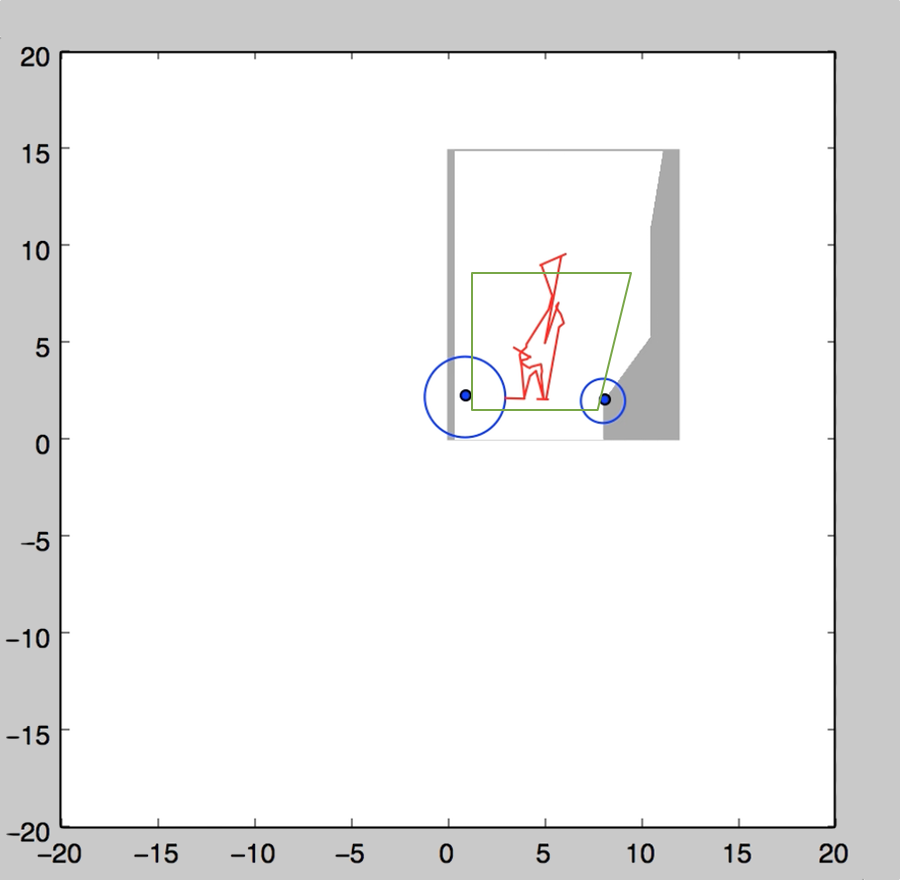
\includegraphics[width=0.45\textwidth]{figures/multilat_less5m}
	\caption{Screenshots of the indoor self-localization experiment in a lecture hall (HTWG-KN F007) using multilateration by only ignoring estimated distances more than 5\,m. The screenshots show a map of the lecture hall, the walked path in green, the beacons as blue filled circles and their estimated distances as large blue circles. The red line depicts the estimated path.}
	\label{fig:beacon_eval_multilat_less5m}
\end{figure}

This experiment shows, that due to the very unreliable distance estimations the beacons' signals must be heavily influenced. It also shows that pure multilateration, without filtering the data and without integrating additional data sources, is not sufficient for indoor self-localization.

\subsection{Summary}
The results show, that the distance estimation not just depend on the beacons calibration, it also depends on the buildings construction form, the phones relative orientation to the beacons, and the obstacles in between.

It also points out, that the \texttt{CLBeacon}'s \texttt{accuracy} i.e.\ the estimated distance, comes very close to the actual distance up to 4\,--\,5\,m with \acs{LOS}. Larger distances cause a much higher spreading, and thus, a larger error. Physical material like humans and walls cause attenuation, which results in a larger distance estimation than it actually is. Besides that, the estimated distance is sometimes very small compared to the actual distance.

To conclude, the estimated distances are very unreliable. Thus, their plausibility should be proven to filter the measurements. But due to the fact, that the validity cannot be proven without knowing the exact position of the receiver and the properties of all other influencing factors, which is not a trivial problem in large buildings, the only one possible improvement that could be applied, is to ignore beacons with an estimated distance larger than 5~meters. This solves of course not the problem with those beacons, which appear to be closer than they actually are. But from my point of view no real solution exists to solve this problem.
\chapter{Built-in Sensors} \label{chap:sensors}

This chapter describes first the suitable built-in sensors of the current smartphone generation. Afterwards, it provides an overview of the appropriate \acsp{API} to access either raw or processed sensor data. Finally, the data provided by the sensors' \acsp{API} is evaluated.


\section{Built-in Sensors}
Todays smartphones contain several sensors to provide applications the possibility to measure physical properties of the smartphone's environment. By measuring environmental properties applications can process and react on them. This section gives an overview of available sensors of the latest smartphone generation that are suitable for this project. It also describes the physical properties that can be measured by them and their functionality.


\paragraph{Magnetometer}
Today, most smartphones have a built-in magnetometer to measure the strength and direction of a magnetic field. Typically, the magnetometer is built with at least one hall sensor which usually measures the magnetic field, i.e.\ the magnetic flux density, in micro teslas. For instance, Apple's iPhones includes a three-axis magnetometer; thus, it is able to determine the orientation in three-dimensional space, which is, for example being used, by the digital compass \citep{apple:wwdc_2012_pham,apple:ios_doc_cm}.


\paragraph{Accelerometer}
The accelerometer, which is also implemented in most smartphones, measures the acceleration applied to the device. The measured acceleration is the gravity plus the acceleration that the user applies to the device, measured in $\frac{m}{s^2}$. Thus, the measured acceleration is 1\,g\,=\,9.81\,$\frac{m}{s^2}$ if the device is stationary, i.e.\ no user acceleration is applied to the device. Typically, smartphones include a three-axis accelerometer to measure the acceleration along the three spatial axis to determine for example the device's tip and tilt \citep{apple:wwdc_2012_pham,apple:ios_doc_cm}.


\paragraph{Gyroscope}
Modern smartphones usually include a three-axis gyroscope to measure the rotation rate along the device's spatial axis. Rotation rate is measured in $\frac{rad}{s}$. Thus, the gyroscope can be used to determine the device's attitude. Like every sensor data, the gyroscope's measurements include some bias. Hence, determining the device's attitude with the raw gyroscope measurements includes a growing drift over time \citep{apple:wwdc_2012_pham,apple:ios_doc_cm}.


\paragraph{Barometer}
Some of the latest smartphones also include a barometer to measure air pressure. It is measured in $kilo pascals$. Thus, the relative change in altitude can be calculated. The barometer can be used for hiking apps, to determine the change in altitude for example \citep{apple:ios_doc_cm}.


\section{\acsp{API} --- iOS\,8.1}
To use the sensors within an application running on the device the \ac{OS} provides different \acp{API}. As mentioned before, the raw sensor data usually include some bias; for instance, the device's hardware biases the measured magnetic field. Apple's \ac{API} provides the possibility for all mentioned sensors, to access either raw sensor data including bias, or already filtered and processed data with less bias. This section provides an overview of the suitable higher level \acsp{API} with focus on Apple's iOS\,8.1 platform.


\paragraph{Motion Processing}
With the iPhone\,5S Apple introduced in 2013 a motion coprocessor, called M7. The latest iPhone, iPhone\,6 / iPhone\,6\,Plus, contains an improved version named M8, with improved accuracy. Additionally, it includes a barometer, which is processed by the motion coprocessor. The key features of the \ac{CM} framework and the motion coprocessor is sensor fusion, energy efficiency, and motion awareness, over the past seven days \citep{apple:wwdc_2014_pham}.

\ac{CM} implements algorithms to filter and combine the input of multiple sensors. Thus, the \acsp{API} can provide more accurate results for values such as the device's attitude. Together with the motion coprocessor it can offer more convenient interfaces to developers with already processed data, such as step counting and motion activity classification \citep{apple:wwdc_2014_pham}.

Earlier iPhones used their \acs{CPU} to gather and process sensor data, which is very energy consuming and inefficient, because it eats up a lot of \acs{CPU} time. According to \citet{apple:wwdc_2012_pham}, one of Apple's \ac{CM} engineers, the motion coprocessor is very energy efficient. He mentions, that the energy consumption of 24\,hours motion processing, e.g.\ motion activity classification, or the pedometer, is equal to a three minute FaceTime\footnote{FaceTime is Apple's video telephony application.} call.

Motion awareness gives applications the possibility to query the user's motion data for the past seven days.

\paragraph{Push and Pull Interface}
The following \acsp{API} provide to types of interfaces.

The \emph{push} interface continuously provides the application with new sensor data, usually within a certain time interval. To do so, the developer needs to provide and register a callback function. This function gets passed the new data.

The \emph{pull} interface is designed to query historical data within a specified range of time; for instance, the past seven days. According to \citet{apple:wwdc_2014_pham}, querying historical data is more accurate than the data provided via the push interface, because the filters can operate better on a larger data set. They also mention, that some values are adjusted, i.e.\ they adapt to the user's behavior over time; for instance, the pedometers stride estimation.

Both interfaces provide their data asynchronously to the developer's application.

\subsection{MotionActivity}
Apple's \texttt{CMMotionActivityManager}, which is part of the \ac{CM} framework, is able to detect and classify different activities, such as walking, running, cycling, etc. For the activity detection and classification the motion coprocessor is used together with the accelerometer \citep{apple:wwdc_2014_pham}.

As mentioned before, the \ac{CM} framework's MotionActivity \acsp{API} provides a push interface to receive motion activity changes, and a pull interface to query historical data between two dates. Both \acsp{API} are reporting every single change in motion activity, that was detected.

Table~\ref{tab:motionActivityScenarios} shows an overview of the different motion activities and illustrates some example scenarios. The states \texttt{walking}, \texttt{running}, \texttt{automotive}, \texttt{cycling}, and \texttt{unknown} are mutually exclusive motion activity types, whereas \texttt{stationary} is not mutually exclusive to the other types.

\begin{table}
	\begin{tabular}{l|c|ccccc}
Device scenarios & stationary & walking & running & automotive & cycling & unknown \\
\hline
On a table & \textbf{true} & false & false & false & false & false\\
Person checking email & false & false & false & false & false & false\\
Person walking & false & \textbf{true} & false & false & false & false\\
In idling vehicle & \textbf{true} & false & false & \textbf{true} & false & false\\
In moving vehicle & false & false & false & \textbf{true} & false & false\\
After reboot & false & false & false & false & false & \textbf{true}
\end{tabular}

	\caption{Example scenarios illustrating the \texttt{CMMotionActivity} object's activity classification \citep{apple:wwdc_2014_pham}.}
	\label{tab:motionActivityScenarios}
\end{table}


\noindent Thus,
\begin{itemize}
  \item a device lying \textbf{on a table} does not move; hence, it is stationary.
  \item a \textbf{person checking email}  usually does not hold its smartphone completely steady.
  \item a \textbf{person walking} can be detected across body location.
  \item in a \textbf{moving vehicle} the state is automotive.
  \item in an \textbf{idling vehicle}, e.g.\ in front of a stop sign, the state is stationary and automotive at the same time. The device needs to be mounted in car.

  \item immediate after a \textbf{reboot} the device's state is unknown because it first needs to collect some data to determine its real state.
\end{itemize}

\noindent As mentioned by \citet{apple:wwdc_2014_pham}, the \texttt{CMMotionActivityManager} has some latency depending on the activity and its location. For example, if a person is walking and holds the device in hand, it takes $\approx$\,5\,--\,10\,s to detect walking. If it is carried in a pocket it takes only $\approx$\,3\,--\,5\,s. To detect walking takes relatively long compared to the running state. Running can be detected within a couple of steps. According to \citet{apple:wwdc_2014_pham} one reason is that they can assume, that running persons does not check their emails or Facebook messages at the same time. If the smartphone is mounted in a car, the driving state can also be detected very fast. They also mention that the cycling state is very difficult to detect.

Another important point is the accuracy across body location. They point out, that the average accuracy across body location is always the same.

Every \texttt{CMMotionActivity} object which is reported to the application includes a \texttt{confidence} property. Confidence is measured at three different levels: \texttt{low\,=\,0}, \texttt{medium\,=\,1}, and \texttt{high\,=\,2}. Thus, the more confident the \texttt{CMMotionActivityManager} is about a motion activity state the higher the confidence value. Usually, it increases over time if the activity type does not change \citep{apple:wwdc_2014_pham,apple:ios_doc_cm}.


\subsection{Pedometer}
\begin{table}
	\begin{tabular}{l|*{4}{l}}
timestamp & startDate & endDate & distance & steps\\
\hline
9.3564 & 0.0019 & 9.2981 & 4.1351 & 7\\
14.4272 & 0.0019 & 11.8354 & 4.1351 & 7\\
14.4357 & 0.0019 & 14.3802 & 9.0606 & 15\\
16.9566 & 0.0019 & 16.9193 & 9.7806 & 16\\
22.0541 & 0.0019 & 19.4658 & 9.7806 & 16\\
22.0553 & 0.0019 & 22.0038 & 13.5247 & 22\\
24.6033 & 0.0019 & 24.5478 & 14.2447 & 23\\
29.6747 & 0.0019 & 27.0876 & 14.2447 & 23\\
29.6754 & 0.0019 & 29.6292 & 18.5546 & 30\\
32.2152 & 0.0019 & 32.1722 & 19.2546 & 31\\
\end{tabular}

	\caption{Recorded pedometer example data with additional timestamp. Remark: To simplify the table, relative values for timestamp, startDate and endDate are used instead of the absolute timestamps. The \emph{timestamp} column is actually not part of the \texttt{CMPedometerData}. Additionally all values, except the steps, are truncated.}
	\label{tab:pedometerExampleData}
\end{table}

The pedometer's \acs{API} is a component of Apple's \acs{CM} framework. It provides the distance a person traveled over time in meters. The iPhone needs to be equipped with a motion coprocessor\footnote{Note: iPads with motion coprocessor do not provide step counting and distance estimation.}. The motion coprocessor processes the accelerometer's data to count a person's steps and to estimate the person's stride length. The stride estimation adapts over time. Thus, the more often the pedometer is used the better the accuracy \citep{apple:wwdc_2014_pham}. According to \citet{apple:wwdc_2014_pham}, the pedometer has a consistent performance and accuracy across the phone's body location.

As mentioned before, there are two different interfaces to request the pedometer data. Via the pull interface the application can ask the pedometer component for the distance a person traveled by passing a start and end date. The second possibility is the push interface. With it the application can register a callback function to receive updates while the person is walking. If the user is walking or running the function is called every $\approx$\,2.5\,s, assuming the motion processor detects the taken steps. If it does not detect steps the handler is not called. The received steps and distances are the cumulative step count and distance since the start date, which is for all successive \texttt{CMPedometerData} objects the same \citep{apple:wwdc_2014_pham}.

According to \citet{apple:ios_doc_cm}, the received \texttt{CMPedometerData} contains the following values:
\begin{itemize}
  \item \texttt{startDate}, absolute start date
  \item \texttt{endDate}, absolute end date
  \item \texttt{steps}, i.e.\ step count, as integer
  \item \texttt{distance} estimated in meters
  \item \texttt{floorsAscended}, M8 coprocessor with barometer required
  \item \texttt{floorsDescended}, M8 coprocessor with barometer required
\end{itemize}

\noindent Table~\ref{tab:pedometerExampleData} depicts a recorded test walk. The first column shows a relative timestamp to the recording start, when the data was received by the application.

The table depicts some entries with the same step count and distance, but with different timestamp and endDate. Between these data sets with the same step count and distance the user actually stopped walking, i.e.\ the pedometer did not recognize any steps. At the point in time, where the pedometer recognizes that the user continues walking, it pushes the same step count and distance with different endDate. This repeated data is usually passed to the callback function, together with the successive pedometer data (Table~\ref{tab:pedometerExampleData}, Row 2\,--\,3). Their end dates usually have a difference of $\approx$\,2.5\,s; whereas, the timestamp is roughly the same.

If the user puts the application into background and resumes it later on, \ac{CM} immediately provides the application with an update, i.e.\ before the common $\approx$\,2.5\,s \citep{apple:wwdc_2014_pham}.


\subsection{DeviceMotion}
\begin{figure}[p]
	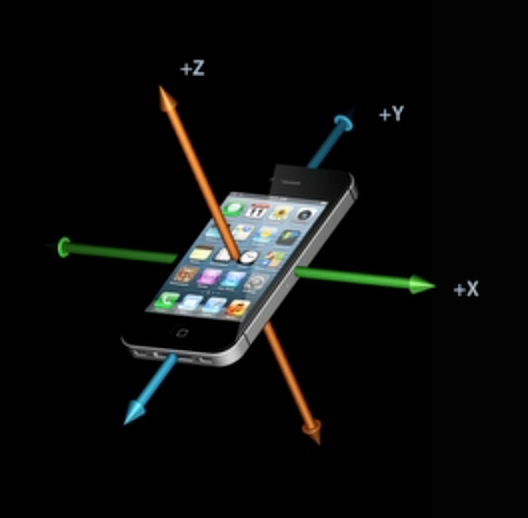
\includegraphics[width=0.4\textwidth]{figures/iphone_coordinatesystem}
	\caption{The iPhone's local coordinate system \citep{apple:wwdc_2012_pham}.}
	\label{fig:iphone_cs}
\end{figure}

\begin{figure}[p]
    \subfloat[XArbitrary]{
  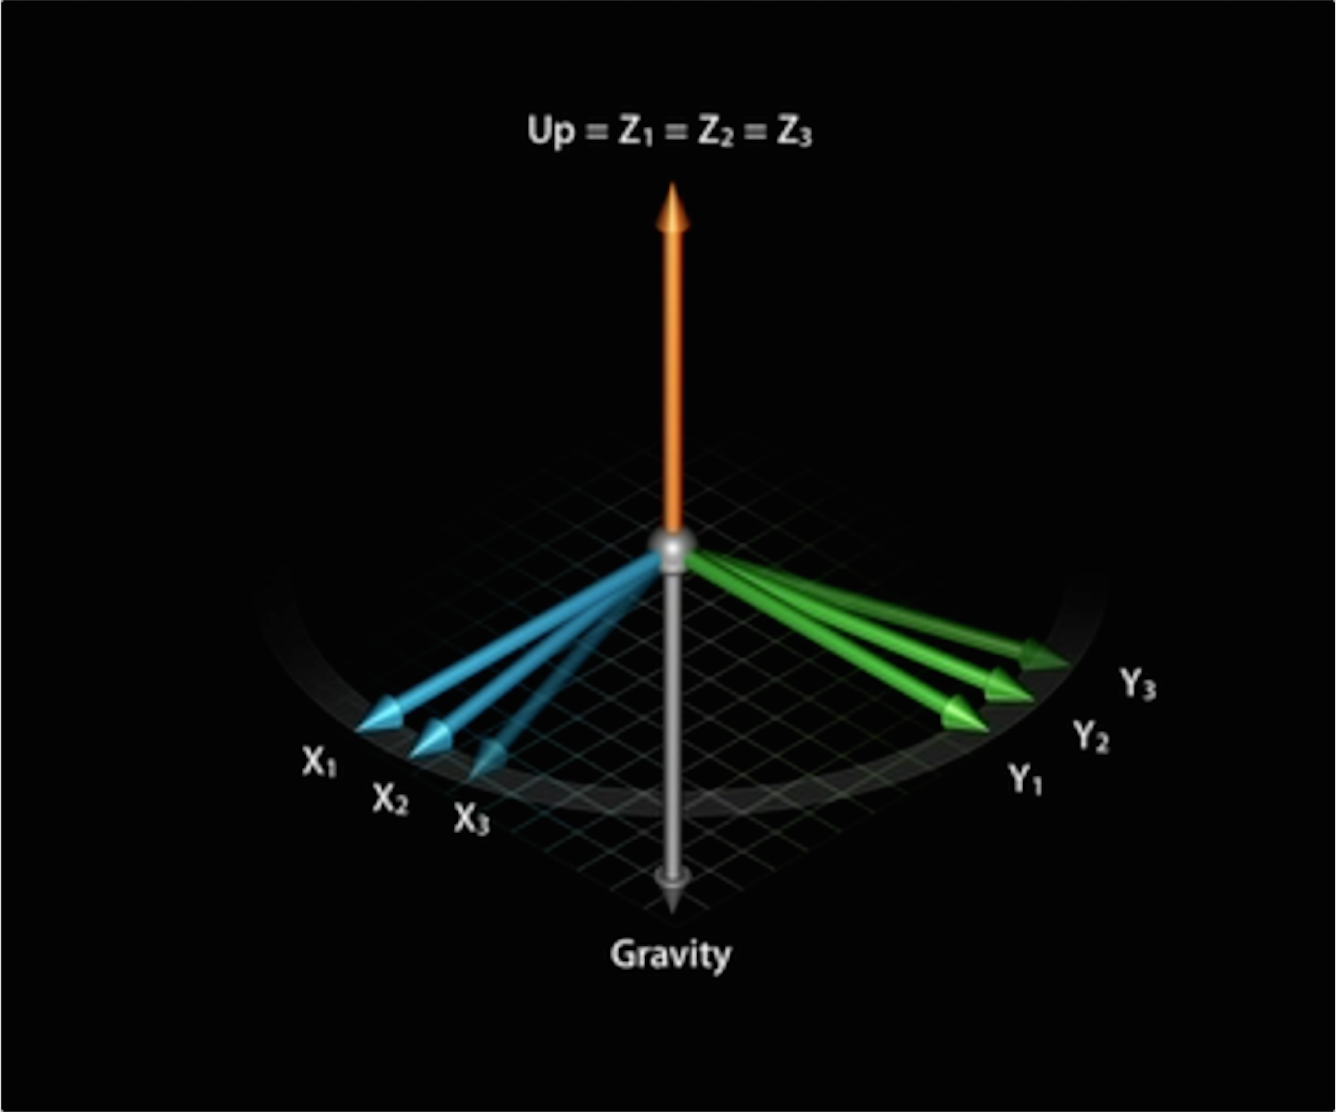
\includegraphics[width=0.4\textwidth]{figures/cm_xArbitrary}
  \label{fig:cm_referenceframes_xArbitrary}
}
\quad
\subfloat[XArbitraryCorrected]{
  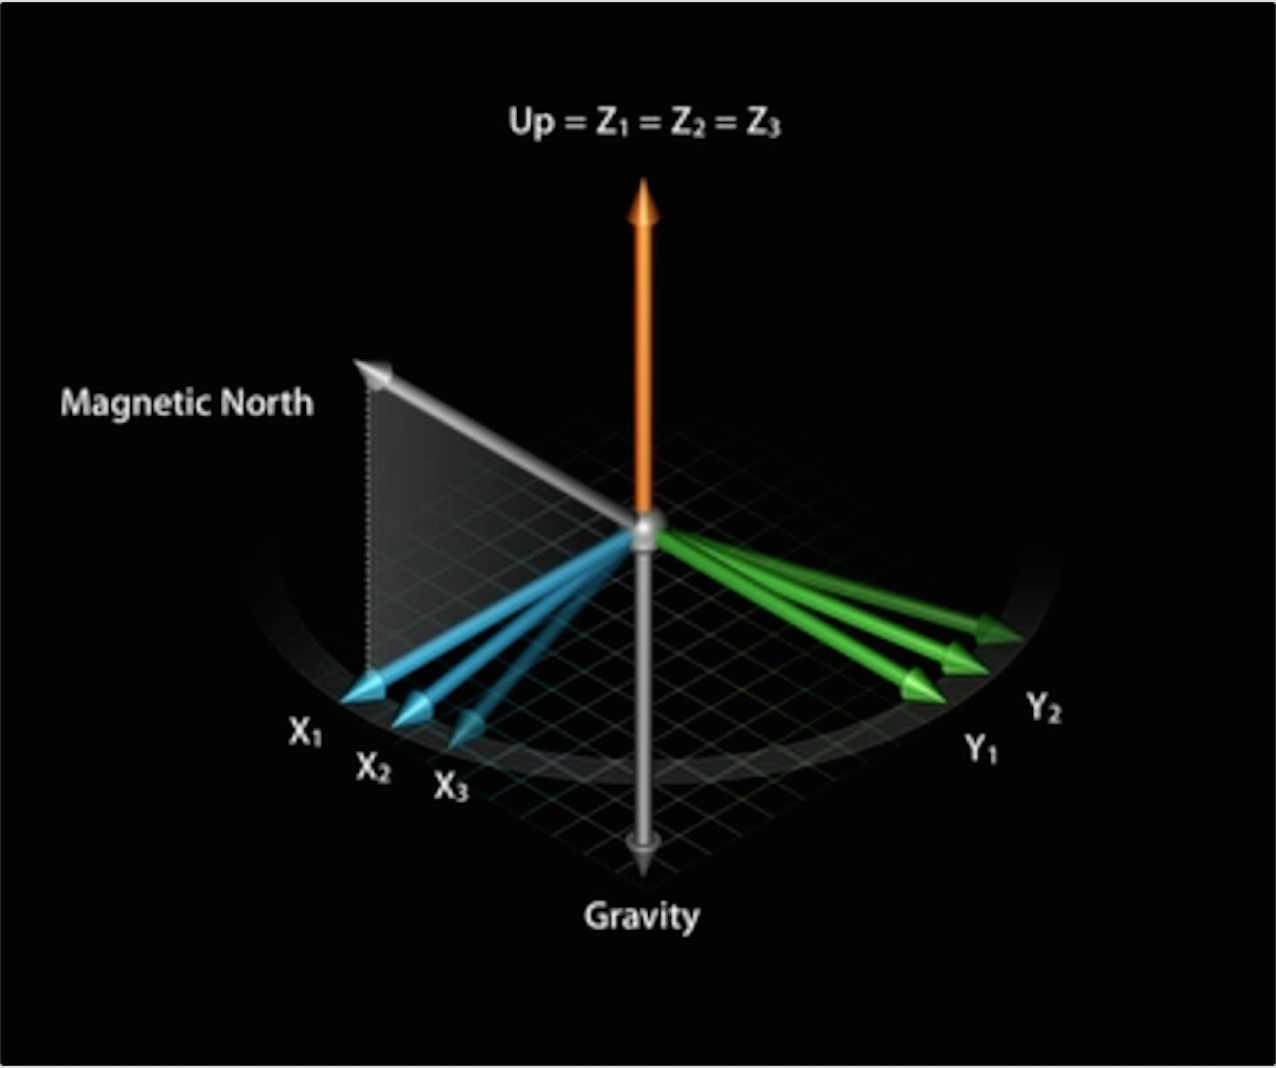
\includegraphics[width=0.4\textwidth]{figures/cm_xArbitraryCorrected}
  \label{fig:cm_referenceframes_xArbitraryCorrected}
}
\vspace{1cm}
\subfloat[XMagneticNorth]{
  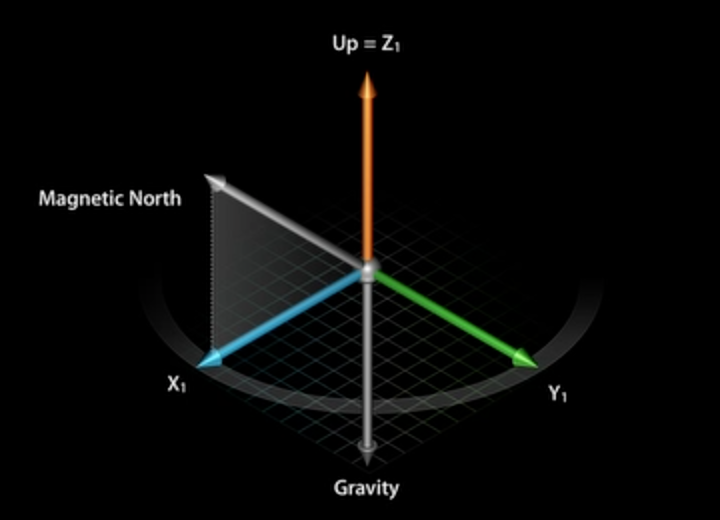
\includegraphics[width=0.4\textwidth]{figures/cm_xMagneticNorth}
  \label{fig:cm_referenceframes_xMagneticNorth}
}
\quad
\subfloat[XTrueNorth]{
  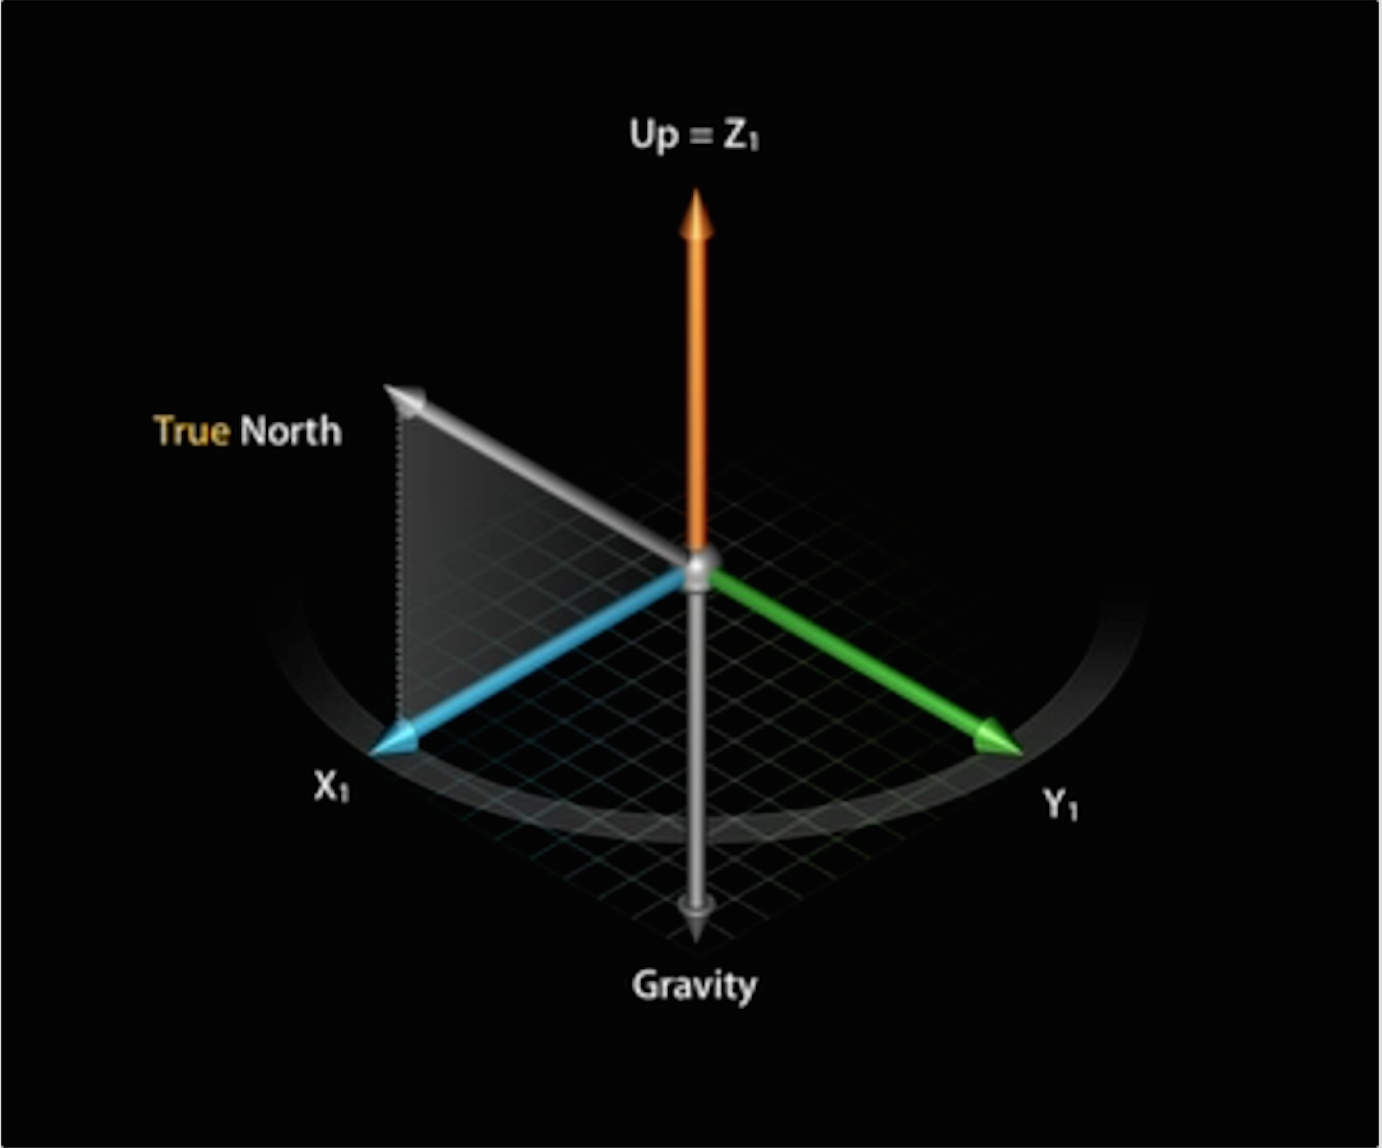
\includegraphics[width=0.4\textwidth]{figures/cm_xTrueNorth}
  \label{fig:cm_referenceframes_xTrueNorth}
}
  
	\caption{The \acl{CM} framework's attitude reference frames \citep{apple:wwdc_2012_pham}.}
	\label{fig:cm_referenceframes}
\end{figure}


As mentioned before, the iPhone contains a magnetometer, which is good for heading, an accelerometer, which can be used to calculate the phones tip and tilt, and a gyroscope to measure a device's rotation rate. To calculate the device's attitude, its position in three-dimensional space by using raw sensor data is very difficult, among things like uncertainty and ambiguity. Fortunately, Apple's \ac{CM} framework does not only provide raw sensor data, it also provides computed data like the \texttt{userAcceleration} and the device's \texttt{attitude} stored in their \texttt{CMDeviceMotion} component. To calculate these values, a technique, called \emph{sensor fusion}, is used. It combines the measurements of the before mentioned sensors, to reduce bias and uncertainties, and to remove ambiguities. Besides the \texttt{attitude}, the component also provides other data, such as:
\begin{itemize}
  \item \textbf{gravity}, in complete unconstraint motion
  \item \textbf{user acceleration} is the acceleration without gravity
  \item \textbf{rotation rate}, with compensated bias
  \item \textbf{magnetic field}, with removed disturbances
\end{itemize}

\noindent The mentioned values are all by-products of the device's attitude calculation \citep{apple:wwdc_2012_pham,apple:ios_doc_cm}.

\paragraph{Attitude} The device's attitude is provided in three different mathematical forms, Euler angles, Quaternions, and as rotation matrix.

To start receiving the device's \texttt{attitude} via the \texttt{CMDeviceMotionManager}, a reference frame needs to be specified. Figure~\ref{fig:iphone_cs} shows the iPhones local coordinate system, which is important to know, to understand the differences between the four possible reference frames. The four \texttt{CMAttitudeReferenceFrame}s, illustrated in Figure~\ref{fig:cm_referenceframes} have the vertical z-axis aligned with the gravity in common. According to \citet{apple:wwdc_2012_pham}, the specified reference frame also specifies the type of sensor fusion. The following reference frames exist \citep{apple:wwdc_2012_pham,apple:ios_doc_cm}:
\begin{itemize}
  \item \textbf{XArbitrary} (Figure~\ref{fig:cm_referenceframes_xArbitrary}): The x- and y-axis are unspecified. The initial position fixes the x and y orientation. There is no correction of the heading; it drifts over time.
  \item \textbf{XArbitraryCorrected} (Figure~\ref{fig:cm_referenceframes_xArbitraryCorrected}): The x- and y-axis are unspecified. The initial pose fixes the x- and y-orientation. Additionally, the magnetometer is used to correct heading and to improve yaw accuracy over time.
  \item \textbf{XMagneticNorth} (Figure~\ref{fig:cm_referenceframes_xMagneticNorth}): The x-axis is absolutely tagged to magnetic north. It uses the compass for orientation.
  \item \textbf{xTrueNorth} (Figure~\ref{fig:cm_referenceframes_xTrueNorth}): The x-axis is absolutely tagged to true north\footnote{The earth's magnetic field moves. Thus, true and magnetic north are not the same. Maps are oriented towards true north.}. It uses the compass to determine true north.
\end{itemize}



\subsection{Compass}
The compass is part of the \ac{CL} framework. It provides the device's \emph{magnetic heading} and also its \emph{true heading} in degrees. The heading depends on the specified device orientation, such as portrait, landscape left, or landscape right mode \citep{apple:ios_doc_cl}. According to \citet{apple:wwdc_2012_pham}, the compass uses sensor fusion and not only the magnetometer.

To access the device's heading, the \texttt{CLLocationManager} must be configured. It informs the application when the heading changes. The developer can specify a heading filter. Thus, a new heading is only reported, if the heading filter is exceeded \citep{apple:ios_doc_cl}.

As already mentioned before, the magnetometer measures the magnetic field, which is not only the earth's magnetic field. It is biased; for example, by iron bars and AC current. To reduce bias, the compass asks the user to calibrate it, by moving the device in a specific manner. \ac{CL} by itself can detect whether or not the compass needs calibration. Thus, it automatically shows the user the calibration view \citep{apple:ios_doc_cl}.


\section{Evaluation}\label{sec:sensor_eval}
The purpose of this section is to find out if the above referenced sensors and \acsp{API} are suitable for this project. In the following the provided data is evaluated. Furthermore, the above referenced statements made by Apple's engineers are verified.


\subsection{MotionActivity}
As mentioned above, the purpose of the \texttt{CMMotionActivity} component is to detect and classify a user's activity. To prove the statement concerning the recognition duration of the walking state made by Apple's engineer \citet{apple:wwdc_2014_pham} some test walks were performed. The results of the experiment show, that the claim of a recognition time of 10\,--\,15\,s for the walking state is very optimistic. Table~\ref{tab:motionActivityEvaluation} shows the beginning of one of these test walks.

From the start, the test user walked with constant speed and with the phone in hand. It shows that the component recognize when the device was moving (not stationary) even before the application started (Table~\ref{tab:motionActivityEvaluation}, Line 1). In reality, the application was started before starting to walk, but \emph{not stationary} means that the user just somehow moves the device. After $\approx$\,10.7\,s the component increases its confidence for the current state (Table~\ref{tab:motionActivityEvaluation}, Line 2). Another $\approx$\,5\,s later it set the confidence to \texttt{high} (Table~\ref{tab:motionActivityEvaluation}, Line 3); thus, the component is very confident that the user somehow moves the device. After $\approx$\,25\,s of walking the component finally detects with \texttt{low} confidence, that the user actually walks (Table~\ref{tab:motionActivityEvaluation}, Line 4).

Compared to detecting the users walking state, it detects nearly in real-time, that the user stops walking after $\approx$\,32\, (Table~\ref{tab:motionActivityEvaluation}, Line 5). At this point in time the user holds the device very steady. The component only switches between stationary and not stationary, in a very short time period (Table~\ref{tab:motionActivityEvaluation}, Line 5\,--\,7).

This experiment shows that the user needs to actually walk a very long distance until the phone recognizes that the user is walking. It also shows that the user has to hold the device very steady until the device claims that the device is stationary. Consequently, \ac{CM}'s \texttt{CMMotionActivity} cannot really be used to determine a user's walking state for short distances. Also the stationary state cannot be used to claim that the user is not walking due to the high sensibility.

\begin{table}
	\begin{tabular}{l*{7}{c}}
start date & confidence & unknown & stationary & walking & running & automotive & cycling \\
\hline
-2.0246 & 0 & false & false & false & false & false & false\\
10.7026 & 1 & false & false & false & false & false & false\\
15.7922 & 2 & false & false & false & false & false & false\\
25.9676 & 0 & false & false & \textbf{true} & false & false & false\\
32.3255 & 1 & false & \textbf{true} & false & false & false & false\\
32.6434 & 1 & false & false & false & false & false & false\\
33.2792 & 1 & false & \textbf{true} & false & false & false & false\\
\dots & \dots & \dots & \dots & \dots & \dots & \dots & \dots
\end{tabular}

	\caption{Recorded \texttt{CMMotionActivity} data during a test walk. The user stopped at $\approx$\,32\,s. Remark: To simplify the table the start date is shown as relative timestamp instead of an absolute date.}
	\label{tab:motionActivityEvaluation}
\end{table}


\subsection{Pedometer}
To evaluate the accuracy of \ac{CM}'s \texttt{CMPedometer} component, test walks of different distances  were performed, to compare the actual distance and step count with the measured values. Due to the fact that users usually carry their smartphone in their trouser pockets or hold it in their hand, the experiment was performed for both positions. Figure~\ref{fig:eval:pedometerHand} shows the measured distances and the corresponding step counts for different distances with the phone in hand. The results of the same experiment with the phone in the trouser pocket are shown in Figure~\ref{fig:eval:pedometerPocket}.

The experiments visualization shows the measurements dispersion. Sometimes, the \texttt{CMPedometer} overestimates or underestimates the distance, i.e.\ the step count. The experiment also shows, that the phone on average underestimates the values, if the user holds the device in hand. If the user walks with the phone in the trouser pocket the device also underestimates the measured distances; whereas, the measured step counts are more precise.

Figure~\ref{fig:eval:pedometerNDF} depicts the \texttt{CMPedometer}'s standard deviation $\sigma$ depending on the distance and phone's position. To model the uncertainty for any walked distance, depending on the smartphone's position, linear regression based on the measurements was used. Initially, I expected a higher accuracy of the estimated distance if the user carries the phone in the trouser pocket, but the diagram prooves the opposite. Consequently, $\sigma$ is significantly smaller if the user holds the phone in hand.

% CMPedometer (step count, distance)  dispersion plots
\begin{figure}[p]
    \subfloat[Estimated Distances]{
  \begin{tikzpicture}
  \begin{axis}[width=0.45\textwidth, height=0.4\textheight,
    xlabel={Reference Distance (m)},
    ylabel={Estimated Distance (m)},
    legend entries={measurement, average},
    legend pos=south east,
    grid = major]
    \addplot [blue, only marks, mark=x] table[col sep=semicolon, x=distanceRef, y=distance] {csv/2014-10-28_htwg_keller_f/inHand.csv};
    \addplot [blue, only marks, mark=triangle*, mark size=3pt] table[col sep=semicolon, x=distanceRef, y=distance] {csv/2014-10-28_htwg_keller_f/inHand_avg.csv};
  \end{axis}
  \end{tikzpicture}
  \label{fig:eval:pedometerHand:dist}
}
\quad
\subfloat[Estimated Step Count]{
  \begin{tikzpicture}
  \begin{axis}[width=0.45\textwidth, height=0.4\textheight,
    xlabel={Reference Distance (m)},
    ylabel={Estimated Step Count},
    legend entries={measurement, average, ref. step count},
    legend pos=south east,
    grid = major]
    \addplot [blue, only marks, mark=x] table[col sep=semicolon, x=distanceRef, y=steps] {csv/2014-10-28_htwg_keller_f/inHand.csv};
    \addplot [blue, only marks, mark=triangle*, mark size=3pt] table[col sep=semicolon, x=distanceRef, y=steps] {csv/2014-10-28_htwg_keller_f/inHand_avg.csv};
    \addplot [green, only marks, mark=*, mark size=3pt] table[col sep=semicolon, x=distanceRef, y=stepRef] {csv/2014-10-28_htwg_keller_f/inHand_avg.csv};
  \end{axis}
  \end{tikzpicture}
  \label{fig:eval:pedometerHand:steps}
}
  
	\caption{Measured distances and step counts for different reference distances estimated by \ac{CM}'s \texttt{CMPedometer}. The measurements were taken indoor on a hard floor with the smartphone in hand.}
	\label{fig:eval:pedometerHand}
\end{figure}

\begin{figure}[p]
  \subfloat[Measured Distances]{
  \begin{tikzpicture}
  \begin{axis}[width=0.45\textwidth, height=0.4\textheight,
    xlabel={Reference Distance (m)},
    ylabel={Estimated Distance (m)},
    legend entries={measurement, average},
    legend pos=south east,
    grid = major]
      \addplot [red, only marks, mark=x] table[col sep=semicolon, x=distanceRef, y=distance] {csv/2014-10-28_htwg_keller_f/inPocket.csv};
  \addplot [red, only marks, mark=triangle*, mark size=3pt] table[col sep=semicolon, x=distanceRef, y=distance] {csv/2014-10-28_htwg_keller_f/inPocket_avg.csv};
  \end{axis}
  \end{tikzpicture}
  \label{fig:eval:pedometerPocket:dist}
}
\quad
\subfloat[Measured Step Count]{
  \begin{tikzpicture}
  \begin{axis}[width=0.45\textwidth, height=0.4\textheight,
    xlabel={Reference distance (m)},
    ylabel={Estimated Step Count},
    legend entries={measurement, average, ref.\ step count},
    legend pos=south east,
    grid = major]
      \addplot [red, only marks, mark=x] table[col sep=semicolon, x=distanceRef, y=steps] {csv/2014-10-28_htwg_keller_f/inPocket.csv};
  \addplot [red, only marks, mark=triangle*, mark size=3pt] table[col sep=semicolon, x=distanceRef, y=steps] {csv/2014-10-28_htwg_keller_f/inPocket_avg.csv};
  \addplot [green, only marks, mark=*, mark size=2pt] table[col sep=semicolon, x=distanceRef, y=stepRef] {csv/2014-10-28_htwg_keller_f/inPocket_avg.csv};
  \end{axis}
  \end{tikzpicture}
  \label{fig:eval:pedometerPocket:steps}
}

  \caption{Measured distances and step counts for different reference distances estimated by \ac{CM}'s \texttt{CMPedometer}. The measurements were taken indoor on a hard floor with the smartphone in trouser pocket.}
  \label{fig:eval:pedometerPocket}
\end{figure}

Besides the pedometer's accuracy also the duration until the component detects that the user is walking and thus delivers the first distance estimation was evaluated. The \texttt{CMPedometer} component on average needs 5\,--\,10\,s to deliver the first estimation, which is also consistent with a statement made by \citet{apple:wwdc_2014_pham}. The first estimation typically contains a step count of 6\,--\,8. Once it detects that the user is walking, it continuously delivers updates every $\approx$\,2.5\,s.

Another interesting value is the time it takes the pedometer to recognize that the user continues walking after a short break of $\approx$\,10\,--\,15\,s. Against my expectation, it takes approximately the same amount of time and also the same amount of steps as the component requires to recognize it the first time. This behavior is depicted in Table~\ref{tab:pedometerEvaluation}. First it shows the amount of time and steps it took the component to recognize that the user is walking (Table~\ref{tab:pedometerEvaluation}, Line 1). After 50\,steps the user took a short break of around 15\,s (Table~\ref{tab:pedometerEvaluation}, Line 5). Furthermore it shows that the component requires 6\,steps to recognize that the user continued walking (Table~\ref{tab:pedometerEvaluation}, Line 7). The third data block shows another break that the user made during the test walk (Table~\ref{tab:pedometerEvaluation}, Line 9\,--\,11).

\begin{figure}
  \begin{tikzpicture}
    \begin{axis}[trim axis left, trim axis right, width=0.9\textwidth, height=0.4\textheight,
        xlabel={Distance / Mean $\mu$ (m)},
        ylabel={Standard deviation $\sigma$ (m)},
        legend entries={in hand, $f(\mu)=0.0971 \cdot \mu + 1.445$, in pocket, $f(\mu)=0.1971 \cdot \mu + 2.8703$},
        legend pos=north west,
      grid = major]
      \addplot [blue, mark=*] table[col sep=semicolon, x=mu_distanceRef, y=sigma_distanceRef] {csv/2014-10-28_htwg_keller_f/inHand_ndf_parameters.csv};
      %      \addplot [blue, dashed, domain=0:30, samples=2]{0.0680*x+2.1559};
      \addplot [blue, dashed, domain=0:30, samples=2]{0.0971*x+1.445};
      \addplot [red, mark=*] table[col sep=semicolon, x=mu_distanceRef, y=sigma_distanceRef] {csv/2014-10-28_htwg_keller_f/inPocket_ndf_parameters.csv};
      \addplot [red, dashed, domain=0:30, samples=2]{0.1971*x+2.8703};
    \end{axis}
\end{tikzpicture}

  \caption {The \texttt{CMPedometer} component's uncertainty and their approximation using linear regression depending on the walked distance and the phone's position.}
  \label{fig:eval:pedometerNDF}
\end{figure}

\begin{table}
	\begin{tabular}{*{4}{l}}
startDate & endDate & distance & steps\\
\hline
0.0019 & 8.2329 & 4.8273 & 7\\
0.0019 & 10.7811 & 7.9850 & 11\\
0.0019 & 13.3238 & 11.4785 & 16\\
\dots & \dots & \dots & \dots\\
0.0019 & 31.1349 & 37.2110 & 50\\
0.0019 & 54.0149 & 37.2110 & 50\\
0.0019 & 56.5503 & 41.4032 & 56\\
\dots & \dots & \dots & \dots\\
0.0019 & 69.2608 & 57.2046 & 78\\
0.0019 & 84.5138 & 57.2046 & 78\\
0.0019 & 87.0569 & 64.8046 & 88
\end{tabular}

	\caption{Recorded \texttt{CMPedometer} example data. Remark: To simplify the table relative timestamps for startDate and endDate are used. All values except the steps are truncated.}
	\label{tab:pedometerEvaluation}
\end{table}


\subsection{Heading}
As mentioned earlier, the solution's localization algorithm, introduced in Chapter~\ref{chap:pf}, needs heading for the motion tracking to determine in which direction the user is moving. To get the devices' heading, either the \texttt{CMAttitude} provided by \ac{CM}, or the \texttt{CLHeading} provided by \ac{CL} can be used. In this section first the \texttt{CMAttitude}'s data is evaluated and afterwards the data provided by \texttt{CLHeading}.

\subsubsection*{CMAttitude}
As mentioned before, the \texttt{CMAttitude} data is provided as Euler angles, Quaternions and as rotation matrix. To be able to compare attitude with compass heading, it is of advantage to transform the attitude into a heading in compass degrees. This means, if the device top is pointing towards magnetic north, the heading $\theta = 0^{\circ}$, east $\theta = 90^{\circ}$, south $\theta = 180^{\circ}$, and west $\theta = 270^{\circ}$. Equation\,\ref{eq:rotationmatrix} shows the 3-dimensional rotation matrix provided by \texttt{CMAttitude} as specified in the \ac{CM}'s documentation \citep{apple:ios_doc_cm}. The calculation of $\theta$ in compass degrees, where $m_{1,2}$ and $m_{2,2}$ describe the transformation of the phone's y-axis by the rotation around its z-axis, is shown in Equation\,\ref{eq:rotation2heading}.

\begin{equation} \label{eq:rotationmatrix}
  M_{3,3} = \begin{pmatrix}
      m_{1,1} & m_{1,2} & m_{1,3} \\
      m_{2,1} & m_{2,2} & m_{2,3} \\
      m_{3,1} & m_{3,2} & m_{3,3}
  \end{pmatrix}
\end{equation}

\begin{equation} \label{eq:rotation2heading}
  \theta = (\pi + {\rm atan2}\left(m_{2,2} , m_{1,2}\right)) \cdot \frac{180.0}{\pi}, \quad \text{for } m_{2,2}, m_{1,2} \neq 0
\end{equation}

\noindent As mentioned earlier, the \texttt{CMAttitude}'s values depend on the specified reference frame, which also affects the sensor fusion algorithm. To be able to easily compare the calculated heading $\theta$ directly with the compass heading the \texttt{xMagneticNorth} reference frame is used. Thus, z is aligned to gravity and x points towards magnetic north.

\begin{figure}
	\subfloat[\texttt{xMagneticNorth} Reference Frame]{
		\begin{tikzpicture}
\begin{axis}[width=0.5\textwidth, height=0.4\textheight,
  xlabel={round},
  ylabel={heading error (degree)},
  legend entries={counter-clockwise, clockwise},
  legend pos=north west,
  grid = major]
  \addplot [blue, mark=*] table[col sep=semicolon, x=round, y=error_attitude] {csv/deviceAttitudeAndCompass/xMagneticNorthAndCompass_left.csv};
\addplot [blue, dashed, mark=*] table[col sep=semicolon, x=round, y=error_attitude] {csv/deviceAttitudeAndCompass/xMagneticNorthAndCompass_right.csv};
\end{axis}
\end{tikzpicture}

		\label{fig:evalAttitude:xMagneticNorth}
	}
	\subfloat[Different Reference Frames]{
		\begin{tikzpicture}
\begin{axis}[width=0.5\textwidth, height=0.4\textheight,
  xlabel={Rounds},
  ylabel={Heading Error (degree)},
  legend entries={xMagneticNorth, xArbitrary, xArbitraryCorrected},
  legend pos=north west,
  grid = major]
  \addplot [blue, mark=*] table[col sep=semicolon, x=round, y=error_attitude] {csv/deviceAttitudeAndCompass/xMagneticNorthAndCompass_left.csv};
\addplot [red, mark=*] table[col sep=semicolon, x=round, y=error_attitude] {csv/deviceAttitudeAndCompass/xArbitraryAndCompass.csv};
\addplot [green, mark=*] table[col sep=semicolon, x=round, y=error_attitude] {csv/deviceAttitudeAndCompass/xArbitraryCorrectedAndCompass.csv};
\end{axis}
\end{tikzpicture}

		\label{fig:evalAttitude:referenceframes}
	}
	
	\caption{Depicts the \texttt{CMAttitude}'s heading drift using the \texttt{xMagneticNorth} reference frame in clockwise and counter-clockwise direction. Furthermore, it compares the heading drift in counter-clockwise direction using different reference frames. To evaluate this a test person walked 10 times around a small table in clockwise and counter-clockwise direction.}
\end{figure}

%\begin{figure}[p]
%	\begin{tikzpicture}
\begin{axis}[width=0.5\textwidth, height=0.4\textheight,
  xlabel={Rounds},
  ylabel={Heading Error (degree)},
  legend entries={xMagneticNorth, xArbitrary, xArbitraryCorrected},
  legend pos=north west,
  grid = major]
  \addplot [blue, mark=*] table[col sep=semicolon, x=round, y=error_attitude] {csv/deviceAttitudeAndCompass/xMagneticNorthAndCompass_left.csv};
\addplot [red, mark=*] table[col sep=semicolon, x=round, y=error_attitude] {csv/deviceAttitudeAndCompass/xArbitraryAndCompass.csv};
\addplot [green, mark=*] table[col sep=semicolon, x=round, y=error_attitude] {csv/deviceAttitudeAndCompass/xArbitraryCorrectedAndCompass.csv};
\end{axis}
\end{tikzpicture}

%	\caption{Compares \texttt{CMAttitude}'s heading drift using different reference frames. The test person walked 10 times around a small table in counter-clockwise direction.}
%	\label{fig:evalAttitude:referenceframes}
%\end{figure}

The most important requirement for heading is long-term accuracy. To test this, the test person walked 10\,times around a small table in the same direction and recorded the heading after each round. To record the heading after each round the device was put on the table at the exact same position. Thus, the heading should be roughly the same after each round. Figure~\ref{fig:evalAttitude:xMagneticNorth} illustrates the error of each measurement compared to the initial measurement. First, the test person walked counter-clockwise around the table. An enormous drift of $\approx 30^{\circ}$ after each round was observed. This sums up to a total drift of $\approx 300^{\circ}$ after 10 rounds. To confirm this, the person walked also clockwise around the table and observed the same amount of drift in the opposite direction. Apple's engineer, \citet{apple:wwdc_2012_pham}, explicitly mentioned that the magnetometer is used to provide long-term yaw accuracy, if the \texttt{xArbitraryCorrected} reference frame is specified. Thus, the same test was repeated for the \texttt{xArbitrary} and the \texttt{xArbitraryCorrected} reference frame. Then the results were compared with the results from before, shown in Figure~\ref{fig:evalAttitude:referenceframes}. There is nearly no difference in long-term accuracy between the three tested reference frames.

\subsubsection*{CLHeading}
During the before mentioned experiment, shown in Figure~\ref{fig:evalAttitude:xMagneticNorth} and \ref{fig:evalAttitude:referenceframes}, the compass, i.e.\ \texttt{CLHeading}, values were recorded as well. Figure~\ref{fig:eval:compass} shows the heading's error over time. The chart shows no drift over time compared to the data measured by \texttt{CMAttitude}. However, it also shows that the compass can be biased by other magnetic fields. The outliers in the experiment with counter-clockwise direction led me to assume that another magnetic field biased the before measured magnetic field.

That the compass reacts on other magnetic fields, than the earth's magnetic field can easily be shown by moving a small magnet around the phone. In contrast to the compass, the \texttt{CMAttitude} does not react to other magnetic fields, like the one of a magnet.

According to the 40\,measurements depicted in Figure~\ref{fig:eval:compass}, the compass's standard deviation $\sigma$ amounts to $3.1^{\circ}$. During the experiment the \texttt{CLHeading} components heading filter was set to $1.0^{\circ}$.


\begin{figure}
	\begin{tikzpicture}
\begin{axis}[width=0.6\textwidth, height=0.4\textheight,
  xlabel={round},
  ylabel={heading error (degree)},
  grid = major]
  \addplot [blue, mark=*] table[col sep=semicolon, x=round, y=error_compass] {csv/deviceAttitudeAndCompass/xMagneticNorthAndCompass_left.csv};
\addplot [blue, dashed, mark=*] table[col sep=semicolon, x=round, y=error_compass] {csv/deviceAttitudeAndCompass/xMagneticNorthAndCompass_right.csv};
\addplot [red, mark=*] table[col sep=semicolon, x=round, y=error_compass] {csv/deviceAttitudeAndCompass/xArbitraryAndCompass.csv};
\addplot [green, mark=*] table[col sep=semicolon, x=round, y=error_compass] {csv/deviceAttitudeAndCompass/xArbitraryCorrectedAndCompass.csv};
\end{axis}
\end{tikzpicture}

	\caption{\texttt{CLHeading}'s, i.e.\ the compass' magnetic heading's drift. The test person walked 10 times around a small table in clockwise and counter-clockwise direction. The initial measurement is used as reference value. The heading filter was set to $1.0^{\circ}$. The measurements (lines colors) belong to the ones presented in Figure~\ref{fig:evalAttitude:xMagneticNorth} and \ref{fig:evalAttitude:referenceframes}.}
	\label{fig:eval:compass}
\end{figure}

\subsection{Summary}
As advertised, the solution explained in Chapter~\ref{chap:pf}, is based on \ac{MCL}. Thus, motion tracking is required, which seems to be feasible by combining \ac{CM}'s distance estimation and \ac{CL} heading. If the \texttt{CLHeading} is heavily influenced by other materials, like iron bars, it could probably be reasonable to also integrate the discussed heading based on \ac{CM}'s attitude. But, due to its huge drift problem, only the change in heading, i.e.\ the rotation rate, can be used.

Furthermore, \ac{CM}'s motion activity classification seems to be useless for the later presented solution due to its huge latency.

\chapter{Localization Algorithm} \label{chap:pf}
This chapter presents the solution's implementation. As mentioned before, it is based on \acf{MCL}. The terminology used in this chapter builds upon the \acs{PF}'s introduction in section~\ref{sec:fund_pf}.

First the reasons for choosing \acs{MCL} instead of another algorithm are outlined. Afterwards, an overview of the system's setup is provided. Next the algorithm's \emph{motion model} is described, followed by a detailed insight in the solution's \emph{measurement model}. In the end, the algorithm's implementation is described, which builds upon the motion and measurement model.


\section{Design Decision} \label{sec:algo_decision}
This section outlines the reasons for choosing \acl{MCL} instead of another algorithm, as introduced in chapter~\ref{chap:fundamentals}.

As shown in chapter~\ref{chap:ibeacons} and mentioned by \citet{IEEE:survey_wireless_indoor_pos}, wireless signals are heavily influenced by obstacles and their environment. According to \citet{wang:wlan} and \citet{siddiqi:experiments_mcl_wifi}, location accuracy can be drastically improved by additionally using map information and motion tracking. Thus, the main reason for choosing \ac{MCL} is the fact, that \acl{PF} is the only algorithm, which has the ability to combine the \acs{RSS}-based measurements to the beacons with motion tracking by additionally using map information. Triangulation, the proximity method, and the scene analysis approach are not able to improve their location estimation by combining motion tracking with \ac{RSS}-based measurements. \acl{KF} is the only algorithm which is also capable of using motion besides \ac{PF}. But according to \citet{wang:wlan}, ``map information is impossible to be integrated for tracking by \acs{EKF}''.

The second reason for choosing \acs{PF} is its ability to solve the \emph{global localization problem}. Thus, the algorithm can start determining the user's location without knowing the user's initial position. Furthermore, the algorithm is able to recover form failure state, i.e.\ if the estimated location is completely wrong, e.g. due to short-term sensor failure, it is able to detect and to recover from that state.

The third reason is the algorithm's advantage of taking uncertainties into account. Besides \ac{PF}, \ac{KF} is the only mentioned algorithm which is also capable of modeling uncertainties. As mentioned before, \acs{PF} is a non-parametric filter with the advantage of expressing a location estimation in the form of a multi-modal posterior belief. Whereas \ac{KF} is a parametric filter which is fixed to normal distributed position estimations. Furthermore, the \ac{PF}'s multi-modal belief can be visually illustrated very well and the users can benefit from this as shown in figure~\ref{fig:pf_approx}.

The fourth reason are the, in chapter~\ref{chap:intro} defined, requirements. By using \acs{PF}, based on \acs{RSS}-based measurements, less pre-deployment effort is required. Furthermore, the required infrastructure is of little complexity compared to other solutions outlined in chapter~\ref{chap:fundamentals}, which reduces the maintenance effort and the initial and maintenance costs.

Besides the above mentioned reasons, \acl{PF} is an easy-to-implement algorithm. Furthermore, \ac{MCL} is a well-known and well-studied approach for landmark-based localization in robotics, as mentioned by \citet{thrun:prob_robo}.


\section{System Setup}
Before going into the detailed description of the solution, this section provides an overview of the system setup.

The implementation is written in Apple's new programming language \emph{Swift} (version 1.2), which is the successor of \emph{Objective-C}. The language is based on modern programming concepts, such as functional programming, tuples, generics, etc. Furthermore, Apple tries to remove unsafe code, such as not initialized variables, null-pointers, array overflows, etc.\ by defining the language's elements in a very concise and expressive syntax, and by adding new language constructs and types, such as the Optional type. The language compiles to native code by using LLVM compiler. Swift code can also call C and Objective-C code, which provides the possibility to use Swift in existing projects \citep{apple:swift}.

\begin{figure}[height=0.45\textheight]
	\begin{tikzpicture}
 %\draw[style=help lines] (0,0) grid (15,10);

 % sensors
 \node (A) at (13,9) {Accelerometer};
 \node (G) at (13,7) {Gyroscope};
 \node (M) at (13,5) {Magnetometer};
 \node (B) at (13,2) {\acs{BLE}};

 \draw (A) ellipse (1.5 and 0.5);
 \draw (G) ellipse (1.5 and 0.5);
 \draw (M) ellipse (1.5 and 0.5);
 \draw (B) ellipse (1.5 and 0.5);

 % Frameworks
 \node (CMP) at (8,8) {\texttt{CMPedometer}};
 \node (CMDM) at (8,6) {\texttt{CMDeviceMotion}};
 \node (CLH) at (8,4) {\texttt{CLHeading}};
 \node (CLB) at (8,2) {\texttt{CLBeacon}};
 \node (MAP) at (8,0) {Map};

 \draw (6,7.5) rectangle (10,8.5);
 \draw (6,5.5) rectangle (10,6.5);
 \draw (6,3.5) rectangle (10,4.5);
 \draw (6,1.5) rectangle (10,2.5);
 \draw (6,-0.5) rectangle (10,0.5);


 \draw[very thick] (11.5,9) -- ++(-0.5,0) -- ++(0,-2) -- ++(0.5,0) -- ++(-0.5,0) -- ++(0,-1.9) -- ++(0.5,0);
 \draw[->, very thick] (11,8) to (10,8);
 \draw[->, very thick] (11,6) to (10,6);


 \draw[->, very thick] (11.5,4.9) -- ++(-0.5,0) -- ++(0,-0.9) -- ++(-1,0);
 \draw[->, very thick] (11.5,2) to (10,2);

 % Particle Filter
 \draw (-0.5,-1) rectangle (4.5,9);
 \node (MM) at (2,8.5) {\textbf{Particle Filter}};

 % Motion Model
 \draw (0,5) rectangle (4,7);
 \node (MM) at (2,6) {Motion Model};

 \draw[->, very thick] (6,8) to (4,6.2);
 \draw[->, very thick] (6,6) to (4,6);
 \draw[->, very thick] (6,4) to (4,5.8);

 % Measurement Model
 \draw (0,0) rectangle (4,2);
 \node (MM) at (2,1) {Measurement Model};

 \draw[->, very thick] (6,2) to (4,1.1);
 \draw[->, very thick] (6,0) to (4,0.9);

 % Location
 \node (L) at (2,-2.5) {$\chi$};
 \draw (L) ellipse (0.5 and 0.5);
 \draw[->, very thick] (2,-1) -- ++(0,-1);
 \draw[->, very thick] (1.5,-2.5) -- ++(-2.25,0) -- ++(0,12.5) -- ++(2.75,0) -- ++(0,-1);

\end{tikzpicture}

	\caption{Depicts the solution's setup}
	\label{fig:algo_architecture}
\end{figure}

The system, depicted in figure~\ref{fig:algo_architecture}, consists of the \ac{PF}, its components, and the used \acsp{API}. Furthermore, the figure depicts the sensors used by the \acsp{API}. As explained in section~\ref{sec:fund_pf}, the algorithm uses two models, the \emph{Motion Model} and the \emph{Measurement Model}.

The Motion Model, described in section~\ref{sec:algo_motion_model}, is on one hand, responsible for tracking the user's motion by combining different sources. On the other hand, it samples from the motion model. To implement this, the Core Motion framework's pedometer and device motion component are used, which both use the smartphone's accelerometer, gyroscope and magnetometer, as described in chapter~\ref{chap:sensors}. Furthermore, the component uses the Core Location framework's compass, i.e.\ \texttt{CLHeading}, which uses the magnetometers data.

The Measurement Model, described in section~\ref{sec:algo_measurement_model}, implements the \acs{PF}'s importance factor calculation. For that it uses Core Location's \texttt{CLBeacon} component, which provides the \acs{RSS}-based distances estimations to the beacons. It uses the smartphone's \acf{BLE} module, to receive the beacons' \ac{BLE} signals. Furthermore, the Measurement Model uses the building's map.

The \acl{PF}, described in section~\ref{sec:algo_pf}, outputs the posterior, i.e.\ the position estimation represented by the particle set $\chi$. Furthermore, $\chi$ is passed to the function by its next iterative call.


\section{Motion Model}\label{sec:algo_motion_model}
The solution's motion model component is responsible for three tasks, firstly, for tracking the users motion, secondly, to determine if the user is stationary, and thirdly, to allow the \acs{PF} to sample from the motion model. The three tasks are prerequisites for the later explained \acs{PF} implementation.

\subsection{Motion Tracking}
As mentioned in chapter~\ref{chap:sensors}, \acl{CM} provides a component called \texttt{CMPedometer}, which estimates the traveled distance based on the steps a user has taken. In addition, \acl{CL} provides the smartphone's heading, based on the magnetic field, called \texttt{CLHeading}. Furthermore, \ac{CM}'s \texttt{CMDeviceMotion} provides the device attitude, which is calculated by using sensor fusion. The device's attitude can also be used to calculate the device's heading. By combining these three sources, the user's motion can be tracked, and a path can be constructed.

\subsubsection*{Heading}
As mentioned in chapter~\ref{chap:sensors}, the heading provided by \texttt{CLHeading} can be influenced by other magnetic fields than the earth's magnetic field, which may cause wrong values. \texttt{CMDeviceMotion} uses sensor fusion instead of relying only on the magnetometer's values. Thus, it is not influenced by other magnetic fields, but against the claims made by Apple's engineer \citet{apple:wwdc_2012_pham}, the values tend to drift away. Consequently, only relying on \texttt{CMDeviceMotion} is not sufficient. As a result, both sources are combined to determine the smartphone's heading.

Both frameworks do provide their values asynchronously. \acs{CL} calls its delegate method if a certain threshold of the heading's change, set to $1^\circ$, exceeds. Whereas, \acs{CM} calls its delegate periodically, every 0.02s. The high update rate would not be necessary for heading, but as mentioned earlier \texttt{CMDeviceMotion} also includes \texttt{userAccleration}, which is used for the stationary detection, as shown later.

The \texttt{CMDeviceMotion} heading, further denoted as $\theta_A$, measured at time $t$, is calculated from the rotation matrix, given by \texttt{CMDeviceMotion.attitude}, as explained in chapter~\ref{chap:sensors}. Due to its drift problem only the change between two values, denoted as $\Delta\theta_A$ is used. For the absolute orientation, \texttt{CLHeading.magneticHeading}, denoted as $\theta_C$, is used. Internally, the motion tracking uses the heading $\theta$, which takes the map's orientation $\theta_M$ into account. $\theta$ is calculated if \acs{CL}'s heading filter is exceeded and thus, a new magnetic heading is provided. Its not updated if \acs{CM} provides a new $theta_A$, due to its high update frequency, which would result in lots of useless updates of $\theta$ with very small change.

Listing~\ref{lst:motionModelHeadingCalculation} illustrates the used algorithm to calculate the internally used heading $\theta$ by combining the two heading sources for more robustness against influences of disturbing magnetic fields, and without the drift problem. Furthermore, table~\ref{tab:motionModelHeadingCalculationExample} provides a calculation example for better understanding.

\begin{lstlisting}[
  float,
  floatplacement=H,
  mathescape,
  captionpos=b,
  caption={Illustrates the calculation of the internal heading $\theta$, by combining $\theta_C$ and $\theta_A$, relative to the maps orientation $\theta_M$},
  label=lst:motionModelHeadingCalculation]
// instance variables
$\theta_{A_\text{current}}$, $\theta_{A_\text{last}}$ = nil
$\theta_{C_\text{last}}$ = nil

// combined internal heading
$\theta$ = 0.0

// called by CoreMotion if new heading is available
didMeasureDeviceMotionHeading($\theta_{A_t}$) {
  $\theta_{A_\text{current}} = \theta_{A_t} - \theta_M$
}

// called by CoreLocation if new heading is available
didMeasureCompassHeading($\theta_{C_t}$) {
  $\theta_{C_\text{current}} = \theta_{C_t} - \theta_M$

  if $\theta_{A_\text{latest}} \neq \text{nil}$ && $\theta_{A_\text{last}} \neq \text{nil}$ && $\theta_{C_\text{last}} \neq \text{nil}$ {
    $\Delta\theta_{A} = \theta_{A_\text{current}} - \theta_{A_\text{last}}$
    $\Delta\theta_{C} = \theta_{C_\text{current}} - \theta_{C_\text{last}}$

    $\theta_{A_\text{last}} = \theta_{A_\text{current}}$

    $\theta = \theta_{t-1} + \frac{\Delta\theta_{C} + \Delta\theta_{A}}{2}$
  } else {
    $\theta = \theta_{C_\text{current}}$
  }

  $\theta_{C_\text{last}} = \theta_{C_\text{current}}$
}
\end{lstlisting}


\begin{table}
	\begin{tabular}{c|ccc|c|ccc||c}
\textbf{$t$} & \textbf{$\theta_C$} & \textbf{$\theta_A$} & \textbf{$\theta_M$} & $\theta_{C_\text{current}}$ & $\theta_{C_\text{last}}$ & $\theta_{A_\text{current}}$ & $\theta_{A_\text{last}}$ & \textbf{$\theta$}\\
\hline
$t_0$ & $90.3$ & & $20.0$ & $70.3$ & & & & $70.3$\\
$t_1$ & & $78.2$ & $20.0$ & & $70.3$ & $58.2$ & &\\
$t_2$ & & $79.0$ & $20.0$ & & $70.3$ & $59.0$ & $58.2$ &\\
$t_3$ & $91.3$ & & $20.0$ & $71.3$ & $70.3$ & $59.0$ & $58.2$ & $71.2$\\
$t_4$ & & $79.7$ & $20.0$ & & $71.3$ & $59.7$ & $59.0$ &\\
$t_5$ & $92.3$ & & $20.0$ & $72.3$ & $71.3$ & $59.7$ & $59.0$ & $72.1$
\end{tabular}

	\caption{Example illustrating the calculation of the internal heading $\theta$, according to the algorithm depicted in listing~\ref{lst:motionModelHeadingCalculation}}
	\label{tab:motionModelHeadingCalculationExample}
\end{table}

\subsubsection*{Motion Path Construction}
As explained in chapter~\ref{chap:sensors}, \acs{CM} delivers every $\approx$~2.5s a new \texttt{CMPedometer} object with the estimation of the distance $d$, a user traveled. Besides the distance the object contains the start date $t_\text{start}$, which is the start date of the very first distance estimation. It is the same for all successive estimations. Additionally, it contains the end date $t_\text{end}$. Thus, the user walked an estimated distance $d$, beginning at $t_\text{start}$ and ending at $t_\text{end}$. During the walk, the user's direction $\theta$ changes several times at a certain point in time.

The user's motion path is stored as an array of motions $u$. A motion consists of $u = (\theta, d, t_\text{start}, t_\text{end})^T$, the orientation $\theta$ at the motions start date $t_\text{start}$, the distance $d$ in meters and the motions end date $t_\text{end}$. $t_\text{start}$ and $t_\text{end}$ are not really necessary for constructing the estimated motion path, but are necessary for the later explained motion integration.

To calculate the motion $u$ of a walked distance $d$, the distance is split up according to the timestamps corresponding to the smartphone's orientational, i.e.\ heading changes which occurred during the estimated distance. Constant velocity over the distance $d$ is assumed. Figure~\ref{fig:mm_path} illustrates the estimated path, a user traveled in 2-dimensional space. The individual distances $d_1, d_2$, estimated by \acs{CM}, are colored differently. By integrating the measured headings $\theta_0, \ldots, \theta_4$, the path is split up into motion $u_0, \ldots, u_5$.


\begin{figure}
	\begin{tikzpicture}
\draw[->] (0,0) -- (8,0);
\draw[->] (0,0) -- (0,7);
\draw (8.5,0)node(y){$x$};
\draw (0,7.5)node(y){$y$};


\draw[blue] (1,6)--(5,6);
\draw (1,6.5)node(a){$\theta_0$};
\draw[blue] (3,6.5)node(b){$d_0$};
\draw(3,5.5)node(b){$u_0$};
%     \fill[red] (5,6) circle (2pt);

\draw[blue] (5,6)--(7,4);
\draw (5,6.5)node(c){$\theta_1$};
\draw(5.6,4.7)node(b){$u_1$};

\draw[blue] (7,4)--(7,3);
\draw (7.5,4)node(d){$\theta_2$};
\draw(6.5,3.5)node(b){$u_2$};

\draw[red] (7,3)--(7,1);
\draw (7,0.5)node(e){$\theta_3$};
\draw(6.5,2.0)node(b){$u_3$};

\draw[red] (7,1)--(3,1);
\draw[red] (5,0.5)node(b){$d_1$};
\draw(5,1.5)node(b){$u_4$};


\draw[red] (3,1)--(3,4);
\draw (3,0.5)node(e){$\theta_4$};
\draw(3.5,2.5)node(b){$u_5$};
\end{tikzpicture}

	\caption{Illustration of the motion path construction, by integrating heading $\theta_0, \ldots, \theta_4$ into the two estimated walked distances $d_1, d_2$. $u_0, \ldots, u_5$ depict the resulting motions.}
	\label{fig:mm_path}
\end{figure}


\subsection{Stationary Detection}\label{sec:algo_stationary}

\begin{figure}
	\begin{tikzpicture}
    \begin{axis}[trim axis left, trim axis right, width=0.9\textwidth, height=0.45\textheight,
        legend pos=north west,
        xlabel={Time (sec)},
    ylabel={User Acceleration ($ms^{-2}$)},
      legend entries={x, y, z},
      grid = major]
      \addplot [red, no marks] table[col sep=semicolon, x=timestamp, y=x] {csv/acceleration/acc.csv};
      \addplot [blue, no marks] table[col sep=semicolon, x=timestamp, y=y] {csv/acceleration/acc.csv};
      \addplot [green, no marks] table[col sep=semicolon, x=timestamp, y=z] {csv/acceleration/acc.csv};
  \end{axis}
\end{tikzpicture}

	\caption{Depicts the 3-axis \texttt{userAcceleration} provided by \acs{CM}'s \texttt{CMDeviceMotion} object. The user's two stationary phases are clearly depicted by the low amplitude. Remark: \texttt{userAcceleration} is without gravity.}
	\label{fig:mm_stationary_1}
\end{figure}

\begin{figure}
	\begin{tikzpicture}
    \begin{axis}[trim axis left, trim axis right, width=0.9\textwidth, height=0.45\textheight,
    legend pos=north east,
        xlabel={Time (sec)},
        ylabel={User Acceleration ($ms^{-2}$)},
        legend entries={$\left\lVert a \right\rVert = \sqrt[2]{x^{2}+y^{2}+z^{2}}$, moving avg.\ of $\left\lVert a \right\rVert$},
      grid = major]
      \addplot [blue, no marks] table[col sep=semicolon, x=timestamp, y=norm] {csv/acceleration/vel.csv};
      \addplot [red, no marks] table[col sep=semicolon, x=timestamp, y=avgnorm] {csv/acceleration/vel.csv};
  \end{axis}
\end{tikzpicture}

	\caption{Depicts the euclidian norm of the three-axis user acceleration shown in figure~\ref{fig:mm_stationary_1} and its simple moving average with a window of 1s which corresponds to 50 measurements.}
	\label{fig:mm_stationary_2}
\end{figure}

As mentioned in chapter~\ref{chap:sensors}, the \texttt{CMPedometer} component requires at the beginning, $\approx$~6~--~8~steps to deliver the first distance estimation. During a walk it continuously updates the estimation every $\approx$~2.5s. Due to the asynchronously incoming motion and beacon data, the filter cannot be run continuously, with a fixed time interval, because the later discussed measurements ,need to be integrated at the right position on the users walk. Thus, it is important to know if the user is currently walking, i.e.\ is stationary or not.

\citet{wang:wlan} proposes a system based on acceleration data to detect a user's steps by detecting the acceleration's zero-crossing; however, the system does not actually need to count the user's steps, which would require to much effort to get this information. Also,\citet{shanklin:embedded_sensors} use the user's acceleration to estimate the distance the user traveled, but they integrate the acceleration two times, to get the distance, with a preceding low pass filter. Thus, to detect if a user is stationary, one integration step of the user's acceleration would be sufficient, to get the user's velocity. Therefor, a projection of the measured acceleration data into the global coordinate system is required, as described in their work. Unfortunately, their solution worked very unreliable. According to \citet{wang:wlan}, integration of acceleration data for distance estimation works only in theory, but not reliably in indoor environments. Furthermore, their proposed projection is based on \texttt{CMDeviceMotion}'s \texttt{attitude} property, which suffers from the drift problem, as shown in section~\ref{sec:sensor_eval}.

But, \citet{shanklin:embedded_sensors} considered another solution for step detection, which uses the user's minimum acceleration. Steps are detected by using a threshold, that needs to be exceeded by the acceleration's Euclidian-Norm $\left\lVert a \right\rVert = \sqrt[2]{x^{2}+y^{2}+z^{2}}$. Figure~\ref{fig:mm_stationary_1} depicts a user's 3-axis acceleration during a walk with two, clearly visible, stops. The corresponding Euclidian-Norm is shown in figure~\ref{fig:mm_stationary_2}. For the actual detection of the stationary and not stationary state, a simple moving average where used. It is calculated over the last 50 values, i.e.\ by 50Hz the last second. If the threshold is exceeded $\left\lVert a \right\rVert > 0.1 ms^{-2}$, the user walks, if not, the user is stationary.

The solution's advantage is, that it is quite easy to implement and does not need a projection of the user's acceleration data. As a result, the later discussed integration of measurements, i.e.\ the importance factoring can be delayed when the user starts walking until \acs{CM} provides a distance estimation.
 
%\begin{equation} \label{eq:a}
%	\left\lVert a \right\rVert = \sqrt[2]{x^{2}+y^{2}+z^{2}}
%\end{equation}


\subsection{Sample Motion}\label{sec:algo_sample_motion}
As described in section~\ref{sec:fund_mcl}, \acs{MCL} has a \texttt{sample\_motion\_model} function to sample from the motion model, i.e.\ to apply a motion $u$ to a state hypothesis $x^{[m]}_{t-1}$ by taking the motion's uncertainties into account, as shown by equation~\ref{eq:sample_motion}.

\begin{equation}\label{eq:sample_motion}
	x^{[m]}_t = \left(
    \begin{array}{c}
      x_t\\
      y_t\\
      \theta_t
    \end{array}
  \right) = \left(\begin{array}{c} x_{t-1} + \cos(\theta_u + \theta_{\text{noise}})\cdot (d_u + d_\text{noise}) \\ y_{t-1} + \sin(\theta_u + \theta_{\text{noise}})\cdot (d_u + d_\text{noise}) \\ \theta_u + \theta_{\text{noise}}
    \end{array}
  \right)
\end{equation}

\noindent The new state hypothesis is denoted as $x^{[m]}_t$. A state is defined as $x^{[m]} = (x, y, \theta)^T$, where $x$ and $y$ denote the position in 2-dimensional space and $\theta$ the user's orientation. $d_u$ and $\theta_u$ are the distance and heading of motion $u$. The added noise $d_\text{noise}$ and $\theta_\text{noise}$ are the translational and rotational uncertainties, modeled as Gaussians. First, the uncertainties, determined during the sensor evaluation (sec.~\ref{sec:sensor_eval}) were used, but as usual, they do not fit best. By trying different values the following better fitting values where found.

\begin{equation}\label{eq:sigma_d}
	d_\text{noise} = NDF(\mu_\text{trans}, \sigma_\text{trans}) ,
	\quad \mu_\text{trans} = 0 ,
	 \quad \sigma_{\text{trans}} = \max(0.3, 0.3 \cdot d_u)
\end{equation}

\begin{equation}\label{eq:mu_d}
	\theta_\text{noise} = NDF(\mu_\text{rot}, \sigma_\text{rot}), \quad
	\mu_\text{rot} = 0 , \quad
	\sigma_\text{rot} = 20^{\circ}
\end{equation}

\noindent $d_\text{noise}$ depends on the motions distance $d_u$, shown in equation~\ref{eq:sigma_d}, whereas $\theta_\text{noise}$ uses constant parameters, shown in equation~\ref{eq:mu_d}. Due to the lack of a built-in algorithm to sample from a Gaussian distribution, the \texttt{sample\_normal\_distribution} algorithm proposed by \citet[p.~124]{thrun:prob_robo}, is used.


\section{Measurement Model}\label{sec:algo_measurement_model}
The measurement model component is responsible for the calculation of the importance factor $w^{[m]}$ for a given state hypothesis $x^{[m]}_t$ by taking the measurements $z_t$, its uncertainties, and the \texttt{map} into account. The \texttt{map} represents the environment, i.e.\ the building in form of a simple occupancy grid.

The algorithm depicted in listing~\ref{lst:measurementModelImportanceFactorCalculation} illustrates the calculation of the importance factor \texttt{weight} of one state hypothesis. If the state is out of the map's bounds or the position is not free, e.g.\ the map contains an obstacle at this position, the weight for the state is set to 0.0. If the states is valid, an importance factor $w$ for each of the measurements, i.e.\ for each distance estimation between the smartphone and the received beacons, is calculated.

\begin{lstlisting}[
  float,
  floatplacement=H,
  mathescape,
  captionpos=b,
  caption={Algorithm to calculate the importance factor $w$ of a state hypothesis $x$ by taking the measurements $z$ and the map $m$ into account.},
  label=lst:measurementModelImportanceFactorCalculation]
measurement_model($z = \{z_0, z_1, z_{k-1}\}$, $x$, $m$) {
  $\text{weight} = 0.0$

  if position $x$ on $m$ && $x$ is free {

    for $z_i$ in $z$ {

      $z_{i_\text{dist}}$ = measured distance between phone and beacon
      $z_{i_\text{pos}}$ = beacons position on $m$

      $\mu_d$ = euclidian distance between $x$ and $z_{i_\text{pos}}$
      $\sigma_d = 0.25 \cdot z_{i_\text{dist}}$

      $w$ = PDF($z_{i_\text{dist}}$, $\mu_d$, $\sigma_d$)

      $\text{weight}$ = $\text{weight} \cdot w \cdot 10.0$
    }
  }
  return $\text{weight}$
}
\end{lstlisting}


To calculate $w$, the euclidian distance between the state hypothesis $x$, i.e.\ the particle and  the beacon $z_{i_\text{pos}}$ needs to be determined. It is the mean value $\mu_d$, required by the \emph{Probability Density Function} \texttt{PDF}. The \texttt{PDF}'s standard deviation $\sigma_d$ depends on the distance $z_{i_\text{dist}}$ between smartphone and the beacon. By trying different values, $\frac{1}{4}$ of $z_{i_\text{dist}}$ seems to fit best. The weight is than calculated by the \texttt{PDF}, shown in line 16. It is important to note, that just measurements with $z_{i_\text{dist}} < 5\text{m}$ are taken into account. Larger values are sorted out and not passed to the \texttt{measurement\_model} function, due to the fact, that estimated distances to a beacon larger than 5m are very unreliable, as shown in section~\ref{sec:beacon_eval}.

Finally, the weights $w$ of each measurement are multiplied with each other, which is the importance factor \texttt{weight} of this state hypothesis $x$, i.e.\ particle. The reason for adding the additional factor of 10 for each subsequent weight is, that otherwise the weights order of magnitude depends on the count of beacons. Of course, this only works, because usually $0.1 \leq w < 1$. Table~\ref{tab:measurementModelWeightFactorIllustration} illustrates the exponential decline of the \texttt{weight} by increasing beacon count $k$. For the illustration, all subsequent weights $w$ of their importance factor \texttt{weight}, do have the same value w~=~0.1. If the additional factor of 10 is being added, the beacon count is irrelevant for the weight's magnitude. Of course, during one run of the \acl{PF} the weight's magnitude is irrelevant, but to compare the sums of all importance factors over time, as used for the later discussed recovery from failure state, this is very important.

\begin{table}
	\subfloat[Without additional factor]{
\begin{tabular}{ccl}
\textbf{$k$} & \textbf{$w$} & \texttt{weight}\\
\hline
$1$ & $0.1$ & $0.1^1 = 0.1$\\
$2$ & $0.1$ & $0.1^2 = 0.01$\\
$3$ & $0.1$ & $0.1^3 = 0.001$\\
$9$ & $0.1$ & $0.1^9 = 1 \cdot 10^{-9}$
\end{tabular}
}
\subfloat[With additional factor]{
\begin{tabular}{ccl}
\textbf{$k$} & \textbf{$w$} & \textbf{weight}\\
\hline
$1$ & $0.1$ & $(0.1 \cdot 10)^1 = 1$\\
$2$ & $0.1$ & $(0.1 \cdot 10)^2 = 1$\\
$3$ & $0.1$ & $(0.1 \cdot 10)^3 = 1$\\
$9$ & $0.1$ & $(0.1 \cdot 10)^9 = 1$
\end{tabular}
}

	\caption{Illustrates the exponential decline of the importance factor \texttt{weight} by increasing beacon count $k$ if no additional factor is being added.}
	\label{tab:measurementModelWeightFactorIllustration}
\end{table}


\section{\acl{PF}}\label{sec:algo_pf}
The \acl{PF} is the solution's heart, which is responsible for the position estimation, by combining the before mentioned components. In this section first the \emph{initial generation of the particle set} is explained. Then two functions, named \texttt{integrateMotions} and \texttt{filter}, which are often called by the actual \ac{PF} implementation, are introduced. Afterwards the \ac{PF}'s implementation is explained. In the end the \emph{kidnapping problem's} solution to recover from failure state, is presented.


\subsection{Initial Particle Distribution}\label{sec:algo_initial}

\begin{figure}
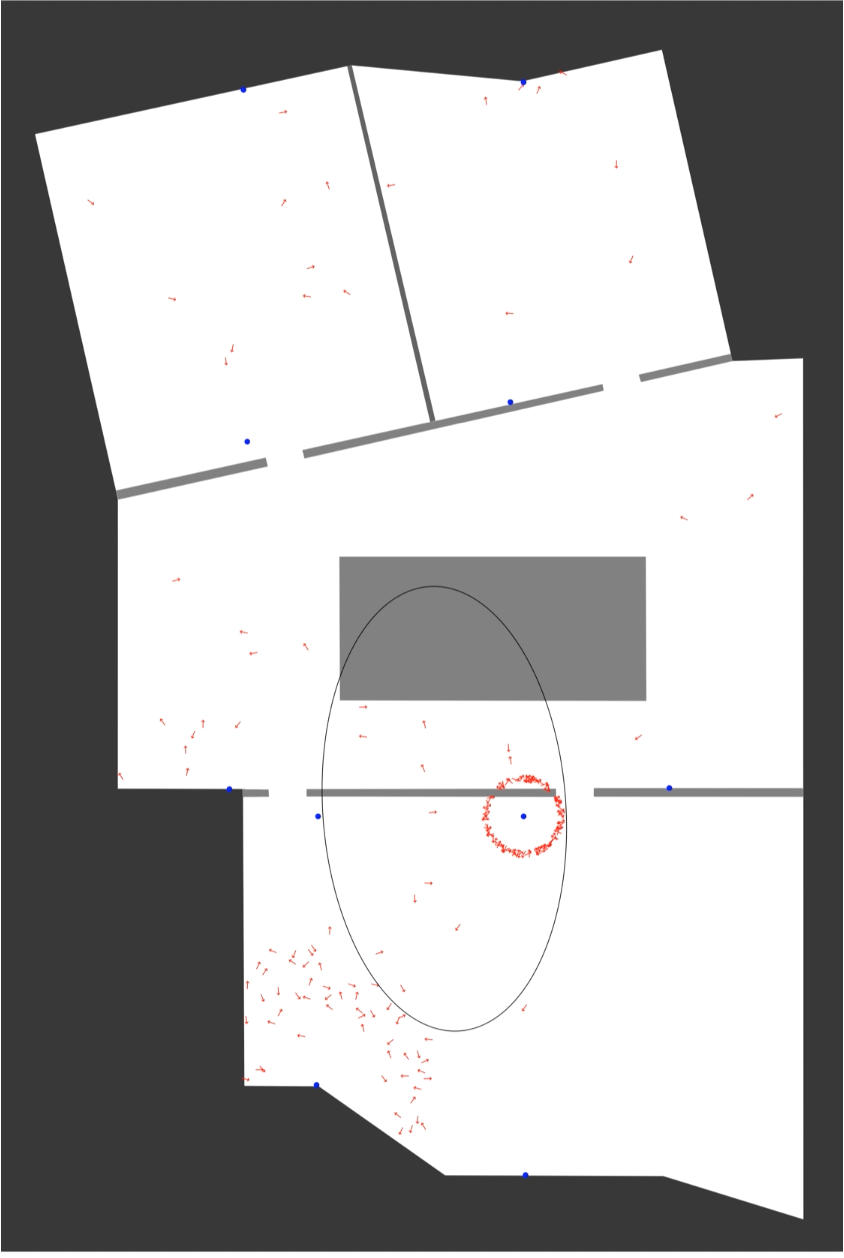
\includegraphics[height=0.7\textwidth]{figures/algo_particle_generation}
\caption{Depicts the initial posterior belief, resp.\ the initial particle set. Particles are shown as red arrows, the beacons as blue filled circles. The large black circle is the $1\sigma$-ellipse.}
\label{fig:pf_initialDist}
\end{figure}

Before the \ac{PF} can start to continuously run, the initial posterior belief $\chi_0$, i.e.\ the particle set, needs to be generated. Tests showed, that a static particle set size of 200~particles is sufficient. As mentioned in chapter~\ref{chap:ibeacons}, each of the beacons can be uniquely identified, by combining the beacon's three identifiers. In addition, their position on the map, i.e.\ the local coordinate system, is known. Consequently, this information can be used to specifically distribute the initial particles around the received beacons. This is a huge advantage, instead of uniformly distributing them on the map's free space. For that reason, the implementation starts ranging for beacons and then wait's, until \ac{CL} reports the first ranged beacons. Then, the particles are distributed in a circle around the beacons, with radius of the estimated distance to that beacon. To take the distance estimation's uncertainty into account, each distance of a particle to its beacon gets added some Gaussian noise with $\mu = 0$ and $\sigma = 0.2 * d$, which depends on the estimated distance $d$. 

Additionally, the amount of particles being spread around a beacon, depends on the estimated proximity. 50\% of the particle set's size are spread around the beacon, which is most probably the closest one to the smartphone, according to its measured proximity. Around the second closest 25\%, the third 12.5\%, \ldots are being spread. The beacon which's proximity is furthest from the smartphone, gets the remaining particles.

The particles are generated with a random orientation $\theta$ where $\theta = [0, 2\pi)$. Figure~\ref{fig:pf_initialDist} shows a screenshot of the implemented iOS app, depicting the initial particle set. The particles are depicted as small red arrows, the beacons as blue filled circles. The black large circle shows the $1\sigma$~ellipse, which gets explained in section~\ref{sec:algo_locEstimation}.


\subsection{Motion Integration}
The \texttt{integrateMotion} function, shown in listing~\ref{lst:algorithmIntegrateMotion}, is a helper function to reduce the complexity of the later introduced algorithm. It gets passed the current particle set $\chi_{t-1}$ and the motion $u_t$ which it applies to each particle. Thus, it samples from the motion model, as discussed in section~\ref{sec:algo_sample_motion}. In the end, it returns the new particle set $\chi_t$.

\begin{lstlisting}[
  float,
  floatplacement=P,
  mathescape,
  captionpos=b,
  caption={Helper function to apply the motion~$u_t$ to the particle set~$\chi_{t-1}$ by sampling from the motion model.},
  label=lst:algorithmIntegrateMotion]
integrateMotion($\chi_{t-1}$, $u_t$) {

  $\bar{\chi}_t = \emptyset$

  for $m = 1$ to $M$ {
    $x^{[m]}_t$ = sample_motion_model($u_t$, $x^{[m]}_{t-1}$)
  }
  return $\bar{\chi}_t$
}
\end{lstlisting}



\subsection{Filtering}
The \texttt{filter} function is another helper function, which is responsible for the \emph{importance factoring} and the \emph{resampling}, depicted in listing~\ref{lst:algorithmSimpleFilter}. It gets passed the particle set $\chi_{t-1}$, the measurements $z_t$ and the \texttt{map}. Then it determines the importance factor of each particle, as explained in section~\ref{sec:algo_measurement_model}. Afterwards, the resampling takes place, to transform the old distribution into the new posterior distribution, as described in section~\ref{sec:fund_pf}. The solution uses \emph{roulette wheel resampling}, which is a common resampling method based on \emph{independent sampling}, proposed by \citet[p. 108--111]{thrun:prob_robo}.

The shown implementation is the basic implementation which does not solve the kidnapping problem. To better understand the implementation, the \acs{PF}'s complexity was reduced, by first showing a simplified filter function, which neglects the recovery. Later in the chapter, the shown \texttt{filter} function is being enhanced, to explain the implemented recovery feature.

\begin{lstlisting}[
  float,
  floatplacement=H,
  mathescape,
  captionpos=b,
  caption={Helper function for the importance factoring and resampling.},
  label=lst:algorithmSimpleFilter]
filter($\chi_{t-1}$, $z_t$, map) {

  $\bar{\chi}_t = \emptyset$

  // importance factoring
  for $m = 1$ to $M$ {
    $w^{[m]}_t$ = measurement_model($z_t$,$x^{[m]}_t$, map)
    add $\langle x^{[m]}_t, w^{[m]}_t \rangle$ to $\bar{\chi}_t$
  }

  $\chi_t = \emptyset$

  \\ resampling
  while size of $\chi_t$ less $M$ {
    draw $i$ with probability $\propto w^{[m]}_t$
    add $x^{[i]}_t$ to $\chi_t$
  }

  return $\chi_t$
}return\end{lstlisting}



\subsection{\acl{PF}}
After explaining all prerequisites, this section gives a detailed insight into the solution's \acl{PF} implementation. To reduce complexity, the \acs{PF}'s code is spit up into three logical parts, shown in listing~\ref{lst:algorithmParticleFilter_1}, \ref{lst:algorithmParticleFilter_2} and \ref{lst:algorithmParticleFilter_3}. Listing~\ref{lst:algorithmParticleFilter}, indicates their call order. It also contains several instance variables, which are accessible from the three parts.

The \texttt{particleFilter} function is continuously being called every $\approx$~1s, if new measurements are available. To remember, \ac{CL} calls its delegate to update the ranged beacons, whether it received a beacon's signal, or not. Consequently, when the function gets called, the latest measurements are always available and ready for processing. It gets passed the particle set $\chi_{t-1}$ and returns the set $\chi_t$.

The implementation uses a static particle set size of 200~particles. Tests showed, that 200~particles are sufficient and increasing the particle set does not really improve the estimation. The \texttt{particleFilter} function requires for one execution on average $\approx$~10ms. Thus, a dynamic particle set size to safe processing power is also not required.

\begin{lstlisting}[
  float,
  floatplacement=H,
  mathescape,
  captionpos=b,
  caption={Shows the \acl{PF}'s implementation and the used instance variables. To reduce complexity the code is divided into three parts, shown in Listing~\ref{lst:algorithmParticleFilter_1}, \ref{lst:algorithmParticleFilter_2} and \ref{lst:algorithmParticleFilter_3}.},
  label=lst:algorithmParticleFilter]
// instance variables
u_buffer // list of not jet integrated motions $u_t$
$u_\text{latest}$ // stores the latest motion
z_buffer // list of not jet integrated measurements $z^{[k]}_t$
map // occupancy grid and landmarks

particleFilter($\chi_{t-1}$) {

  $\bar{\chi}_t = \chi_{t-1}$

  $\bar{\chi}_t$ = PART_1($\bar{\chi}_t$)

  $\bar{\chi}_t$ = PART_2($\bar{\chi}_t$)

  $\bar{\chi}_t$ = PART_3($\bar{\chi}_t$)

  return $\chi_t$
}
\end{lstlisting}



\subsubsection*{Instance Variables}
As mentioned, the motions and measurements are delivered asynchronously by their frameworks. The motion model's implementation already reduces this problem by combining the two headings and the estimated walked distance into one motion. Thus, the \acs{PF}'s implementation has just to deal with two asynchronous sources. To overcome the asynchrony, the motions $u$ and measurements $z$ are buffered in two ascending ordered lists, the \texttt{u\_buffer} and \texttt{z\_buffer}, according their timestamps. The stored motions and measurements, are provided by the motion model and the measurement model, and defined as mentioned in section~\ref{sec:algo_motion_model} and section~\ref{sec:algo_measurement_model}. The instance variable $u_\text{latest}$ stores, as the name already implies, the latest motion that was calculated by the motion model. The \texttt{map} variable stores the environment's map in form of a occupancy grid, and the beacons' positions together with their unique identifiers.


\subsubsection*{\acl{PF} Function --- Part 1}
The algorithm's first part, shown in listing~\ref{lst:algorithmParticleFilter_1}, consists of basically one loop, which tries to integrate the buffered motions and to filter with the buffered measurements at the right point in time. The loop is executed as long as both buffers are not empty. The four if-cases are visualized in figure~\ref{fig:algo_pf_1}. In each example, the \texttt{u\_buffer} contains two motions $u_0, u_1$, and \texttt{z\_buffer} contains one measurement $z_0$. Each subfigure illustrates only the loop's first iteration. Thus, $u_1$ is not relevant during this iteration.

\begin{itemize}
\item{Case 1} (fig.\ \ref{fig:algo_pf_1_1}): If a motion ends before the measurement was taken ($u.{t_\text{end}} < z.t$), the motion is being integrated and $z$ is reserved for the next iteration.

\item{Case 2} (fig.\ \ref{fig:algo_pf_1_2}): If a measurement is taken exactly at the end of a motion ($u.{t_\text{end}} = z.t$), the motion is integrated. Afterwards, the set is filtered with the measurement.

\item{Case 3} (fig.\ \ref{fig:algo_pf_1_3}): If a measurement is taken during a motion ($u.{t_\text{start}} < z.t < u.{t_\text{end}}$), the motion needs to be split-up. The first sub motion is then being integrated into the particle set. Afterwards, it is filtered. The second sub motion is stored in the buffer at the first place, for being processed during the loop's next iteration.

\item{Case 4} (fig.\ \ref{fig:algo_pf_1_4}): If the measurement was taken before the motion ($u.{z.t < t_\text{start}}$ / \texttt{else}), the filter is executed without integrating the motion. The motion is kept back for the next iteration.

\end{itemize}

\noindent If one of the buffers is empty, the algorithm continues with the function's second part.

\begin{lstlisting}[
  float,
  floatplacement=H,
  mathescape,
  captionpos=b,
  caption=Shows the \texttt{particleFilter} function's first part.,
  label=lst:algorithmParticleFilter_1]
PART_1($\chi_{t-1}$) {

  $\bar{\chi}_t = \chi_{t-1}$

  while u_buffer isNotEmpty && z_buffer isNotEmpty {
    $u$ = u_buffer.first
    $z$ = z_buffer.first
    if $u.{t_\text{end}}$ < $z.t$ {
      $\bar{\chi}_t$ = integrateMotion($\bar{\chi}_t$, $u$)
      u_buffer.remove($u$)
    } else if $u.{t_\text{end}} = z.t$ {
      $\bar{\chi}_t$ = integrateMotion($\bar{\chi}_t$, $u$)
      $\bar{\chi}_t$ = filter($\bar{\chi}_t$, $z$, map)
      u_buffer.remove($u$)
      z_buffer.remove($z$)
    } else if $u.{t_\text{start}} < z.t$ && $z.t < u.{t_\text{end}}$ {
      split $u$ at timestamp $z.t$ in $u_1$ and $u_2$
      $\bar{\chi}_t$ = integrateMotion($\bar{\chi}_t$, $u_1$)
      $\bar{\chi}_t$ = filter($\bar{\chi}_t$, $z$, map)
      u_buffer.remove($u$)
      insert $u_2$ at beginning of u_buffer
      z_buffer.remove($z$)
    } else {
      $\bar{\chi}_t$ = filter($\bar{\chi}_t$, $z$, map)
      z_buffer.remove($z$)
    }
  }

  return $\bar{\chi}_t$
}
\end{lstlisting}


\begin{figure}
	\subfloat[Case: $u.{t_\text{end}} < z.t$]{
  \begin{tikzpicture}
    \draw[->] (0,1) -- (6,1);
      \draw (6.5,1)node(y){$t$};

      \draw[blue] (1,2)--(3,2);
      \draw[blue] (2,2.5)node(a){$u_0$};

      \draw[red, dashed] (3,2)--(5,2);
      \draw[red] (4,2.5)node(a){$u_1$};

      \draw (4,1)--(4,0.5);
      \draw (4,0)node(a){$z_0$};
  \end{tikzpicture}
  \label{fig:algo_pf_1_1}
}
\subfloat[Case: $u.{t_\text{end}} = z.t$]{
  \begin{tikzpicture}
    \draw[->] (0,1) -- (6,1);
      \draw (6.5,1)node(y){$t$};

      \draw[blue] (1,2)--(3,2);
      \draw[blue] (2,2.5)node(a){$u_0$};

      \draw[red, dashed] (3,2)--(5,2);
      \draw[red] (4,2.5)node(a){$u_1$};

      \draw (3,1)--(3,0.5);
      \draw (3,0)node(a){$z_0$};
  \end{tikzpicture}
  \label{fig:algo_pf_1_2}
}

\subfloat[Case: $u.{t_\text{start}} < z.t < u.{t_\text{end}}$]{
  \begin{tikzpicture}
    \draw[->] (0,1) -- (6,1);
      \draw (6.5,1)node(y){$t$};

      \draw[blue] (1,2)--(3,2);
      \draw[blue] (2,2.5)node(a){$u_0$};

      \draw[red, dashed] (3,2)--(5,2);
      \draw[red] (4,2.5)node(a){$u_1$};

      \draw (2,1)--(2,0.5);
      \draw (2,0)node(a){$z_0$};
  \end{tikzpicture}
  \label{fig:algo_pf_1_3}
}
\subfloat[Case: \texttt{else}]{
  \begin{tikzpicture}
    \draw[->] (0,1) -- (6,1);
      \draw (6.5,1)node(y){$t$};

      \draw[blue] (1,2)--(3,2);
      \draw[blue] (2,2.5)node(a){$u_0$};

      \draw[red, dashed] (3,2)--(5,2);
      \draw[red] (4,2.5)node(a){$u_1$};

      \draw (0.5,1)--(0.5,0.5);
      \draw (0.5,0)node(a){$z_0$};
  \end{tikzpicture}
  \label{fig:algo_pf_1_4}
}

	\caption{Visually illustrates the four cases shown in listing~\ref{lst:algorithmParticleFilter_1}.}
	\label{fig:algo_pf_1}
\end{figure}


\subsubsection*{\acl{PF} Function --- Part 2}
If after executing the first part still motions are buffered, these motions are being integrated in this part. The reason for the remaining motions is, that \texttt{particleFilter} function is also being called if no measurements are received, as mentioned at the beginning. The reason why they can be integrated without current measurements is, they are definitely older than the not yet occurred measurements and thus there is no reason to keep them back.

After integrating a motion, the filter method is called. The filtering is executed without an actual measurement. Thus, only the map's occupancy grid is used to calculate the particle's importance factors. Consequently, particles that are moved onto an occupied position, are sorted out.

The purpose of not waiting for the next measurement to integrate the remaining motions is on one hand, that if the user is out of the beacons range, the motion is still being integrated; thus, the particles on the view are still moving according to the users motion. On the other hand the algorithms performance does not get worse, because \texttt{u\_buffer} never contains more motion's that need to be integrated, as in general.

\begin{lstlisting}[
  float,
  floatplacement=H,
  mathescape,
  captionpos=b,
  caption=Shows the \texttt{particleFilter} function's second part.,
  label=lst:algorithmParticleFilter_2]
PART_2($\chi_{t-1}$) {

  $\bar{\chi}_t = \chi_{t-1}$

  // integrate residual motions, filter just with map
  while u_buffer isNotEmpty {
    $u$ = u_buffer.first
    $z = \emptyset$
    $\bar{\chi}_t$ = integrateMotion($\bar{\chi}_t$, $u$)
     u_buffer.remove($u$)

     // filter without measurements, just with map
     $\bar{\chi}_t$ = filter($\bar{\chi}_t$, $z$, map)
  }

  return $\bar{\chi}_t$
}
\end{lstlisting}



\subsubsection*{\acl{PF} Function --- Part 3}
The first two part are important for integrating and filtering while a person is walking. But integrating measurements if a person is stationary can drastically improve the estimated location, as shown in chapter~\ref{chap:evaluation}. Thus, the received measurements are directly integrated, instead of buffering them, as shown in listing~\ref{lst:algorithmParticleFilter_3}. Furthermore, the user sees without a big delay, how the posterior changes by applying the measurements directly.

To be able to integrate them directly, the algorithm needs to be sure that the user is stationary. As mentioned in chapter~\ref{chap:sensors}, \acs{CL} has the problem of requiring 6~--~8~steps to recognize that a person is walking, i.e.\ until it delivers this information. Consequently, if a user is stationary and starts to walk, the measurements collected during the first steps need to be buffered until the motion data is available, otherwise the measurements would be integrated at the wrong position. The second important information is to know, that a person is now stationary, and no further motions are being delivered. Only then, the measurements can directly, without delay, being integrated.

The latter problem can be solved easily. Motions are delivered every $\approx$~2.5s. Thus, if the difference between now and the latest motion $u_\text{latest}$ is at least 2.7s, \acs{CM} does not deliver any new motion until the person starts to walk again. 2.7s was chosen, because the 2.5s are an approximate value. Besides that the \texttt{particleFilter} function is only called every $\approx$~1s, thus no additional delay is being created.

To be able to buffer the measurements during the first steps, when the user starts to walk again, the solution presented in section~\ref{sec:algo_stationary}, is used. Due to the solution's simple moving average over the last one second, it detects within $\approx$~1s if a user is stationary or not. Thus, if the user is not stationary, the motion integration is not executed, and the values are kept in the buffer.

Furthermore, tests showed, that by additionally integrating a small Gaussian distributed random motion with $\sigma = 0.3m$, helps to faster improve the location accuracy. If a person is stationary, the person's orientation does not matter. Consequently, also the motion's orientation $\theta$ is set to a uniformly distributed random value between $[0, 2 \cdot \pi)$. Using a random orientation has the advantage, that the particles can move in any direction.

\begin{lstlisting}[
  float,
  floatplacement=H,
  mathescape,
  captionpos=b,
  caption={Part 3 of the solution's \texttt{particleFilter} function shown in Listing~\ref{lst:algorithmParticleFilter}.},
  label=lst:algorithmParticleFilter_3]
PART_3($\chi_{t-1}$) {

  $\bar{\chi}_t = \chi_{t-1}$

  $\Delta t$ = currentDate - $u_\text{latest}.t_\text{end}$ // in seconds

  if motionModel.deviceIsStationary && $\Delta t \le 2.7$  {
    $u$ = motion with distance $0.0$
    $z$ = z_buffer.first

    $\bar{\chi}_t$ = integrateMotion($\bar{\chi}_t$, $u$)
    $\bar{\chi}_t$ = filter($\bar{\chi}_t$, $z$, map)
    z_buffer.remove($z$)
  }

  return $\bar{\chi}_t$
}
\end{lstlisting}



\subsection{Recovery / Kidnapping Problem}\label{sec:algo_recovery}
The implemented recovery feature has two purposes. Firstly, it can happen, that all particles are moving out of bounds, and thus, are being filtered out. Secondly, if the particles are on a totally wrong position, which can happen if the user walked to soft, and thus the pedometer could not recognize the user's steps. It can also happen that the orientation does not fit the actual one; for instance, the user's phone points not straight forward during the walk.

To determine both situations, the before introduced \texttt{filter} function, shown in listing~\ref{lst:algorithmSimpleFilter}, was enhanced to support recovery. The enhanced version is shown in listing~\ref{lst:algorithmFilter}. During the resampling, the new particle set's \texttt{weightSum}~=~$\sum_{m = 0}^{M-1} w^{[m]}_t$, which is the sum of all drawn particles, during the resampling, is calculated.

If the $\texttt{weightSum} == 0$, $\chi_t$ is empty, thus all particles are moved out of bounds or their location is already occupied, and thus are being ignored. Consequently, a new random particle set is being generated. The particles are distributed as described in section~\ref{sec:algo_initial}, i.e\ the position estimation is restarted.

If the $\texttt{weightSum} > 0$, it gets normalized by the particle sets size. Then, it is stored in the \texttt{particleSums} array, which contains the latest three weightSums (line 24). When the \texttt{filter} function is called the next time, it first checks if the array already contains three weight sums, and if true, the average of the three weight sums is calculated (line 8). If the average drops below a certain threshold (set to 1.0), it is very likely, that the posterior's distribution does not match the user's true position, i.e.\ it is totally wrong. To recover from this state 20\% additional random particles where added to the particle set. The random particles are distributed as described in section~\ref{sec:algo_initial}. Due to the fact, that the particles are being added before the importance factoring and resampling, the added particles help to recover from the state, by getting higher importance factors, and thus they are drawn with a high probability.

Test of different random particle counts showed, that 20\% seems to bring the best result. Adding to less particles does not really help to recover, but adding to much results in a heavily jumping position estimation. The reason for taking the average over the last three weight sums is, that sometimes the weight sum drastically drops during one filter call. This happens for instance, if the measurements to the beacons where heavily influenced by an obstacle, and thus are totally wrong.

Figure~\ref{fig:algo_recovery} illustrates the recovery. The shown weight sums correspond to the two screenshots. During the experiment, the kidnapping problem was simulated by walking very smooth, approximately on the green path, from the lower lecture hall through the building's foyer, by passing the large obstacle at the left side, into the upper right lecture hall. After being their stationary for a few seconds, we returned, by passing the obstacle on the other side. During the walk, the iPhone's pedometer was not able to recognize any step. Both experiments, the one with recovery (fig.~\ref{fig:algo_recovery_withRecovery}) and the one without recovery (fig.~\ref{fig:algo_recovery_withoutRecovery}), are simulated by using the exact same recorded data, as input.

By testing different thresholds in different scenarios, a threshold of 1.0 seems fit best. In this example recovery was being executed the first time after $\approx$~90s. During the long break from 60s~--~90s the test user walked through the foyer, where no beacons with an estimated distance of less than 5m where ranged. Thus the \texttt{filter} function was not executed. After receiving measurements again, the average particle weight sum dropped below the threshold, and recovery took place. Thus, the particles jumped from the lower to the upper lecture hall. The same happened at $\approx$~155s on the way back. The third recovery is executed at $\approx$~184s, which caused a small jump next to the end position.

Without recovery, shown in figure~\ref{fig:algo_recovery_withoutRecovery}, the algorithm is not able to approximate the true location. After $\approx$~90s the weight sum drops to $\approx$~0, and stays there.


\begin{lstlisting}[
  float,
  floatplacement=H,
  mathescape,
  captionpos=b,
  caption={Depicts the solution's enhanced filter function including recovery},
  label=lst:algorithmFilter]
// instance variable
weightSums // array that stores the last 3 weight sums

filter($\chi_{t-1}$, $z_t$, map) {

  $\bar{\chi}_t = \emptyset$

  if size of weightSum == 3 && avg.\ weightSums < 1.0 {
    add $0.2\%$ additional random particles to $\chi_{t-1}$
  }

  // importance factoring
  $\ldots$

  weightSum = $0.0$

  \\ resampling
  while size of $\chi_t$ less $M$ {
    $\ldots$
    weightSum += $w^{[m]}_t$
  }

  if weightSum > 0 {
    override oldest value in weightSum with (weightSums/particleSetSize)
  } else {
    $\chi_t$ = generate new random particle set
    clear weightSums
  }
  return $\chi_t$
}return\end{lstlisting}


\begin{figure}
	\subfloat{
  \begin{tikzpicture}
    \begin{axis}[trim axis left, trim axis right, width=0.9\textwidth, height=0.4\textheight,
      xlabel={Time (sec)},
      ylabel={ParticleWeightSum},
      legend entries={with recovery, without recovery},
      grid = major]
      \addplot [red, mark=x] table[col sep=semicolon, x=timestamp, y=normalizedWeightSum] {csv/F-Foyer2_F007-F023-F007_kidnapping/ParticleWeight_withRecovery.csv};
      \addplot [blue, mark=x] table[col sep=semicolon, x=timestamp, y=normalizedWeightSum] {csv/F-Foyer2_F007-F023-F007_kidnapping/ParticleWeight_withoutRecovery.csv};
    \end{axis}
  \end{tikzpicture}
}

\subfloat[with recovery] {
  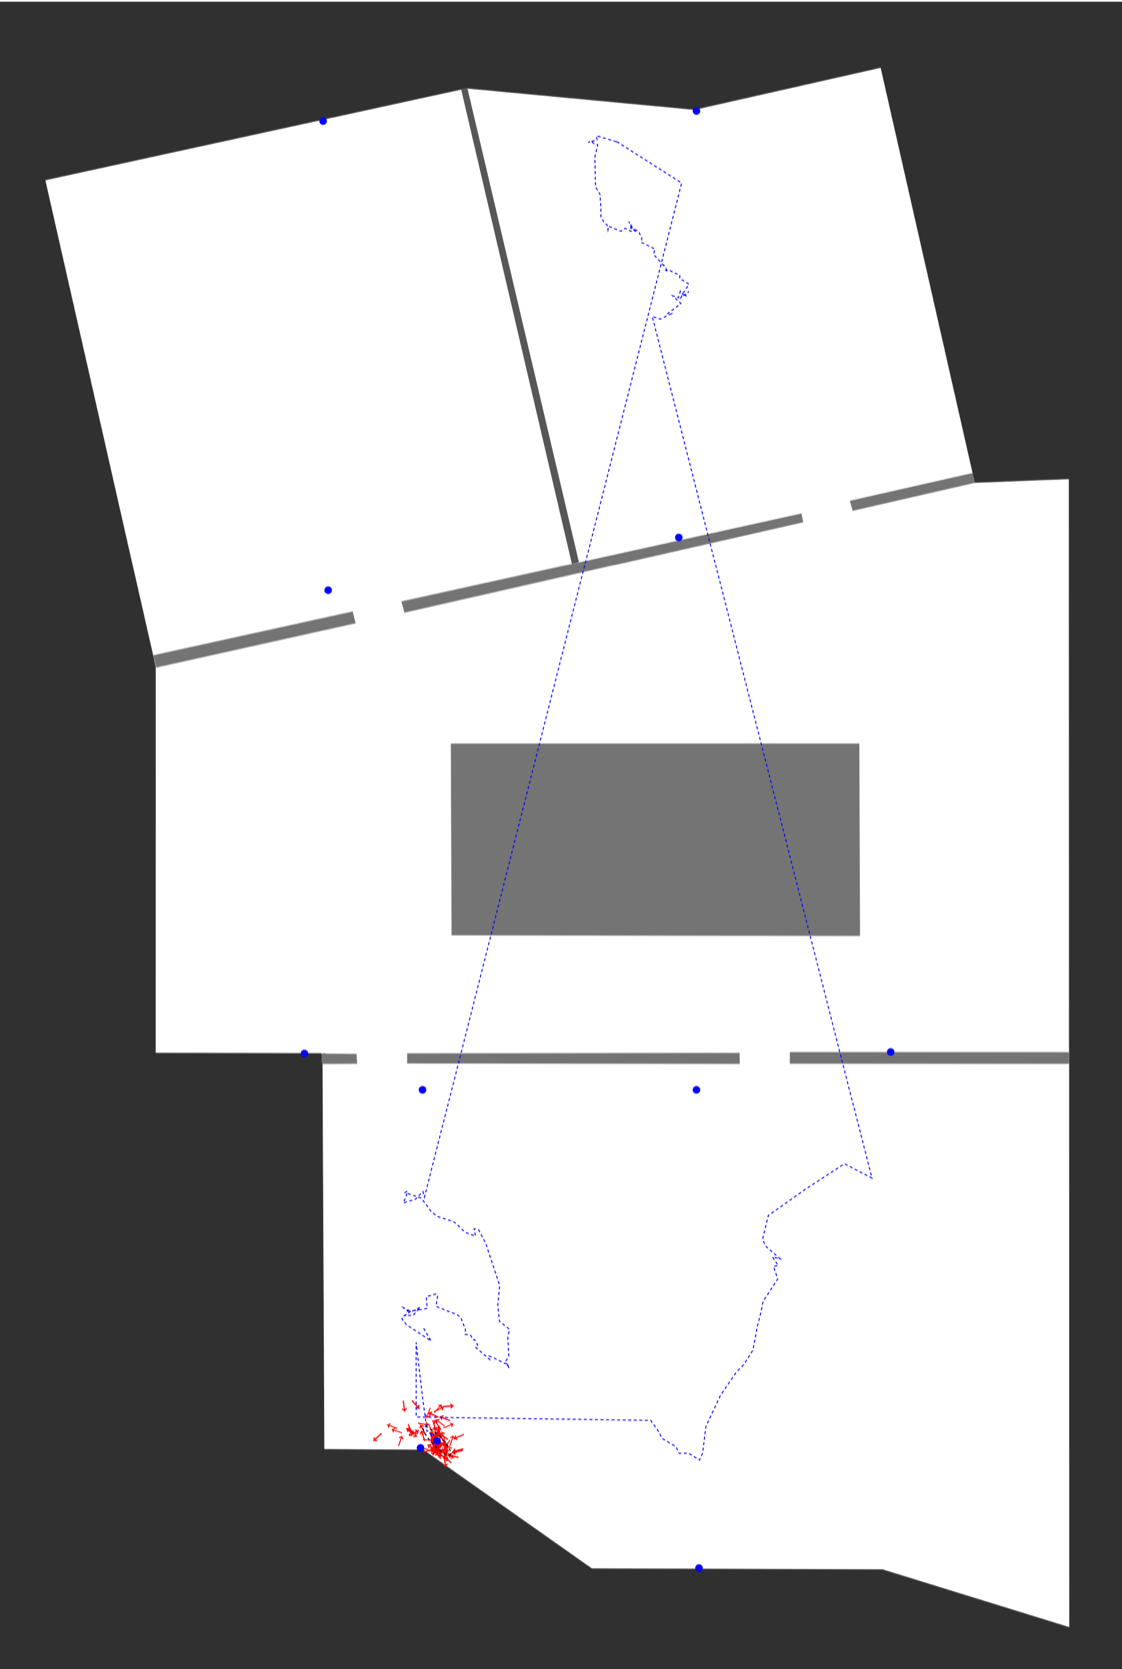
\includegraphics[height=0.5\textheight]{figures/algo_withRecovery}
  \label{fig:algo_recovery_withRecovery}
}
\subfloat[without recovery] {
  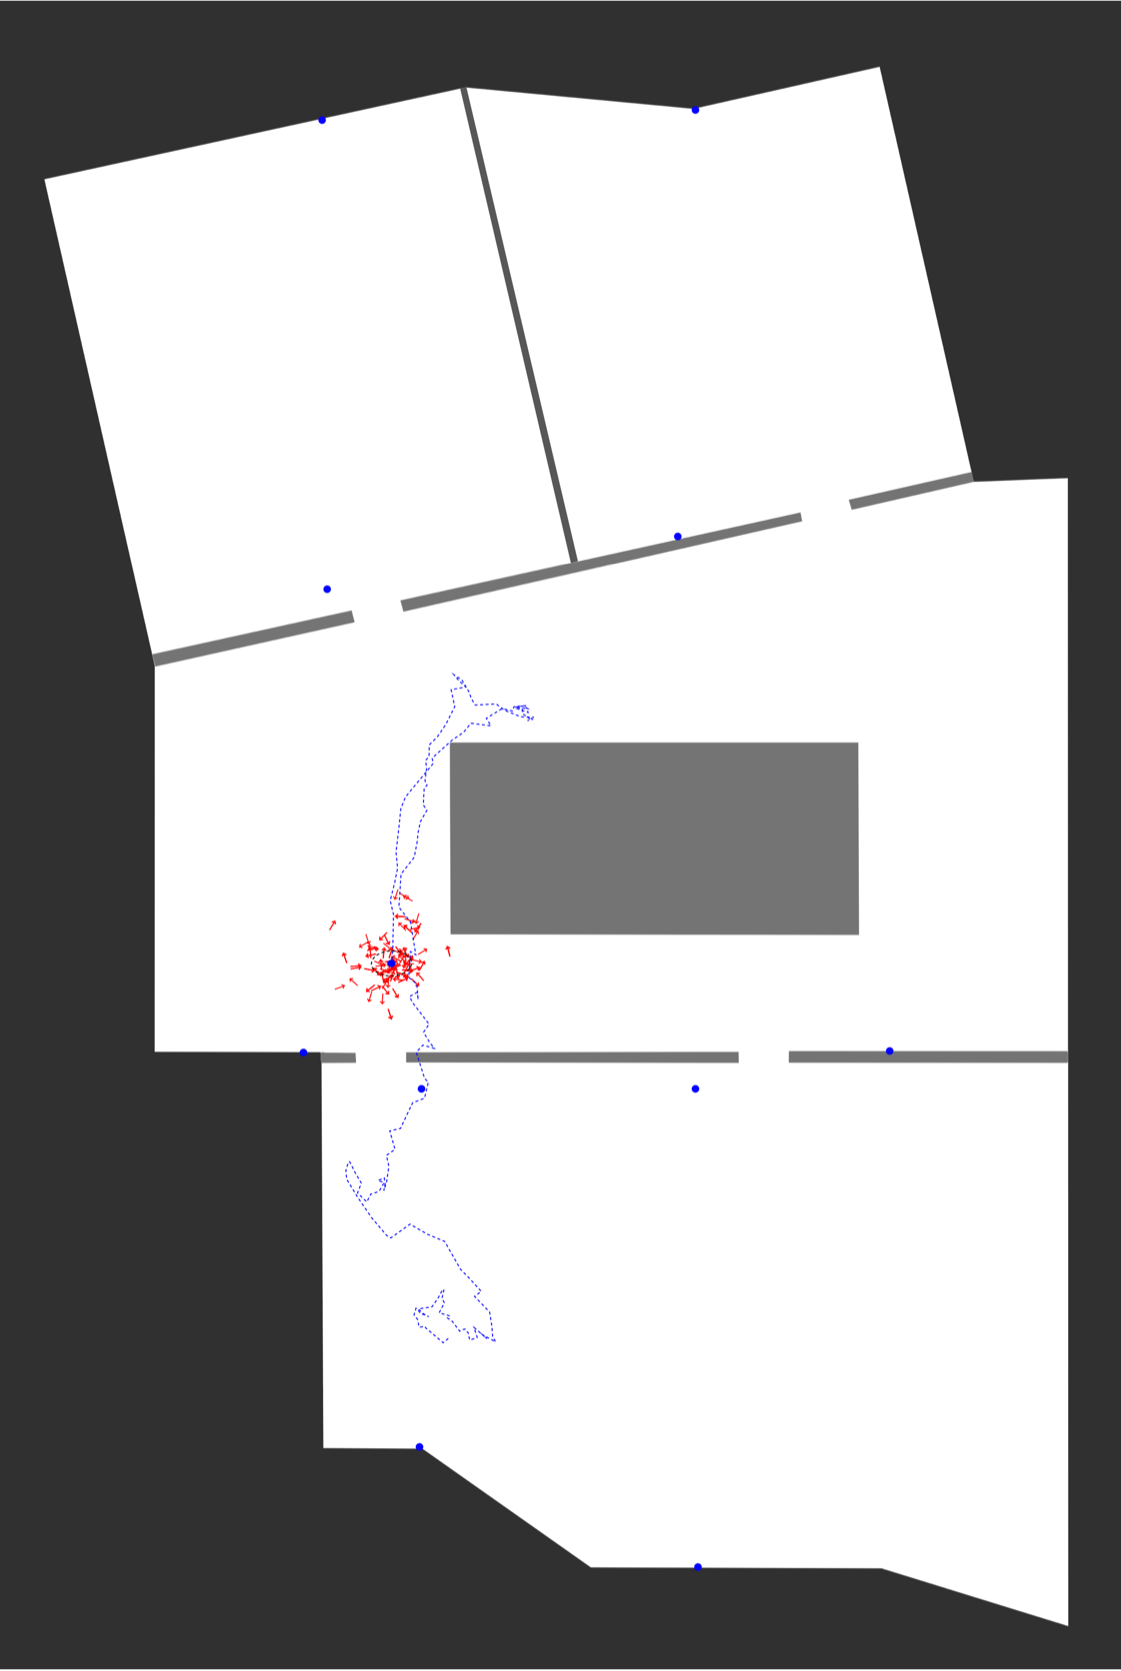
\includegraphics[height=0.5\textheight]{figures/algo_withoutRecovery}
  \label{fig:algo_recovery_withoutRecovery}
}

	\caption {Depicts an example with and without the solution's recovery feature.}
	\label{fig:algo_recovery}
\end{figure}

\subsection{Location Estimation}\label{sec:algo_locEstimation}
To be able to display a concrete location estimation instead of a particle cloud, the \acs{PF}'s posterior belief, which is a multi-modal distribution, represented by the particle set $\chi_t$, needs to be converted into another distribution. As mentioned in chapter~\ref{chap:fundamentals}, uncertainties are typically modeled as Gaussians. Consequently, it is applicable to transform the \acs{PF}'s posterior into a two-dimensional gaussian $N(\mu, \Sigma)$, where the mean $\mu = (x, y)^T$ represents the concrete location. The location's uncertainty is expressed as the covariance matrix $\Sigma = \bigl(\begin{smallmatrix} \sigma_{x}^2&\sigma_{xy}\\ \sigma_{yx}&\sigma_{y}^2 \end{smallmatrix} \bigr)$.

The mean $\mu$, can either be $\chi$'s arithmetic mean or its weighted mean, by using the particle's importance factors as weights. Based on the estimated mean, the covariance $\Sigma$ can be determined. The Gaussian's parameters can then be used to visualize the user's location on the map in form of a $1\sigma\text{-ellipse}$. Thus the user's true location is with a probability of $\approx$~39\%, somewhere in the $1\sigma\text{-ellipse}$. Figure~\ref{fig:algo_sigellipse}, illustrates the transformation of the particle set $\chi$ into a gaussian, shown as $1\sigma\text{-ellipse}$.

\begin{figure}
	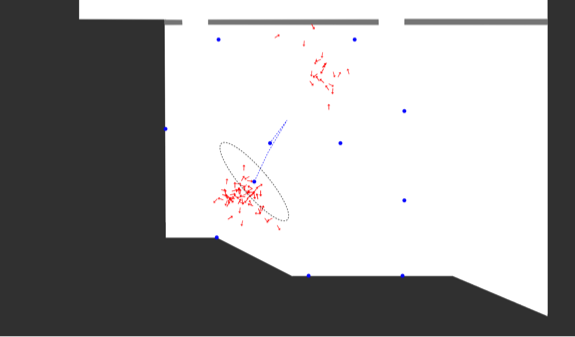
\includegraphics[width=0.7\textwidth]{figures/sigellipse}
	\caption{Depicts the transformation of $\chi$ into a gaussian, shown as $1\sigma\text{-ellipse}$, with a weighted mean.}
	\label{fig:algo_sigellipse}
\end{figure}

\chapter{Evaluation} \label{chap:evaluation}
After presenting our solution for indoor self-localization, we are now going to evaluate the in chapter~\ref{chap:pf} presented implementation, based on the criteria according to \citet{IEEE:survey_wireless_indoor_pos}, introduced in section~\ref{sec:fund_loc}.

\section{Accuracy and Precision}
To determine our solution's accuracy and its precision, we did different tests in a real world experiment. Therefor, we deployed the 10 beacons, we bought from BEACONinside, in parts of a building of our university. We tested it in a static environment; thus, the test person was the only dynamic subject in the experiment. Besides the deployed beacons, the building is also equipped with several WiFi access points, which are also sending on 2.4~GHz, and thus, may influence the bacons's signal's. During the experiments, we used a static particle set size of 200 particles, as mentioned in chapter~\ref{chap:pf}.

\subsection*{Experiment~1}
In our first experiment we equipped just one lecture hall with our 10 beacons. Figure~\ref{fig:f007} shows a picture of the lecture hall, to give a better insight. On the following screenshots, it is depicted on the map's lower part, taken from the lower left corner.

\begin{figure}
	\includegraphics[width=0.9\textwidth]{figures/F007}
	\caption{Shows the lecture hall depicted on the map's lower part.}
	\label{fig:f007}
\end{figure}

\begin{figure}
	\subfloat[Path] {
		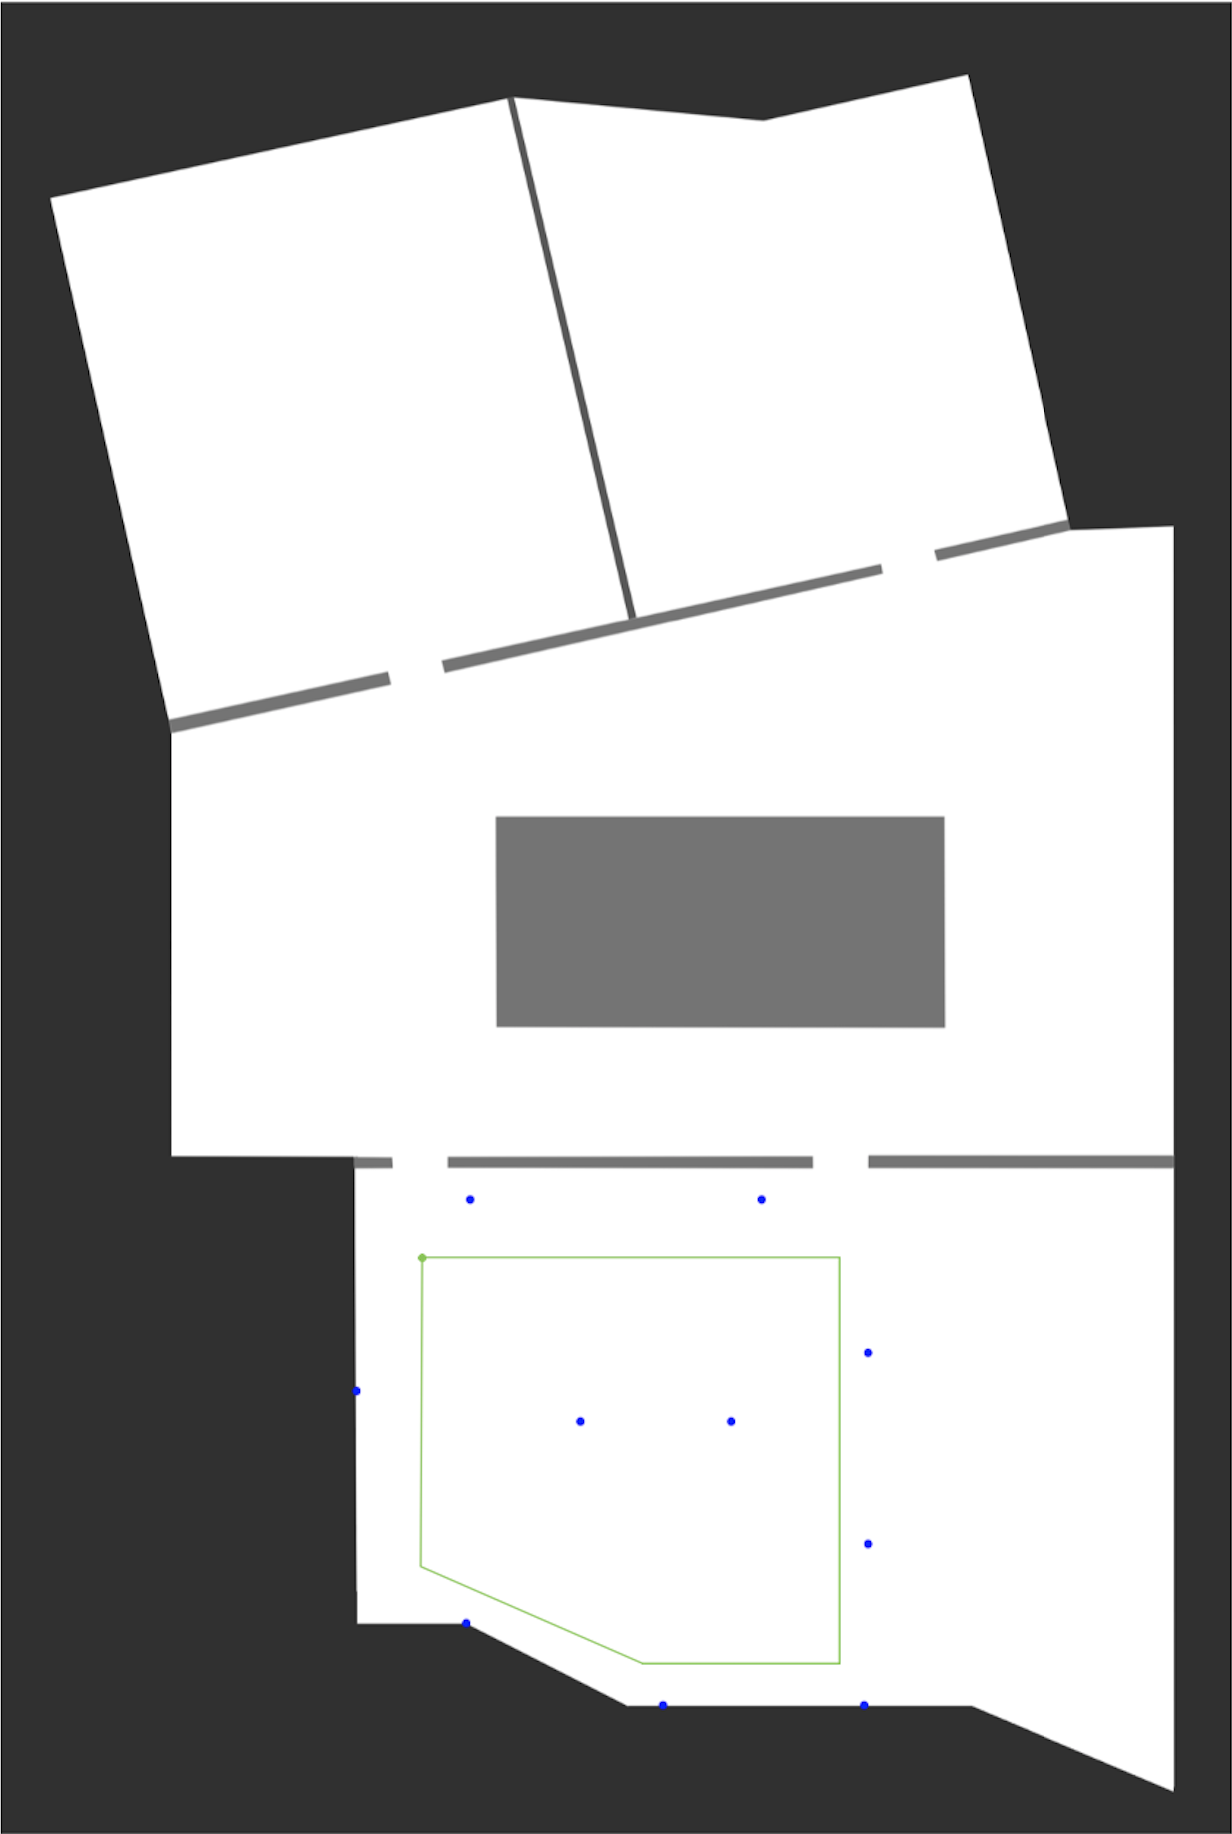
\includegraphics[height=0.45\textheight]{figures/eval_1_path}
		\label{fig:exp1_path}
	}
	\subfloat[] {
		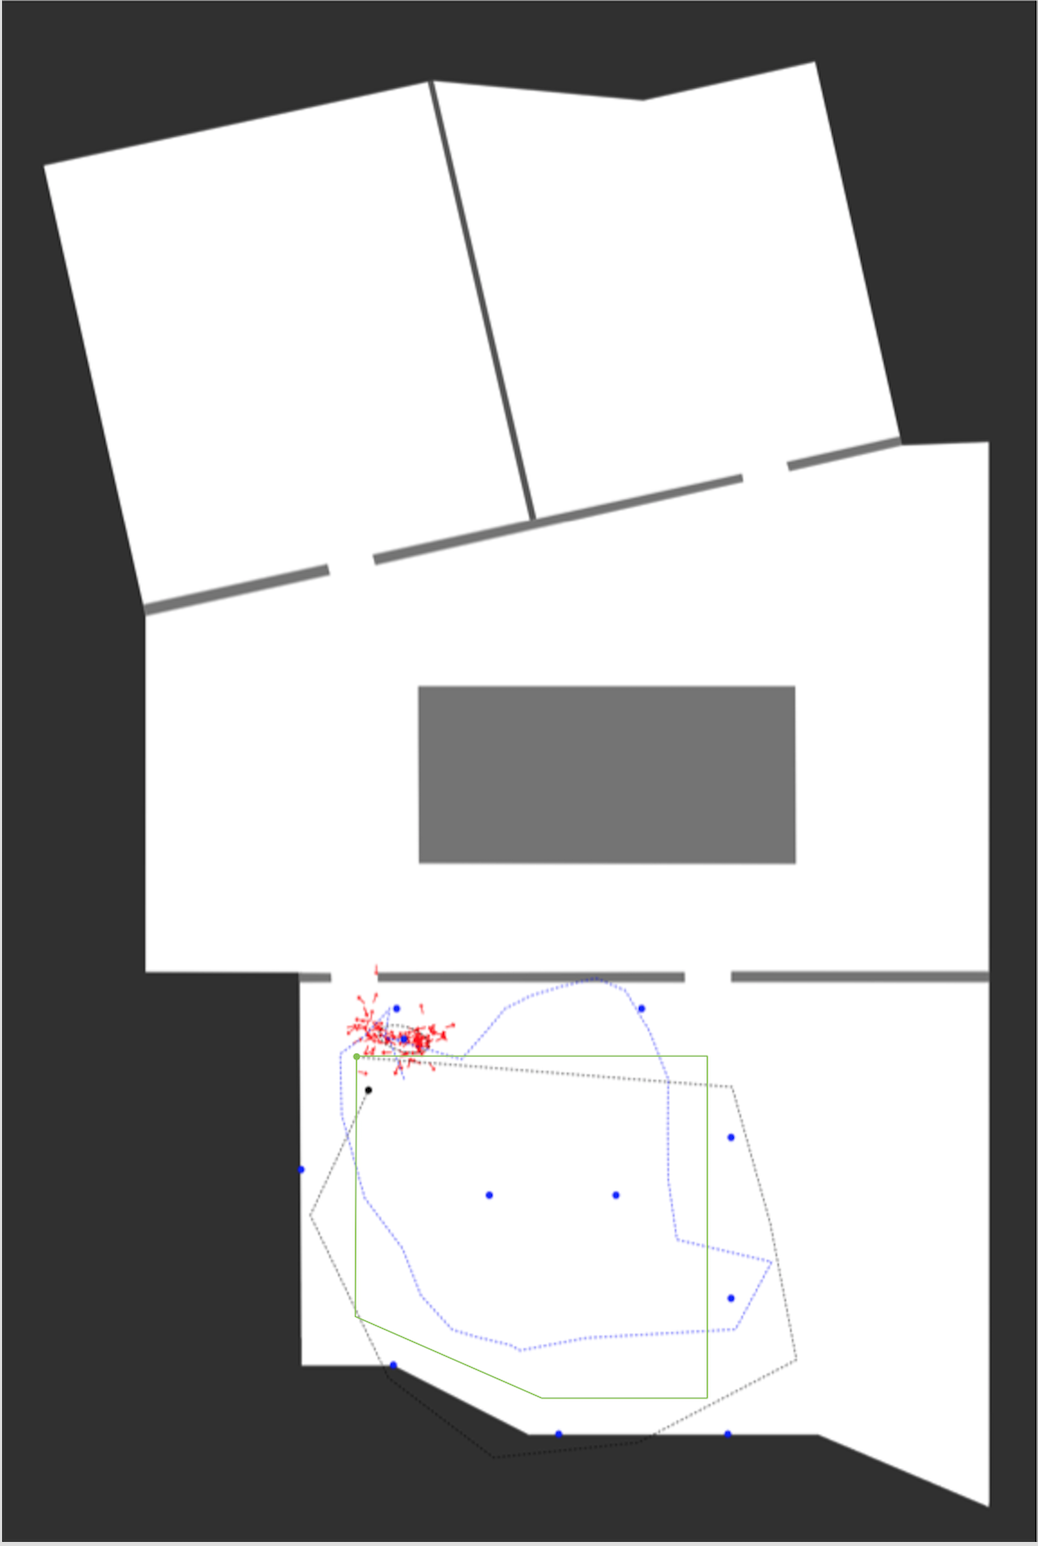
\includegraphics[height=0.45\textheight]{figures/eval_1_1}
		\label{fig:exp1_img_1}
	}
	
	\subfloat[] {
		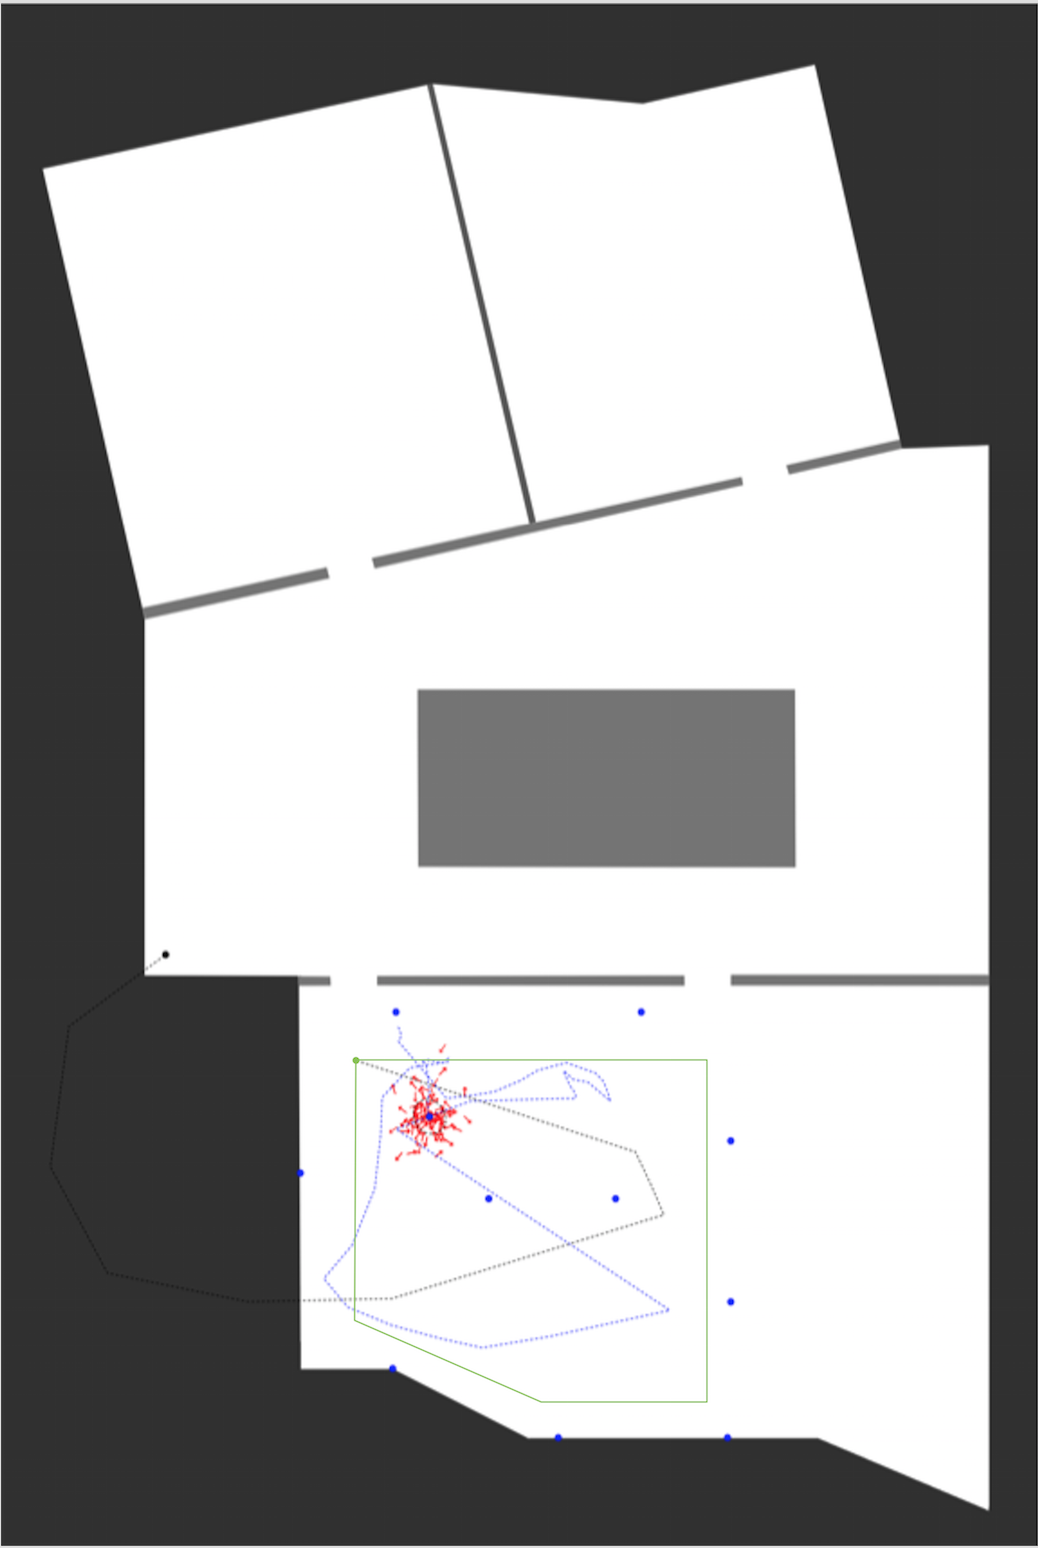
\includegraphics[height=0.45\textheight]{figures/eval_1_2}
		\label{fig:exp1_img_2}
	}
	\subfloat[] {
		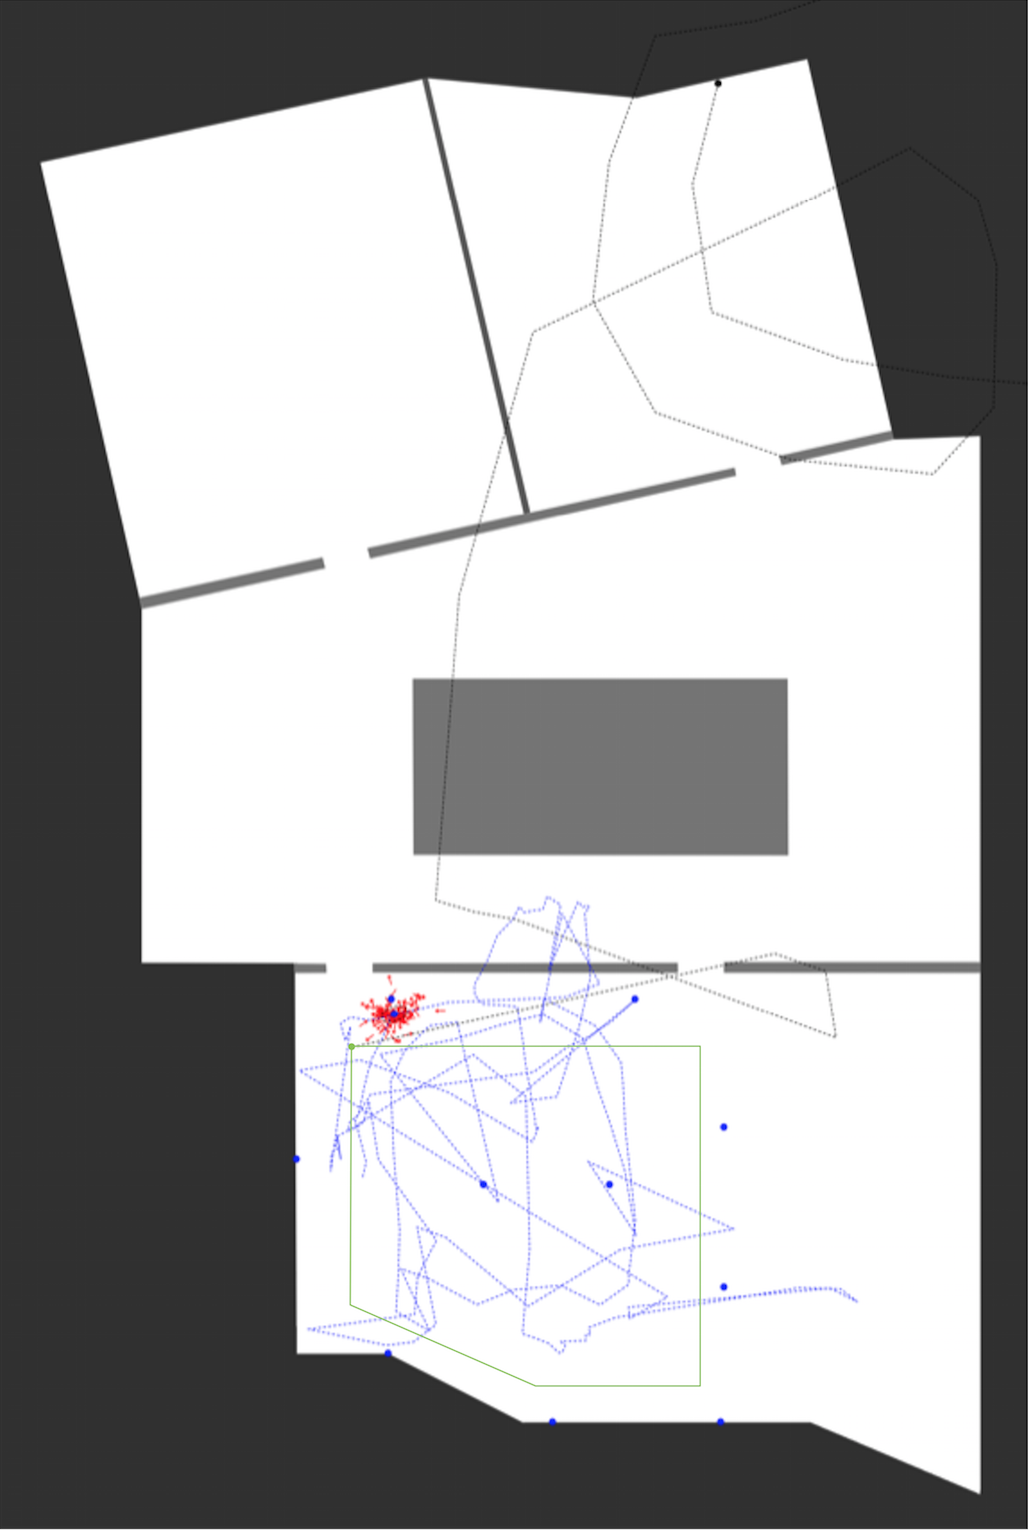
\includegraphics[height=0.45\textheight]{figures/eval_1_3}
		\label{fig:exp1_img_3}
	}
	\caption{Screenshots illustrate some results of Experiment~1.}
	\label{fig:exp1_screenshot}
\end{figure}

During the experiment we tested how good our localization works inside the shown lecture hall. The lecture hall, depicted in the lower part of figure~\ref{fig:exp1_path}, is approx.\ 15~meters long and 8–11 meters wide. The 10 beacons's positions are depicted as blue circles.

To determine the algorithms accuracy, we walked on a specified path, depicted in green, beginning and ending at the upper left corner. At the end of each walk we compared the application's estimated end position with the true end position, by calculating the error, in form of the euclidian distance. As mentioned in section~\ref{sec:algo_locEstimation}, the location can be estimated by either calculating the mean of $\chi$, or by calculating its weighted mean. To be able to compare their results, we calculated the error for both approaches.

Additionally, we calculated the error of the motion tracking's end position with the true position. To be able to compare the motions error with the applications error, by taking the motions drift into account, we split up the experiment in three scenarios. First, we walked just one round on the green path. Second, two rounds and third, three rounds. For each scenario we did three walks in clockwise and three in counter-clockwise direction on the path.

Furthermore, we wanted to find out, if the accuracy improves after being stationary for a short time at the end position. Consequently, we calculated the error for the estimated position directly after integrating the last reported distance, estimated by \ac{CM}'s \texttt{CMPedometer} component, and additionally, $\approx 5~sec$ after integrating the last distance estimation.


\begin{figure}

\subfloat[Error at stop]{
	\begin{tabular}{c||cc|cc}
		Scenario & $\mu$ & $\sigma$ & $\mu_w$ & $\sigma_w$\\
		\hline
		1 & 2.23 & 2.74 & 2.08 & 2.55\\
		2 & 2.16 & 2.53 & 2.16 & 2.53\\
		3 & 3.00 & 3.64 & 3.55 & 4.23\\
		\hline
		1--3 & 2.47 & 2.83 & 2.60 & 3.01\\
	\end{tabular}
	\label{fig:exp1_results_1}
}
\subfloat[Error after $\approx 5~sec$]{
	\begin{tabular}{c||cc|cc}
		Scenario & $\mu$ & $\sigma$ & $\mu_w$ & $\sigma_w$\\
		\hline
		1 & 2.19 & 3.13 & 2.17 & 3.13\\
		2 & 1.94 & 2.52 & 1.95 & 2.53\\
		3 & 2.73 & 3.71 & 2.74 & 3.72\\
		\hline
		1--3 & 2.29 & 2.97 & 2.29 & 2.97\\
	\end{tabular}
	\label{fig:exp1_results_2}
}

\subfloat[Error of motion tracking]{
	\begin{tabular}{c||cc}
		Scenario & $\mu$ & $\sigma$\\
		\hline
		1 & 3.63 & 4.24\\
		2 & 7.11 & 8.05\\
		3 & 10.81 & 13.21\\
		\hline
		1--3 & 7.19 & 13.21\\
	\end{tabular}
	\label{fig:exp1_results_3}
}
\caption{Depicts the results of experiment~1.}
\label{fig:exp1_results}
\end{figure}

\begin{figure}
	\begin{tikzpicture}
	\begin{axis}[trim axis left, trim axis right, height=0.4\textheight,
		xlabel={Scenario},
		ylabel={Error (m)},
		legend entries={$\mu$ (fig.\ \ref{fig:exp1_results_1}), $\mu_w$ (fig.\ \ref{fig:exp1_results_1}), $\mu$ (fig.\ \ref{fig:exp1_results_2}), $\mu_w$ (fig.\ \ref{fig:exp1_results_2}), $\mu$ (fig.\ \ref{fig:exp1_results_3})},
		legend pos=north west,
		grid = major,
		xtick=data]
		\addplot [blue, only marks] table[col sep=semicolon, x=scenario, y=mean] {csv/eval/Eval_1_ep1/NDFScenario.csv};
		\addplot [blue, only marks, mark=square*] table[col sep=semicolon, x=scenario, y=w_mean] {csv/eval/Eval_1_ep1/NDFScenario.csv};
		\addplot [red, only marks] table[col sep=semicolon, x=scenario, y=mean] {csv/eval/Eval_1_ep2/NDFScenario.csv};
		\addplot [red, only marks, mark=square*] table[col sep=semicolon, x=scenario, y=w_mean] {csv/eval/Eval_1_ep2/NDFScenario.csv};
		\addplot [green, only marks] table[col sep=semicolon, x=scenario, y=mean] {csv/eval/Eval_1_motion/NDFScenario.csv};
	\end{axis}
\end{tikzpicture}
\caption{Visualizes the results shown in figure~\ref{fig:exp1_results}.}
\label{fig:exp1_visualization}
\end{figure}

\subsubsection*{Result}
The experiments results are shown in figure~\ref{fig:exp1_results} and are being visualized in figure~\ref{fig:exp1_visualization}.

Figure~\ref{fig:exp1_results_1} depicts the average distance error and the error's spreading, for each scenario, directly after integrating the last motion; whereas, figure~\ref{fig:exp1_results_2} values are being calculating by using the estimated position $\approx 5~\text{sec}$ after the last motion integration. The calculated average error by using $\chi$'s mean, as location, is denoted with $\mu$ and the errors standard deviation is denoted with $\sigma$. $\mu_w$ and $\sigma_w$, are the average error and its standard deviation by using the weighted mean of $\chi$ for the position estimation.
Figure~\ref{fig:exp1_results_3} shows the motion tracking's error $\mu$ and the errors spreading, in form of its standard deviation $\sigma$.

The results show, that during the experiment an accuracy of $2.29~m$ -- $2.6~m$ was achieved. It also shows, that the location estimation, tends to improves after being stationary at the end position, as expected.

The difference of the two position estimation approaches, is very small. The result sways, sometimes $\chi$'s mean, and sometimes its weighted mean is more accurate. We assume, that the minimal difference is based on the particle cloud's high concentration.

The result's visualization also clearly states, that the motion's error grows with increasing rounds; whereas, the estimated pose error just grows minimal. We assume, that the minimal grow is the result of a few outlaws in the motion error, which of course also infects the position estimation. Besides the path, figure~\ref{fig:exp1_screenshot} depicts three examples of the experiment. They clearly show, that the motions accuracy influences the position estimation. If the motion is completely wrong (Fig.\ \ref{fig:exp1_img_3}), the in section~\ref{sec:algo_stationary} introduced recovery feature, often needs to intervene, which causes several jumps in the position estimation. Whereas, figure~\ref{fig:exp1_img_2} shows, that if the motion is acceptably wrong, the algorithm can correct the path (of course not perfectly). If the motion estimation fits the true path, the estimated path depends just on the beacon's signals quality, as shown in figure~\ref{fig:exp1_img_1}.

\subsection*{Experiment~2}
The purpose of our second experiment is, on one side to double check our implementations accuracy by using another position, and on the other side, to demonstrate the dependency of the estimations accuracy and the amount of deployed beacons.

This time, our test person walked on a random path. The person started at the orange circle, shown in figure~\ref{fig:exp2_imgs} in the upper left corner, and stopped at the green circle, approx.\ in the figure's center.

To demonstrate the reduction of the deployed beacon, we recorded 5 test walks with 10 beacons deployed. Then we used our simulation, to play back the recorded values by reducing the deployed beacons. Thus, the values are directly comparable, because for all test cases the exact same input data was being used. Also in this case we calculated the location error directly after integrating the last motion and $\approx 5~\text{sec}$ later.

\subsubsection*{Result}
The experiment's results are shown in figure~\ref{fig:exp2_results} and visualized in figure~\ref{fig:exp2_visualization}; furthermore, the corresponding beacon deployment, is shown in figure~\ref{fig:exp2_imgs}.

First of all, the result clearly approves, that the difference between $\chi$'s mean and its weighted mean, for the location estimation, is negligible.

Secondly, it clearly shows, that the estimated location compared to the motion is more accurate. Additionally, it depicts, that the location estimation drastically improves after being a few seconds stationary.

The result also approves, that the estimations accuracy depends on the deployed beacons. Thus, the more beacons the less error in the position estimation. But it also shows, that at a certain beacon density the error can just be minimally reduced. Furthermore, it shows, that to more beacons not always can improve the accuracy, at it seems to be the case in our experiment, with 4 and 2 deployed beacons. We assume, that the signal's of the two beacons, that we removed from the case with 4 to 2 beacons, were too bad, and actually produced a worse estimation result.

\begin{figure}
\subfloat[Error at stop] {
	\begin{tabular}{c||cc|cc}
		Beacons & $\mu$ & $\sigma$ & $\mu_w$ & $\sigma_w$\\
		\hline
		10 & 3.38 & 4.04 & 3.33 & 3.99\\
		8 & 3.18 & 3.94 & 3.15 & 3.91\\
		6 & 4.39 & 5.72 & 4.37 & 5.70\\
		4 & 4.48 & 5.28 & 4.50 & 5.30\\
		2 & 3.68 & 4.63 & 3.69 & 4.66\\
	\end{tabular}
	\label{fig:exp2_results_1}
}
\subfloat[Error after $\approx 5~sec$] {
	\begin{tabular}{c||cc|cc}
		Beacons & $\mu$ & $\sigma$ & $\mu_w$ & $\sigma_w$\\
		\hline
		10 & 1.52 & 1.80 & 1.52 & 1.79\\
		8 & 1.67 & 2.07 & 1.67 & 2.06\\
		6 & 2.87 & 3.96 & 2.89 & 3.96\\
		4 & 3.23 & 3.88 & 3.23 & 3.88\\
		2 & 2.95 & 3.60 & 2.98 & 3.63\\
	\end{tabular}
	\label{fig:exp2_results_2}
}

\subfloat[Error of motion tracking]{
	\begin{tabular}{c||cc}
		Beacons & $\mu$ & $\sigma$\\
		\hline
		2--10 & 5.68 & 7.04
	\end{tabular}
	\label{fig:exp2_results_3}
}
\caption{Depicts the results of experiment~2.}
\label{fig:exp2_results}
\end{figure}

\begin{figure}
	\begin{tikzpicture}
	\begin{axis}[trim axis left, trim axis right, height=0.45\textheight,
		xlabel={Deployed beacons},
		ylabel={Error (m)},
		legend entries={$\mu$ (fig.\ \ref{fig:exp2_results_1}), $\mu_w$ (fig.\ \ref{fig:exp2_results_1}), $\mu$ (fig.\ \ref{fig:exp2_results_2}), $\mu_w$ (fig.\ \ref{fig:exp2_results_2}), $\mu$ (fig.\ \ref{fig:exp2_results_3})},
		legend pos=south east,
		grid = major,
		xtick=data, x dir=reverse]
		\addplot [blue, only marks] table[col sep=semicolon, x=beacon, y=mean] {csv/eval/Eval_2_ep1/NDFBeacon.csv};
		\addplot [blue, only marks, mark=square*] table[col sep=semicolon, x=beacon, y=w_mean] {csv/eval/Eval_2_ep1/NDFBeacon.csv};
		\addplot [red, only marks] table[col sep=semicolon, x=beacon, y=mean] {csv/eval/Eval_2_ep2/NDFBeacon.csv};
		\addplot [red, only marks, mark=square*] table[col sep=semicolon, x=beacon, y=w_mean] {csv/eval/Eval_2_ep2/NDFBeacon.csv};
		\addplot [green, only marks] table[col sep=semicolon, x=beacon, y=mean] {csv/eval/Eval_2_motion/NDF.csv};
	\end{axis}
\end{tikzpicture}
\caption{Visualizes the results shown in figure~\ref{fig:exp2_results}.}
\label{fig:exp2_visualization}
\end{figure}


\begin{figure}
	\subfloat[10 Beacons] {
		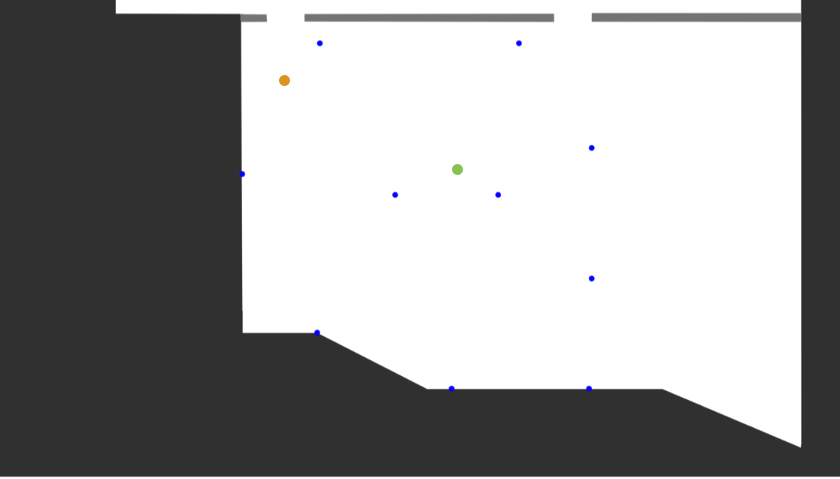
\includegraphics[width=0.45\textwidth]{figures/eval_2_10B}
	}
	\subfloat[8 Beacons] {
		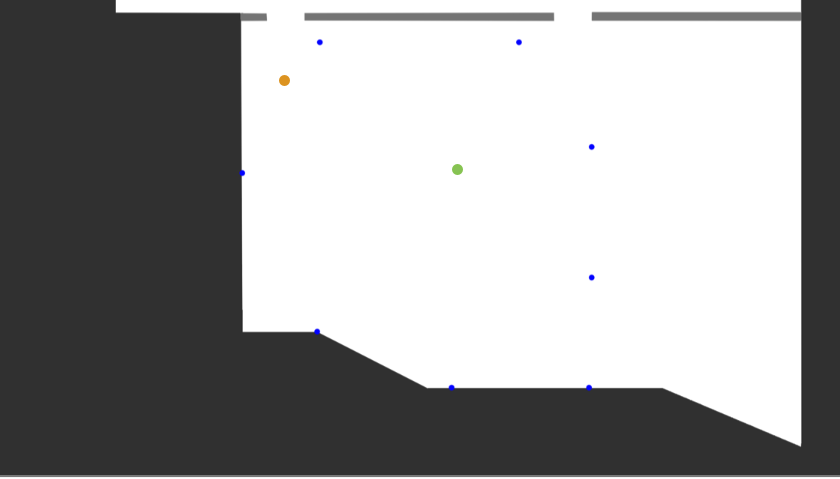
\includegraphics[width=0.45\textwidth]{figures/eval_2_8B}
	}
	
	\subfloat[6 Beacons] {
		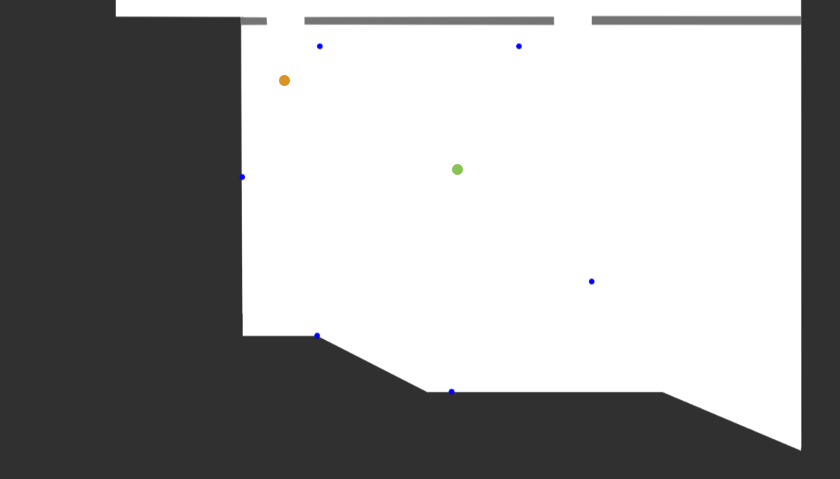
\includegraphics[width=0.45\textwidth]{figures/eval_2_6B}
	}
	\subfloat[4 Beacons] {
		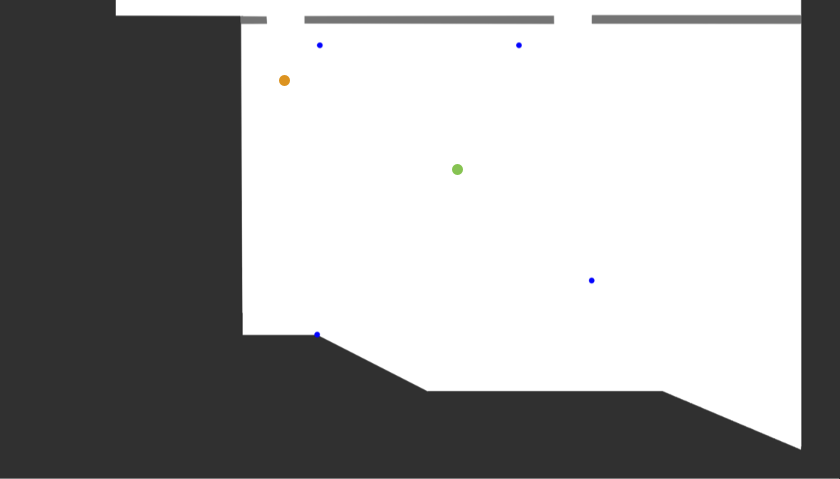
\includegraphics[width=0.45\textwidth]{figures/eval_2_4B}
	}
	
	\subfloat[2 Beacons] {
		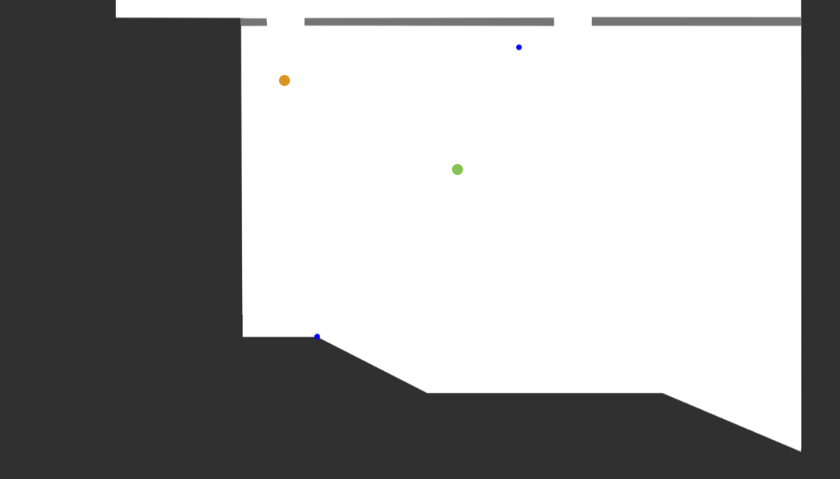
\includegraphics[width=0.45\textwidth]{figures/eval_2_2B}
	}

	\caption{Shows the different beacon deployments during the experiment.}
	\label{fig:exp2_imgs}
\end{figure}


\subsection*{Experiment~3}
After evaluating the solution's accuracy in the first two experiments, this experiment shows how good the solution is able to track an users path in a larger scenario. Therefor, we additionally used the buildings foyer, depicted in figure~\ref{fig:f-foyer}, and one, resp.\ two additional lecture halls. During the examples, we still used just 10 beacons, as shown on the maps, which depict an actual space of $22.22~m \times 33.06~m$.

The first example is depicted in figure~\ref{fig:exp2_imgs}. The green line illustrates approximately the actual path, beginning at the top right. The black dashed line shows the motion path; which is just the combination of pedometer and heading. The estimated path is marked as blue dashed path. Figure~\ref{fig:exp2_imgs_1} shows, an example where the motion was very accurate, actually more accurate than the actual estimated path; whereas, figure~\ref{fig:exp2_imgs_2}, \ref{fig:exp2_imgs_3}, and~\ref{fig:exp2_imgs_4} depict examples, where the motion path is bad, resp.\ completely wrong, but the algorithm was more or less able to approximate the actual path.

Figure~\ref{fig:exp2_imgs_5} depicts another example, where the test person walked around the big stair in the middle of the buildings foyer. The screenshot shows, that the algorithm also was able to approximate this path. During this example the foyer was equipped with just 4 beacons, as shown on the map. But, we found out, that 4 beacons are to less for such a large area, if the motion is incorrectly.

Another example path is shown in figure~\ref{fig:exp2_imgs_6}. During this example the wall between the two upper halls was opened. As we can see, the algorithm was able to track the path, but fairly we have to say, that this would also not be possible without having such an accurate motion, by using just 10 beacons. The screenshot also shows, that the estimated end pose is actually not at the true position, but rather $\approx 4-5~m$ too distant. But it also shows, that two particles are located next to the right position, and that the plotted $\sigma-\text{ellipse}$ is oriented towards these two particles.  The reason therefor is, that the algorithms weight sum dropped below the threshold, and thus, recovery was executed. Unfortunately, we stopped the recording at this point in time, otherwise its very likely that the particle cloud would jump to the true location, where the two particles are already being located. 


\begin{figure}
	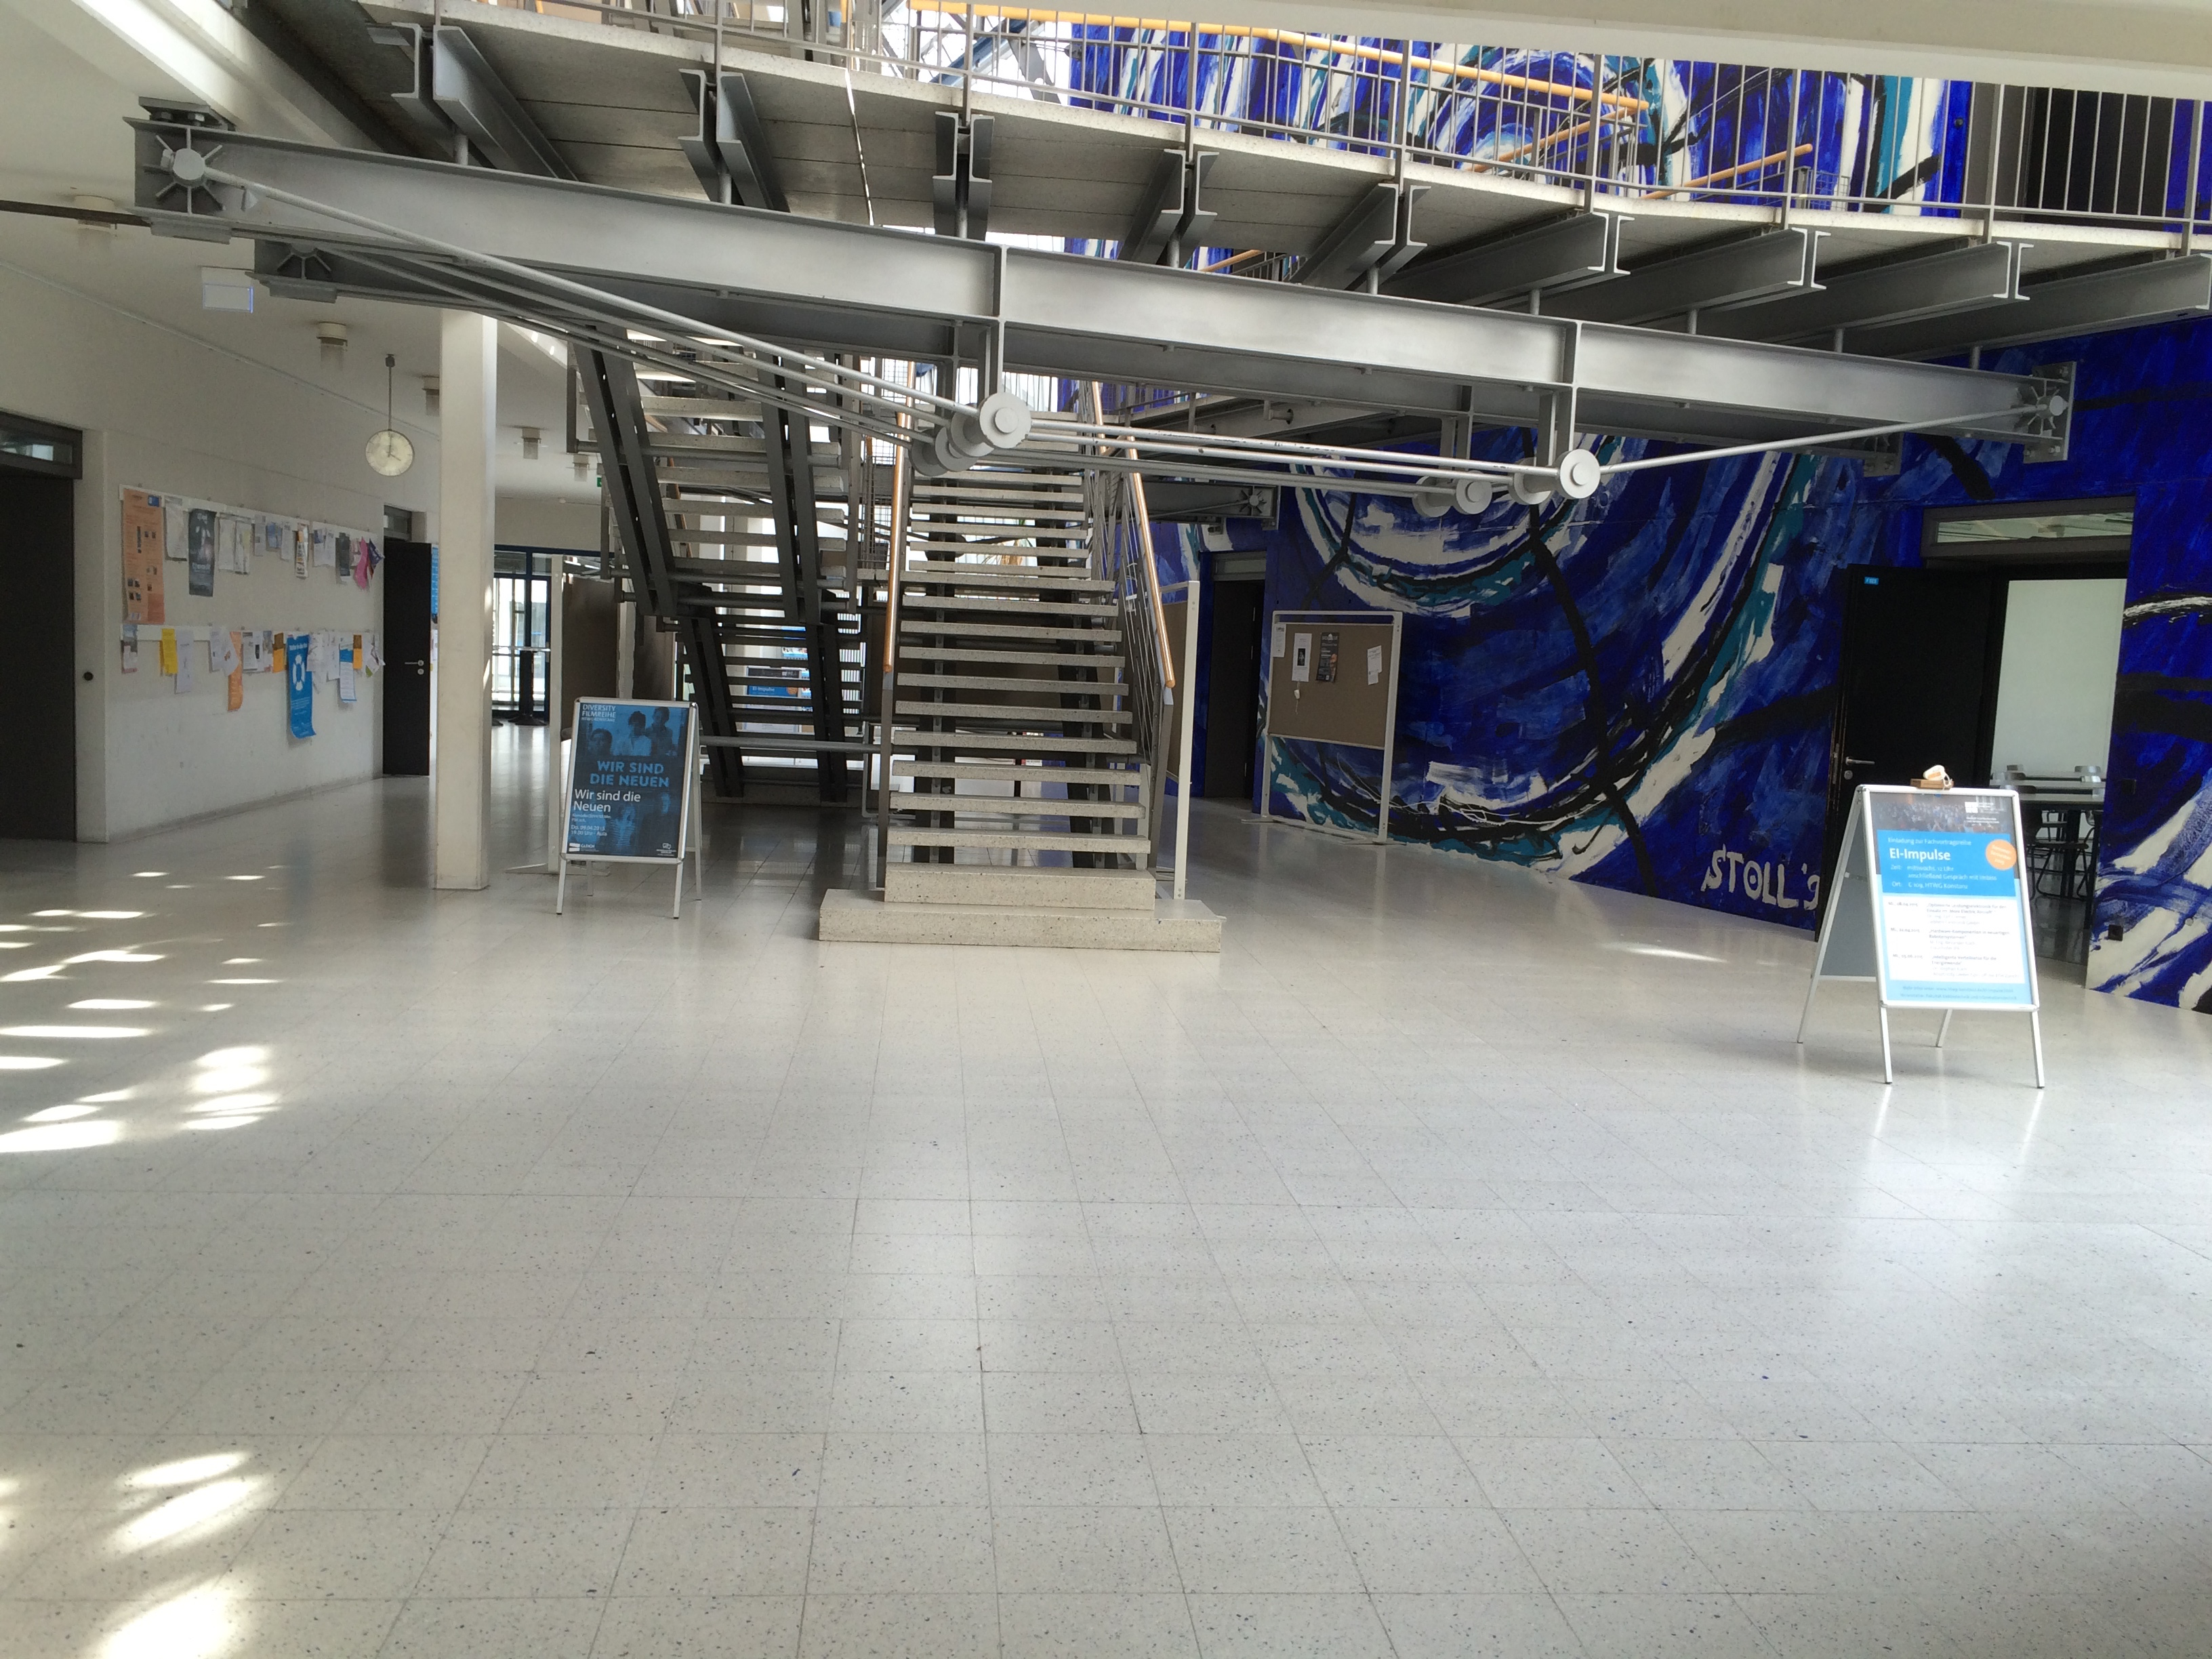
\includegraphics[width=0.9\textwidth]{figures/F-Foyer}
	\caption{Shows the buildings Foyer depicted on the map's middle.}
	\label{fig:f-foyer}
\end{figure}

\begin{figure}
	\subfloat[] {
		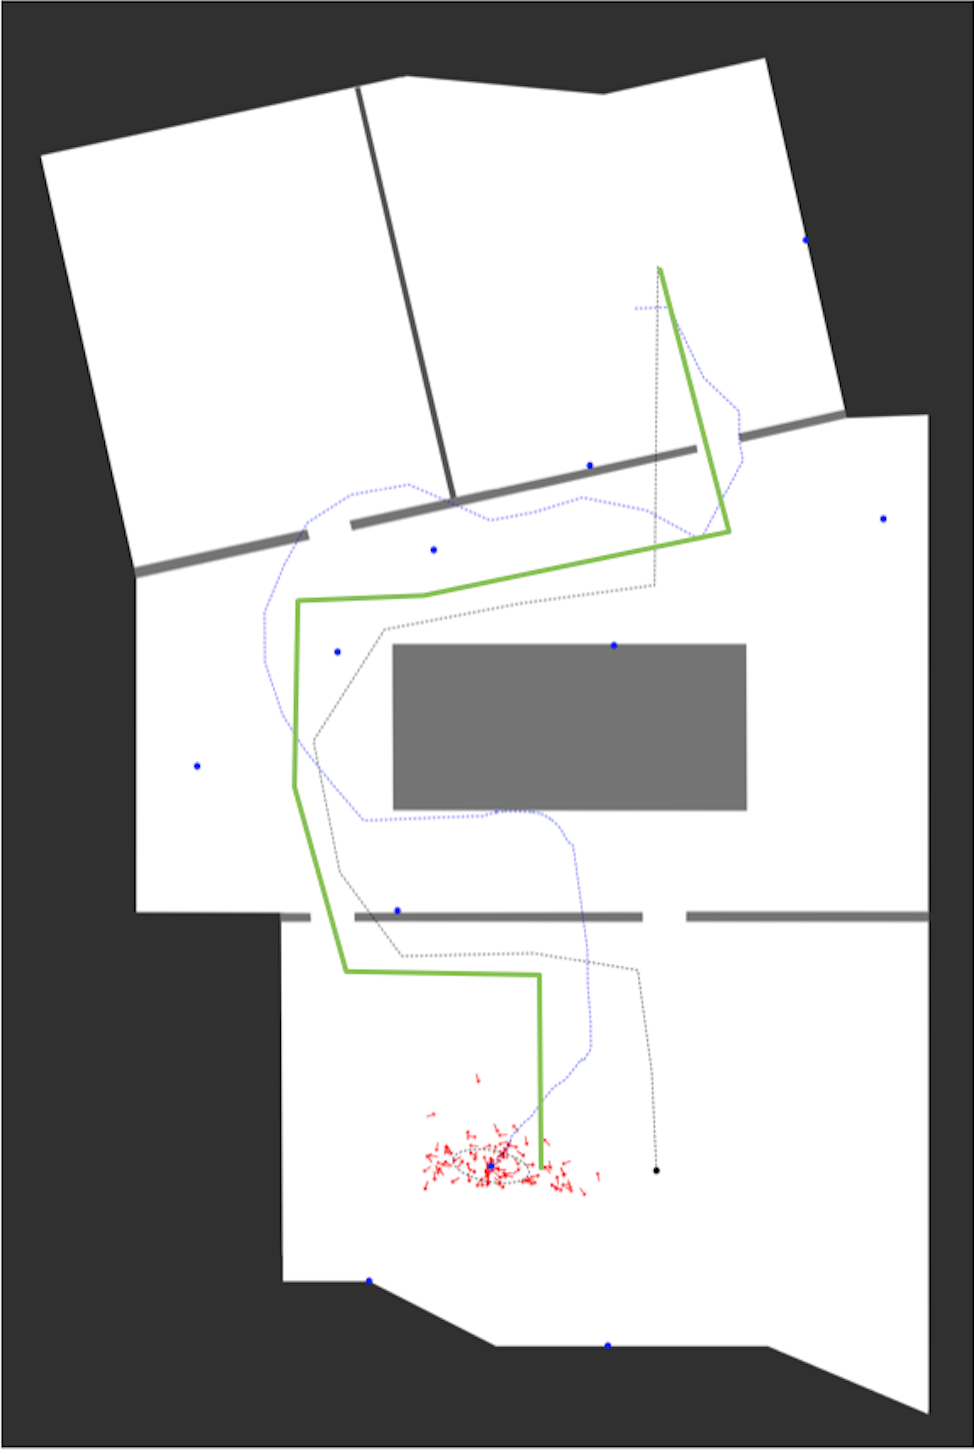
\includegraphics[height=0.45\textheight]{figures/eval_3_1}
		\label{fig:exp2_imgs_1}
	}
	\subfloat[] {
		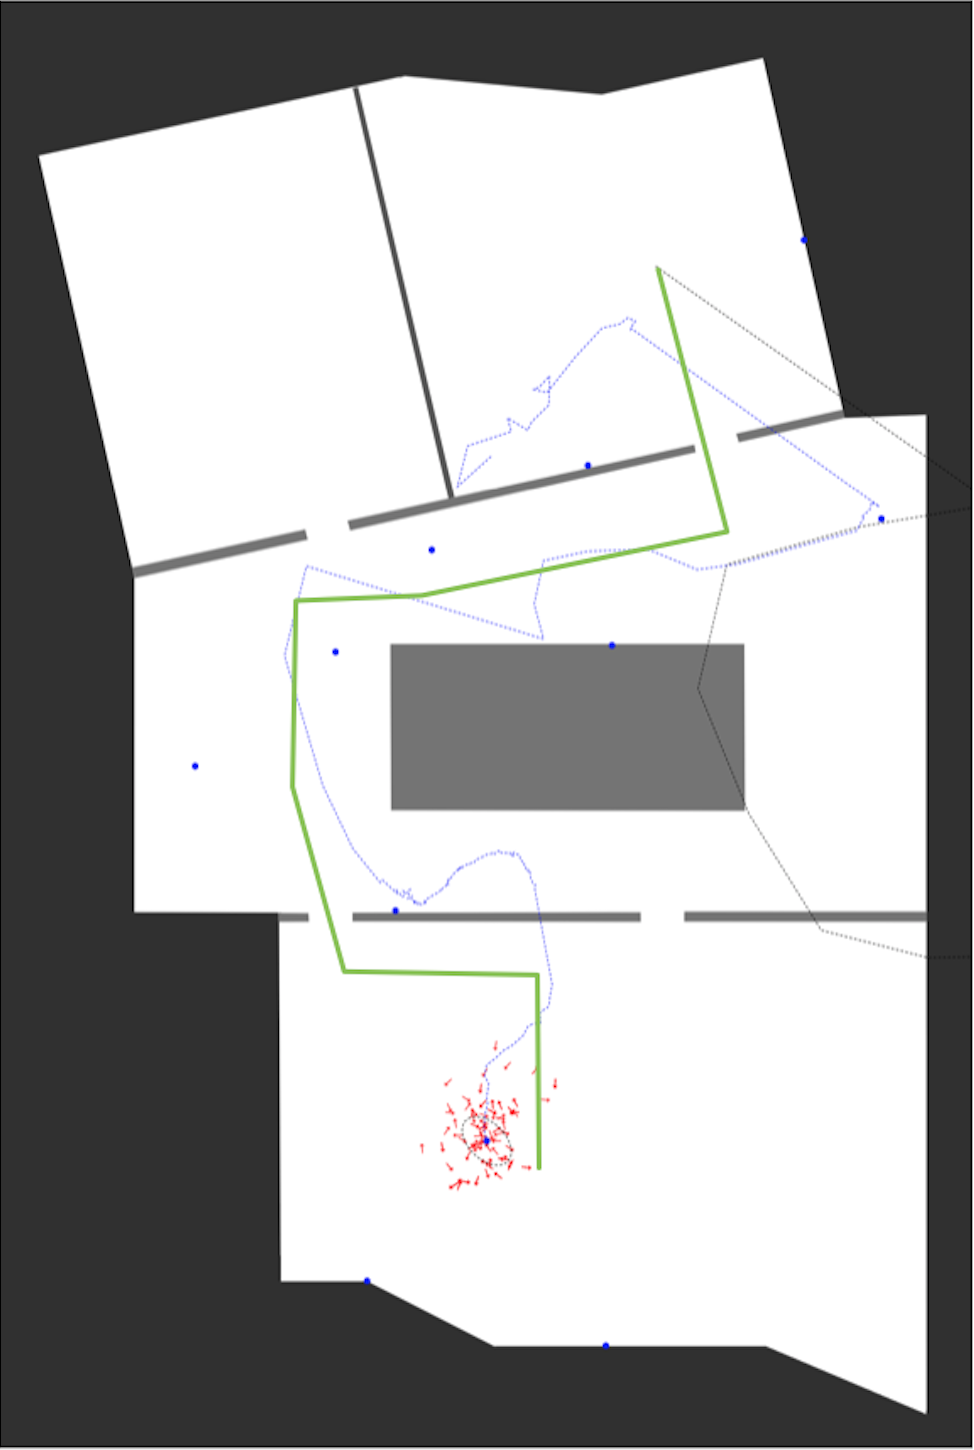
\includegraphics[height=0.45\textheight]{figures/eval_3_2}
		\label{fig:exp2_imgs_2}
	}
	
	\subfloat[] {
		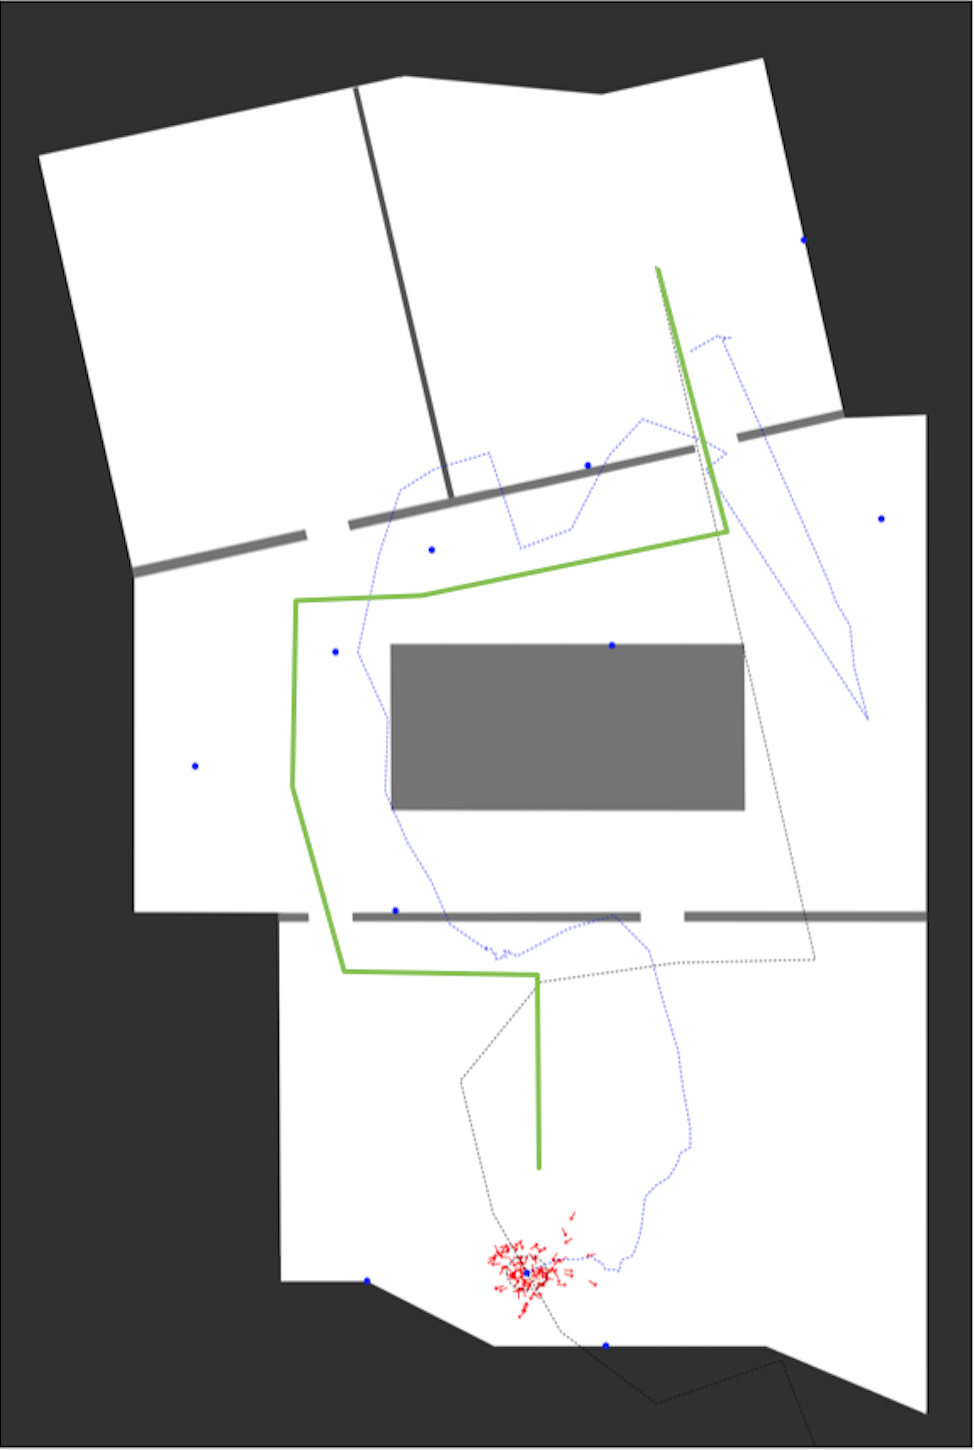
\includegraphics[height=0.45\textheight]{figures/eval_3_3}
		\label{fig:exp2_imgs_3}
	}
	\subfloat[] {
		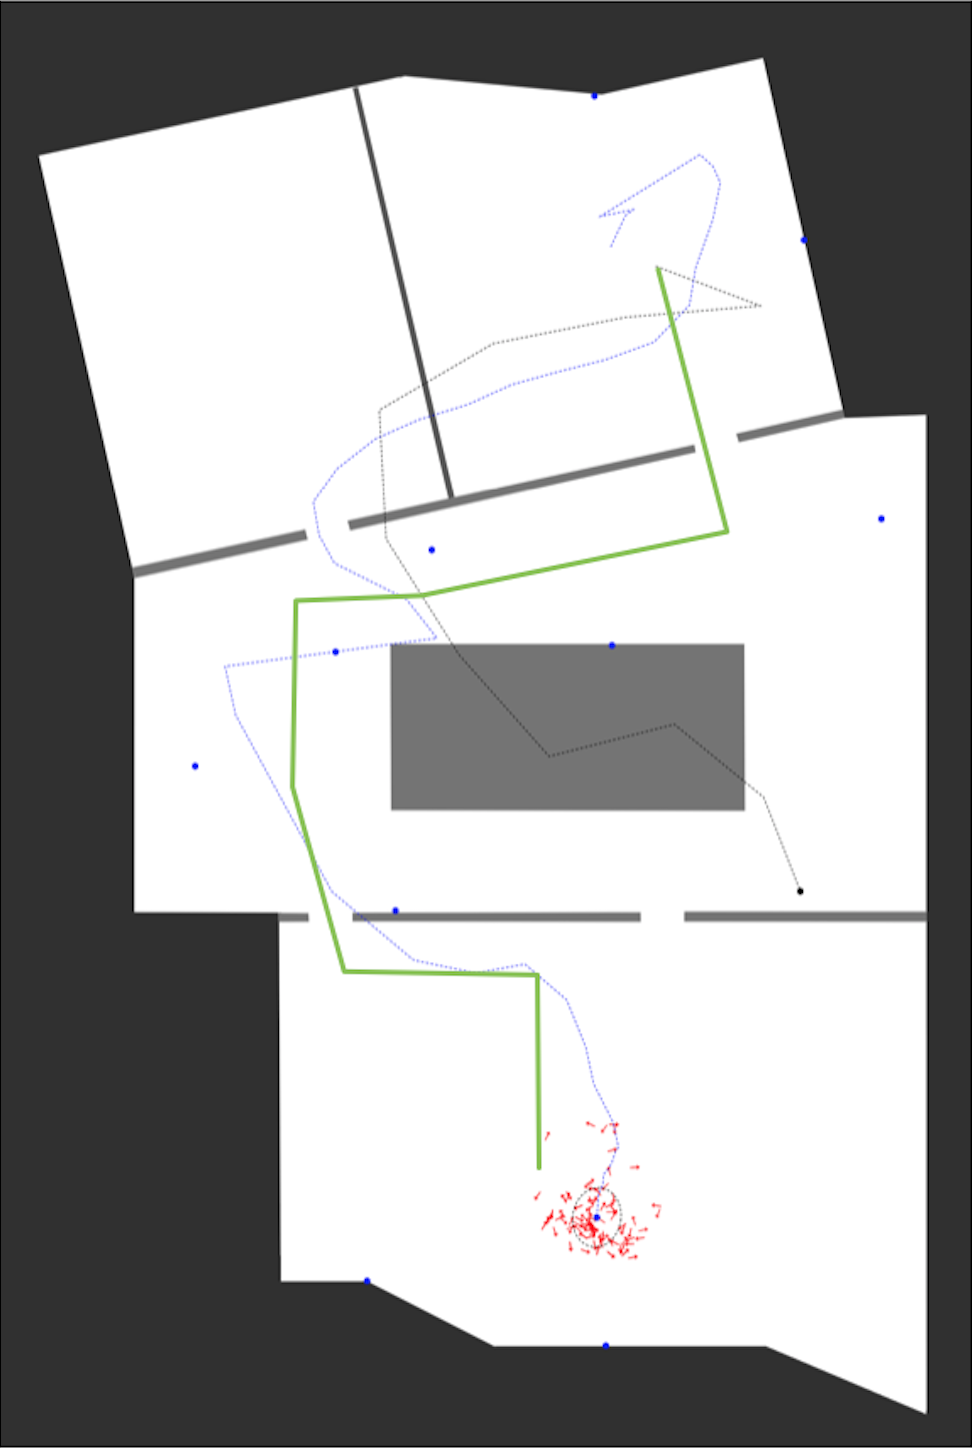
\includegraphics[height=0.45\textheight]{figures/eval_3_4}
		\label{fig:exp2_imgs_4}
	}
	\caption{Shows the different beacon deployments during the experiment.}
	\label{fig:exp2_imgs}
\end{figure}

\begin{figure}
	\subfloat[] {
		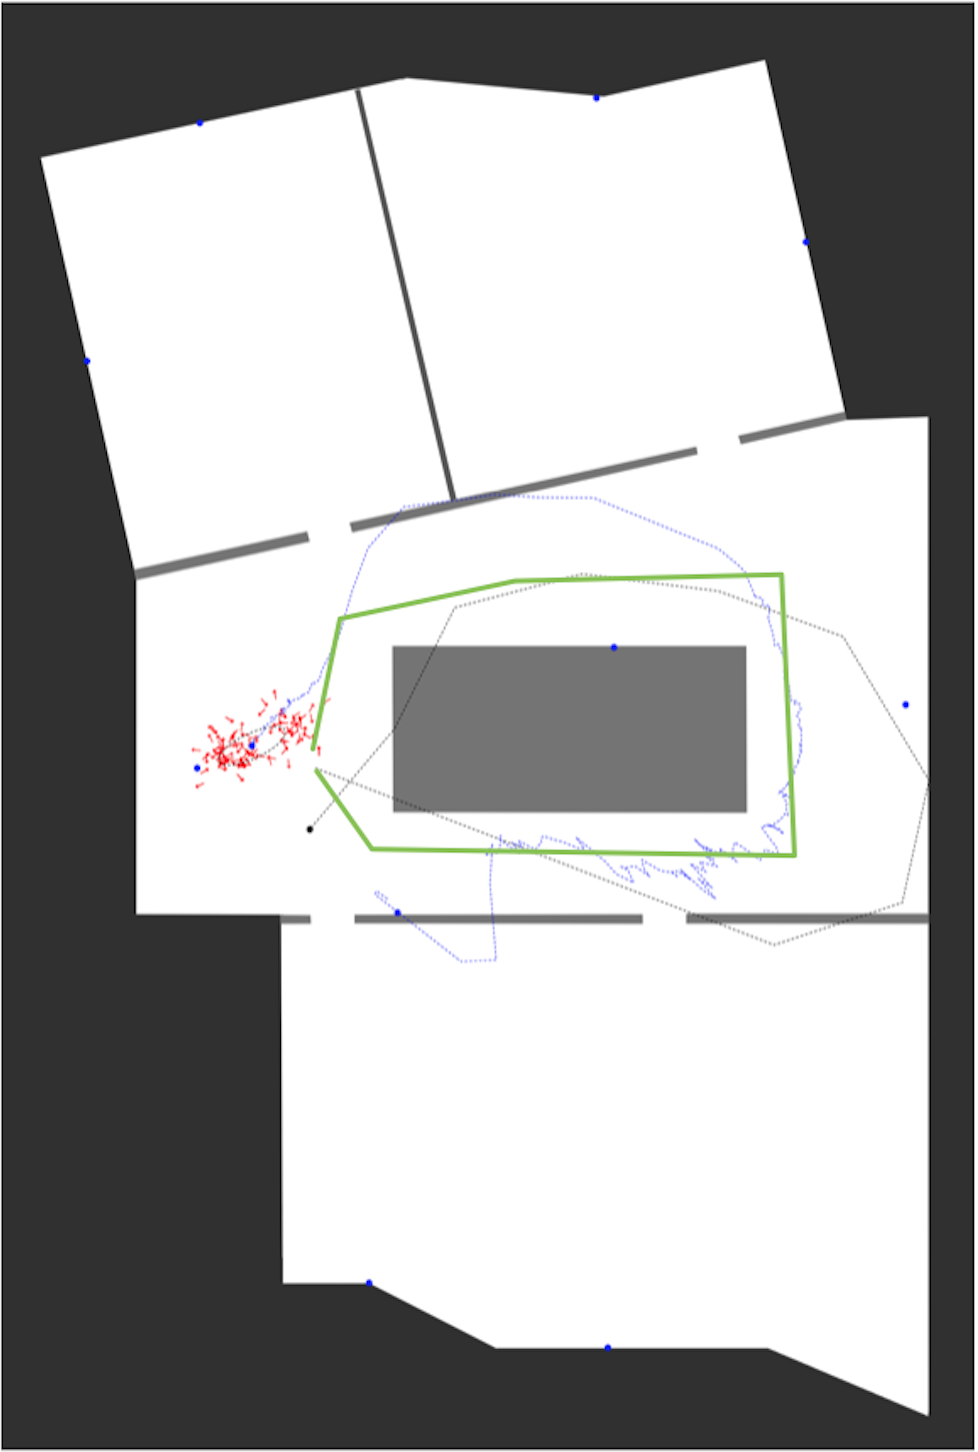
\includegraphics[height=0.45\textheight]{figures/eval_3_5}
		\label{fig:exp2_imgs_5}
	}
	\subfloat[] {
		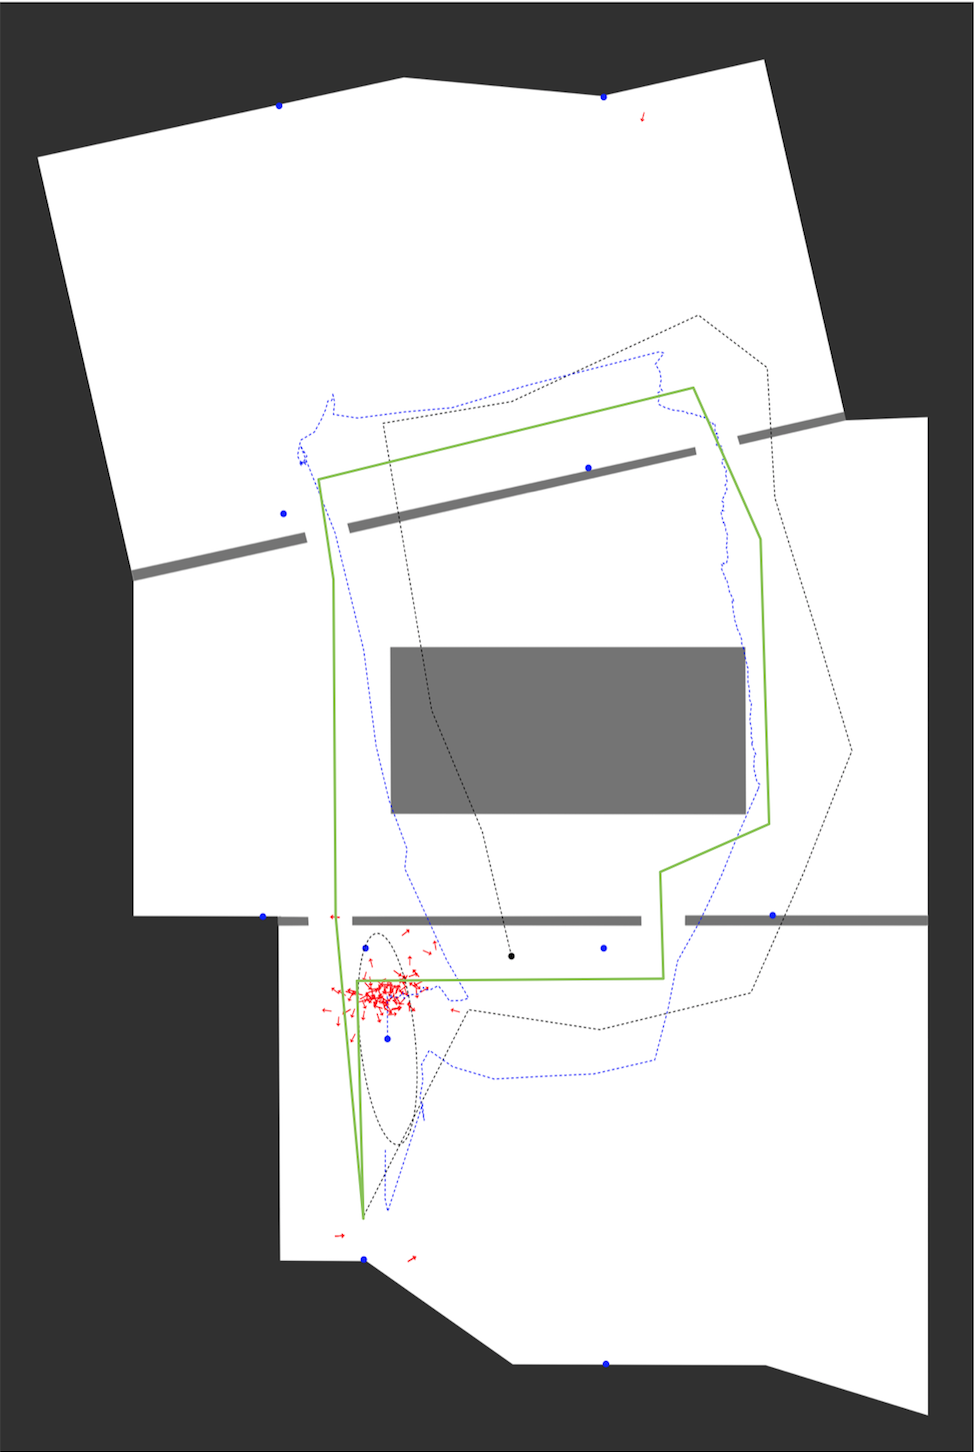
\includegraphics[height=0.45\textheight]{figures/eval_3_6}
		\label{fig:exp2_imgs_6}
	}
	\caption{Shows the different beacon deployments during the experiment.}
\end{figure}


\subsection*{Summary}
We tested our algorithm in a typical environment, with enabled WiFi, obstacles and lots of reflecting material, as shown on the building's images.

The experiments approve, that the estimation's accuracy depends on the amount of deployed beacons, but also on their position and attitude relative to the user, which influences the beacons's signals. Furthermore, we found out, that the estimated position not just depends on the beacons's signal's, it also depends on the motion's quality. As shown by experiment~3, location estimation is possible with having too less beacons deployed, but therefor the motion must be relatively correct. But, it also shows, that if enough beacons are deployed, our solution is able to correct the path, on the basis of the beacon's signals.

We also found out, that the location estimation improves after being stationary for a few seconds, if enough beacons are deployed.

Due to the fact that the application's accuracy and precision depends on so many different factors, we can just point out, what the system reached during our experiments, but we cannot provide, in general valid precision and accuracy values for the system. During our experiments we reached an accuracy up to 1.52~meters (experiment 2). By combining the results of experiment 1 and 2 (with 10 beacons), our application reached an accuracy of 2.12~meters ($\mu=2.12$, $\sigma=2.72$). Our applications precision, expressed as commutative distribution function (CDF), is shown in figure~\ref{fig:eval:precision}.

To summarize, our solution provides at least room level accuracy, even better accuracy, depending on the deployed beacon count and other parameters. Furthermore, our solution is able to track a user's path, in environments with lots of free space, as shown by the experiments; thus, its ability to track a user in corridors should also be very good, due to the fact that we take the map's free space into account. The solutions only disadvantage is, that the user has to hold the device in hand pointing into the user's walking direction, otherwise the motion's orientation is completely wrong, and thus, recovery often needs to be executed.

\pgfmathdeclarefunction{cdf}{2}{%
  \pgfmathparse{1/(1 + exp(-0.07056*((x-#1)/#2)^3 - 1.5976*(x-#1)/#2))}%
}


\begin{figure}
	\begin{tikzpicture}
	\begin{axis}[trim axis left, trim axis right, height=0.4\textheight,
		xlabel={Error / Accuracy $x$ (m)},
		ylabel={$CDF(x)$},
		legend entries={Exp.\ 1, Exp.\ 2, Exp.\ 1+2},
		legend pos=south east,
		grid = major]
		\addplot[red, smooth, mark=no, domain=-6.08:10.66] {cdf(2.29, 2.97)};
		\addplot[blue, smooth, mark=no, domain=-6.08:10.66] {cdf(1.52, 1.79)};
		\addplot[green, smooth, mark=no, domain=-6.08:10.66] {cdf(2.12, 2.72)};
	\end{axis}
\end{tikzpicture}
\caption{Depicts our solutions precision during the experiments.}
\label{fig:eval:precision}
\end{figure}


% depends on the beacons position
% on the location in the room
% on the building
% on the beacons itself
% -> on beacons signals, and motion quality

\section{Scalability}
The area covered from our localization system, depends just on the provided map and deployed beacons. Thus, our system is highly scalable. It can just be used within a single room, but it also can be extended, to a very large, two-dimensional space.

\section{Robustness}
The system is very robust. It can deal with wrong and / or missing beacon signals, which is a very common problem. Furthermore, it is able to deal with wrong motion data, caused by influenced heading or wrong distance estimations provided by the pedometer, as shown by the experiments.

Due to the implemented recovery from failure state, it is also able to detect completely wrong position estimations; for instance, caused by the kidnapping problem. The only requirement for the recovery is, that the application needs to at least receive the signal of one beacon.

\section{Complexity}
The solutions complexity is relatively low. Besides the beacons, and a common smartphone, no additional infrastructure such as, a network connection or external power supply, is required.
	
Also, the software complexity is relatively low, due to the used particle filter algorithm. Of course, if a platform does not provide such high level \acs{API}'s, especially such as \acl{CM}'s pedometer, to estimate the walked distance, this low level of complexity would not be possible.

\section{Cost}
The system's biggest advantages regarding costs are, that besides the beacons no additional infrastructure is required, and the users can use their own smartphones.

Consequently, the system's cost mainly depends on the to be covered area, and thus, on the required amount of beacons, and the initial deployment and setup costs. 100 beacons (incl.\ batteries) from BEACONinside do cost 1790~EUR, but there are also cheaper manufacturers.

Furthermore, the system's maintenance effort is relatively low. Typically, the beacons's batterie's lifetime is up to a year or more. And, as long as no big changes are made to the beacon's environment, recalibration is not necessary.

\section{Usability}
The localization system is very easy to use. The user just has to download the App from the platform's app store. After enabling and giving the application access to \acl{BT}, the localization can start.

The user interface can also be reduced to a minimum, by just showing the environments map, the estimated position and the corresponding $\sigma-\text{ellipse}$, instead of showing the beacons, the motion path, the user's estimated path, and the particle cloud.

There is just one disadvantage from an usability point of view, which is the position estimation's delay. If the user walks, the estimated position is just being updated ever $\approx 3~\text{sec}$, due to the fact, that \acs{CM} just provides a distance estimation every $\approx 2.5~\text{sec}$, as mentioned in chapter~\ref{chap:pf}. If the user is stationary, the delay drops to $\approx 1~\text{sec}$, which is from our point of view, negligible. 

\chapter{Conclusion} \label{chap:conclusion}
% starke verzögerung (2.5 sec - 3sec)
% also usability während dem drauf schauen lackt
% stark von der qualität der odometrie und signalen abhänig
\section{Future Work} \label{sec:future}

\begin{itemize}
	\item Beacons an die Decke hängen
	\item Noch mehr Beacons verteilen
	\item Beacons anderer Hersteller testen
	\item Barometer von iPhone 6 + Neuer Motion Chip M8
	\item nicht nur 2D sondern auch 3D
	\item Multi-Robot localization problem. Smartphone could appear as an additional beacon or tell new devices that are very close to it its localized position
	\item Define beacon regions to adjust parameters of filter to be more accurate (zwischen Einkaufsregalen)
\end{itemize}


%\appendix
%\chapter{Build-in Sensor Evaluation}
% CMPedometer (step count, distance) error plots
\begin{figure}[htbp]
  \subfloat[Distance error]{
    \begin{tikzpicture}
      \begin{axis}[width=0.45\textwidth, height=0.4\textheight,
          xlabel={Reference distance (m)},
          ylabel={Average distance error (m)},
          legend entries={in hand, in pants pocket},
          legend pos=north west,
        grid = major]
        \addplot [blue, only marks, mark=*] table[col sep=semicolon, x=distanceRef, y=distanceError] {csv/2014-10-28_htwg_keller_f/inHand_avg.csv};
        \addplot [red, only marks, mark=*] table[col sep=semicolon, x=distanceRef, y=distanceError] {csv/2014-10-28_htwg_keller_f/inPocket_avg.csv};
      \end{axis}
    \end{tikzpicture}
  }
  \quad
  \subfloat[Step count error]{
    \begin{tikzpicture}
      \begin{axis}[width=0.45\textwidth, height=0.4\textheight,
          xlabel={Reference distance (m)},
          ylabel={Average step count error},
          legend entries={in hand, in pants pocket},
          legend pos=north west,
        grid = major]
        \addplot [blue, only marks, mark=*] table[col sep=semicolon, x=distanceRef, y=stepError] {csv/2014-10-28_htwg_keller_f/inHand_avg.csv};
        \addplot [red, only marks, mark=*] table[col sep=semicolon, x=distanceRef, y=stepError] {csv/2014-10-28_htwg_keller_f/inPocket_avg.csv};
      \end{axis}
    \end{tikzpicture}
  }
  \caption{Measurement curicumstances: The measurements where taken indoor (HTWG Konstanz cellar F building).}
\end{figure}


\addcontentsline{toc}{chapter}{References}
%\bibliographystyle{IEEEtranS}
\bibliographystyle{apa}
%\nocite{*}
\bibliography{chapters/99_references}

\end{document}
